\documentclass[12pt, a4paper]{report}
\usepackage[utf8]{inputenc}
\usepackage{graphicx}
\usepackage{natbib}
\usepackage{amsmath}
\usepackage{multirow}
\usepackage{hyperref}
\usepackage[left=1in, right=1in, top=1in, bottom=1in]{geometry}

\setkeys{Gin}{draft=True} %if True, all figures will print as just an empty box (useful when you don't want to wait for an entire dissertation with figures to compile)

% define sympols
\newcommand{\degree}{$\,^o\,$}
\newcommand{\almost}{$\,\sim\,$}
\newcommand{\rsun}{$\,R_\odot\,$}
\newcommand{\percc}{$\,cm^{-3}\,$}
\newcommand{\kms}{$\,km\,s^{-1}\,$}

% Custom commands or styles can go here
%\includeonly{chapter1/ch1} % Include only Chapter 1




\begin{document}

\begin{titlepage}
    \begin{center}
        \vspace*{1cm}
        
        \Huge
        \textbf{From the Sun to Earth: Exploring the Multifaceds of Solar Eruptive Events}
        
        \vspace{1.5cm}
        
        \LARGE
        Mohamed Nedal
        
        \vfill
        
        A thesis submitted for the degree of\\
        Doctor of Philosophy
        
        \vspace{0.8cm}
        
        \Large
        Institute of Astronomy and National Astronomical Observatory, Bulgarian Academy of Sciences\\
        Solar and Space Weather Research\\
        \today
        
        \vspace{0.8cm}
        
        Supervisor: Assoc. Prof. Kamen Asenov Kozarev
        
    \end{center}
\end{titlepage}


\pagenumbering{roman}

\chapter*{Abstract}
The following are the 3 abstracts of my 3 main papers. Merge them together in a single abstract with a narrative story ...

We present a comprehensive characterization of 61 Coronal Mass Ejection (CME)-driven compressive waves known as Coronal Bright Fronts (CBFs) observed in the low solar corona between 2010 and 2017. These CBFs have been found to be associated with Solar Energetic Particle (SEP) events near Earth, indicating their importance in understanding space weather phenomena.
The aim of this study is to analyze and describe the early dynamics of CBFs using a physics-based heliospheric SEP forecasting system known as the Solar Particle Radiation Environment Analysis and Forecasting - Acceleration and Scattering Transport (SPREAdFAST) framework. This framework utilizes a chain of data-driven analytic and numerical models to predict SEP fluxes at multiple locations in the inner heliosphere by considering their acceleration at CMEs near the Sun and subsequent interplanetary transport.
To estimate the time-dependent plasma and compression parameters of the CBFs, we utilized sequences of base-difference images obtained from the Atmospheric Imaging Assembly (AIA) instrument on board the Solar Dynamics Observatory (SDO) satellite, and measurements of the height-time profiles of the coronal waves obtained from the Large Angle and Spectrometric COronagraph (LASCO) instrument on board the Solar and Heliospheric Observatory (SOHO) satellite. We employed kinematic measurements and plasma model results to derive these parameters. The SPREAdFAST framework facilitated the analysis and correlation of these observations with SEP events near Earth.
Our analysis yielded statistical relations and distributions for both the shocks and plasma parameters associated with the 61 CBFs investigated. By combining the observations from the AIA and LASCO instruments, as well as the data products from the SPREAdFAST framework, we obtained a comprehensive understanding of the early dynamics of CBFs, including their temporal evolution, plasma properties, and compressional characteristics. These findings contribute to the growing body of knowledge in the field and have implications for space weather forecasting and the study of SEP events.

This study aims to investigate the ambiguous source and the underlying physical processes of the type III radio bursts that occurred on April 3, 2019, through the utilization of multi-wavelength observations from the Low-Frequency Array (LOFAR) radio telescope and the Parker Solar Probe (PSP) space mission, as well as incorporating results from a Potential Field Source Surface (PFSS) and magnetohydrodynamic (MHD) models. The primary goal is to identify the spatial and temporal characteristics of the radio sources, as well as the plasma conditions along their trajectories.
We applied data preprocessing techniques to combine high- and low-frequency observations from LOFAR and PSP between 2.6 kHz and 80 MHz. We then extracted information on the frequency drift and speed of the accelerated electron beams from the dynamic spectra. Additionally, we used LOFAR interferometric observations to image the sources of the radio emission at multiple frequencies and determine their locations and kinematics in the corona. Lastly, we analyzed the plasma parameters and magnetic field along the trajectories of the radio sources using PFSS and MHD model results.
We present several notable findings related to type III radio bursts. Firstly, through our automated implementation, we were able to effectively identify and characterize 9 type III radio bursts in the LOFAR-PSP combined dynamic spectrum and 16 type III bursts in the LOFAR dynamic spectrum. We found that the frequency drift for the detected type III bursts in the combined spectrum ranges between 0.24 and 4 MHz s$^{-1}$, while the speeds of the electron beams range between 0.013 and 0.12 C. Secondly, our imaging observations show that the electrons responsible for these bursts originate from the same source and within a short time frame of fewer than 30 minutes. Finally, our analysis provides informative insights into the physical conditions along the path of the electron beams. For instance, we found that the plasma density obtained from the magnetohydrodynamic algorithm outside a sphere (MAS) model is significantly lower than the expected theoretical density.
   
Solar energetic particles are mainly protons and originate from the Sun during solar flares or coronal shock waves. Forecasting the Solar Energetic Protons (SEP) flux is critical for several operational sectors, such as communication and navigation systems, space exploration missions, and aviation flights, as the hazardous radiation may endanger astronauts’, aviation crew and passengers’ health, the delicate electronic components of satellites, space stations, and ground power stations. Therefore, the prediction of the SEP flux is of high importance to our lives and may help mitigate the negative impacts of one of the serious space weather transient phenomena on the near-Earth space environment. Numerous SEP prediction models are being developed with a variety of approaches, such as empirical models, probabilistic models, physics-based models, and AI-based models. In this work, we use the bi-directional long short-term memory (BiLSTM) neural network model architecture to train SEP forecasting models for 3 standard integral GOES channels ($>$10 MeV, $>$30 MeV, $>$60 MeV) with 3 forecast windows (1-day, 2-day, and 3-day ahead) based on daily data obtained from the OMNIWeb database from 1976 to 2019. As the SEP variability is modulated by the solar cycle, we select input parameters that capture the short-term, typically within a span of a few hours, and long-term, typically spanning several days, fluctuations in solar activity. We take the F10.7 index, the sunspot number, the time series of logarithm of the x-ray flux, the solar wind speed, and the average strength of the interplanetary magnetic field as input parameters to our model. The results are validated with an out-of-sample testing set and benchmarked with other types of models.


\chapter*{Acknowledgments}
For my family ...

\tableofcontents
\listoftables
\listoffigures
%\newpage

\pagenumbering{arabic}

\chapter{Introduction}
\label{chapter1}

\section{Background and Motivation}
The Sun, an ordinary main-sequence star situated at the center of our Solar System, exhibits various forms of activity and variability on multiple spatial and temporal scales One of the main manifestations of solar activity relevant to space weather research are transient energetic eruptive phenomena such as flares, Coronal Mass Ejections (CME), and wide-ranging emissions of electromagnetic radiation and energetic particles \citep{schwenn_2006, pulkkinen_2007}. These eruptive events originate due to the sudden release of free magnetic energy stored in complex, twisted or sheared magnetic field structures in the solar atmosphere \citep{moore_2001, priest_forbes_2007, zhang_2012, amari_2014}. The energetic phenomena are driven by the rapid dissipation of magnetic energy via magnetic reconnection which can accelerate large numbers of electrons to relativistic energies and heat plasma to tens of million Kelvin \citep{shibata_2011, benz_2017}.

The eruptive solar events drive major disturbances in the near-Earth space environment and planetary environments across the heliosphere, collectively termed space weather \citep{schrijver_2010, eastwood_2017}. Enhanced fluxes of solar energetic particles (SEPs), plasma ejecta, and electromagnetic radiation emitted during solar eruptions can impact the geomagnetic field, radiation belts, ionosphere, thermosphere, and upper atmosphere surrounding the Earth \citep{schwenn_2006, pulkkinen_2007}. Adverse effects range from disruption of radio communications to damage of satellites, power grid failures, aviation hazards due to radiation risks for airline crew and passengers, and increased radiation exposure for astronauts \citep{lanzerotti_2001}. The societal dependence on space-based infrastructure has increased exponentially, escalating the vulnerability to space weather disturbances. Recent studies estimate a severe space weather event could lead to trillion-dollar economic damages in the US alone \citep{oughton_2017}. Besides the near-Earth space environment, solar eruptive transients also drive adverse space weather effects across the Solar System impacting activities such as deep space exploration and astronomy \citep{lilensten_2014}.

Therefore, advancing our understanding of the origins and propagation characteristics of solar eruptive phenomena, as well as quantifying their impacts on geospace and planetary environments, has become an extremely important pursuit for nations worldwide Fundamental research seeks to uncover the physical processes involved using observations coupled with theory and modeling. Concurrently, significant efforts are underway to develop next-generation space environment modeling and forecasting capabilities for predicting the impacts of solar variability. The field combining these research and predictive aspects related to Sun-Earth connections is broadly termed heliophysics \citep{schrijver_siscoe_2010}. It encompasses understanding the fundamental solar, heliospheric and geospace plasma processes; coupling across multiple spatial and temporal scales; quantifying the impacts on humanity's technological systems and space-borne assets; and utilizing this knowledge to prevent/mitigate adverse effects \citep{schrijver_2015a, schrijver_2015b}. NASA's Living With a Star program and the National Science Foundation's Space Weather activities exemplify strategic efforts to advance scientific understanding and predictive capabilities across the interconnected domains of heliophysics \citep{brewer_2002}.

The present thesis focuses on studying several important phenomena related to solar eruptive activity and its impacts from the perspective of heliophysics research and space weather. The specific topics investigated include: (1) The propagation and evolution characteristics of large-scale coronal disturbances termed EUV waves that are triggered by solar flares and CMEs; (2) The generation, propagation and plasma characteristics of solar radio bursts emitted by accelerated electron beams traveling along open magnetic field lines in the corona; (3) The forecasting of gradual solar energetic particle (SEP) events which constitute one of the major components of space radiation hazards at Earth.

These diverse topics are united by the common theme of seeking to uncover the origins and propagation mechanisms of key transient phenomena resulting from solar eruptions, utilizing observational data, analytical theory and modeling, and data science techniques. The phenomena have been studied for several decades using observations from multiple space missions, but gaps persist in our understanding of their underlying physics and space weather impacts. The thesis aims to provide new insights that help address some of the outstanding questions, guided by the overarching goals and framework of heliophysics research. The following sub-sections elaborate on the background, significance, observational challenges and knowledge gaps pertaining to each of the research topics investigated. The following subsection provide a concise overview of key literature related to the research topics investigated in the thesis. A detailed review is presented in each chapter specific to the respective phenomenon.

\subsection{Coronal Waves}
Coronal waves, or Coronal Bright Fronts (CBFs), also known as Extreme Ultra-Violet (EUV) waves, are large-scale arc-shaped bright fronts or disturbances observed propagating across significant portions of the solar corona following the eruption of CMEs and flares \citep{thompson_1998, nindos_2008, vrsnak_2008, magdalenic_2010, veronig_2010, warmuth_2015}. They are best observed in EUV and white-light coronal emission, as well as in radio wavelengths, spanning distances of up to several 100 Mm with speeds ranging from 100-1000 \kms, faster than the local characteristic speed in the solar corona, transforming into shock waves \citep{liu_2014, pick_2006, thompson_2009, nitta_2013}. These structures consist of piled-up plasma with higher density, making them appear brighter in white-light images.

The discovery of coronal waves dates back to observations obtained with the EIT instrument on SOHO launched in 1995, appearing as bright propagating fronts in 19.5 nm wavelength imaging of Fe XII emission lines formed at \almost1.5 MK plasma \citep{thompson_1998}. Subsequent studies based on SOHO/EIT and TRACE imaging found correlations between waves and CMEs, favoring an interpretation as fast-mode MHD waves driven by CME lateral expansions \citep{biesecker_2002}.

Since 2010, the initiation and evolution of coronal waves are being exquisitely observed with unprecedented resolution by the Atmospheric Imaging Assembly (AIA) on the Solar Dynamics Observatory (SDO) instrument \citep{lemen_2012} across multiple EUV passbands sensitive to a wide temperature range \citep{nitta_2013}. Alternatively, shock waves can be indirectly observed through the detection of type II radio bursts, which are commonly associated with shock waves in the solar corona \cite{vrsnak_2008}.
The AIA instrument has provided valuable insights into the dynamics of the low solar corona over the past decade, thanks to its exceptional spatial and temporal resolution. Equipped with telescopes observing the solar disk in bands 193 and 211~\AA, the AIA instrument has demonstrated its ability to distinguish compressive waves in the lower corona \cite{patsourakos_2010, ma_2011, kozarev_2011}. These observations offer valuable information about the kinematics and geometric structure of CBFs. To accurately study the evolution of the wave's leading front, observations off the solar limb are preferred to mitigate projection effects, which may introduce ambiguities in estimating time-dependent positions and the global structure of the wave \cite{kozarev_2015}.

In situ observations of shock waves have revealed their classification into quasi-parallel, quasi-perpendicular, sub-critical, and super-critical shocks based on the angle between the wavefront normal vector and the upstream magnetic field lines \cite{tsurutani_1985}. Quasi-parallel shocks have an angle ($\theta_{BN}$) smaller than 45\degree, while quasi-perpendicular shocks have $\theta_{BN}$ greater than 45\degree. Supercritical shocks, often associated with accelerated particles, are promising candidates for generating type II radio bursts \cite{benz_1988}. However, obtaining accurate estimates of shock strength and obliquity solely from remote observations is challenging.

Coronal waves exhibit diverse morphology and kinematics ranging from circular fronts to narrow jets or expanding dome-like structures \citep{veronig_2010}. A taxonomy of wave properties based on extensive observational surveys can be found in papers by \citet{muhr_2014} and \citet{nitta_2013}. However, despite being observed for over two decades since their serendipitous discovery, fundamental questions remain regarding the physical nature and drivers of coronal waves \citep{chen_2016, vrsnak_2008, warmuth_2015}. The debate centers around two competing interpretations - the wave versus pseudo-wave (or non-wave) models. The wave models envisage coronal waves as fast-mode MHD waves or shocks that propagate freely after being launched by a CME lateral over-expansion or an initial flare pressure pulse \citep{wills_2007, vrsnak_2008}. The pseudo-wave models interpret them as bright fronts produced by magnetic field restructuring related to the CME lift-off process rather than a true wave disturbance \citep{delannee_1999, chen_2002}. Extensive observational and modeling studies have been undertaken to evaluate the two paradigms \citep{patsourakos_2012, long_2017}, but a consensus remains elusive. Addressing these outstanding questions related to the nature and origin of coronal waves is imperative, since they are being incorporated into models as a primary agent producing SEP events and geomagnetic storms during CMEs \citep{rouillard_2012, park_2013}. Their use as a diagnostic tool for CME and shock kinematics predictions in these models requires discriminating between the different physical mechanisms proposed for their origin.

The present thesis undertakes an extensive statistical analysis of coronal EUV wave events observed by SDO to provide new insights into their kinematical properties and relationship to CMEs. We focus on analyzing their large-scale evolution as a function of distance and direction from the source region, leveraging the extensive EUV full-disk imaging capabilities of SDO spanning nearly a decade. Statistical surveys to date have mostly focused on initial speeds and morphological classifications rather than large-scale propagation characteristics. Our study aims to uncover systematic trends in their propagation kinematics using a significantly larger sample compared to previous works. We also comprehensively evaluate associations with CME and flare parameters in order to discriminate between wave and pseudo-wave origins. The results have important implications for incorporating coronal waves into predictive models of CMEs and SEP events for future space weather forecasting.

\subsection{Solar Radio Bursts}
Solar radio emissions have been the subject of extensive study and research due to their connection with solar activity and their potential impact on Earth's atmosphere and technology. One area of particular interest is solar radio bursts, which are intense bursts of electromagnetic radiation originating from the Sun. These bursts can be classified into different types based on their characteristics and associated phenomena. Solar radio bursts, including Type III bursts, serve as remote diagnostics for the study of energetic electrons within the solar corona. These bursts result from transient energetic electron beams injected into the corona, which then propagate along interplanetary magnetic field (IMF) lines \citep{ergun_1998, pick_2006, reid_2020}. As these electron beams traverse the corona, they induce plasma waves, also known as Langmuir waves, which subsequently transform into radio emission at the local plasma frequency or its harmonic components \citep{melrose_2017}.
The frequency of the radio emission is directly linked to the plasma density, making Type III bursts a valuable tool for investigating the inner heliosphere and understanding the underlying processes that drive solar active phenomena, such as solar flares and coronal mass ejections \citep{reid_2014, kontar_2017}. These bursts offer insights into the acceleration of energetic electrons in the corona and their transport along magnetic field lines \citep{reid_2014}. The generation of electromagnetic emission at radio frequencies through plasma emission mechanisms is a key aspect of solar radio bursts, shedding light on the dynamic interplay between non-thermal electron distributions and the ambient plasma \citep{melrose_1980}.

In radio spectrograms, type III bursts manifest as intense enhancements of radio flux over background levels, exhibiting rapid frequency drifts over timescales ranging from seconds to minutes, signifying plasma dynamics \citep{reid_2017}. These bursts are observable across a wide range of frequencies, spanning from GHz to kHz, and wavelengths extending from metric to decametric \citep{wild_1950a, lecacheux_1989, bonnin_2008}. This phenomenon is detectable by ground-based instruments on Earth as well as various spacecraft within the heliosphere, underscoring the significance of plasma dynamics in their manifestation.

Pioneering observations of solar radio bursts were made in the 1940s leading to their classifications \citep{wild_1963}. Subsequent spectrographic studies uncovered emission mechanisms, source regions and particle diagnostics \citep{suzuki_1985}. Magnetic reconnection models of flares provided theoretical explanations for particle acceleration generating radio bursts \citep{holman_2011}. Radio imaging spectroscopy using interferometric imaging arrays coupled with high time/frequency resolution spectrometers enables tracking radio sources as a function of frequency and position on the Sun, yielding particle acceleration locations and trajectories through the corona into interplanetary space \citep{krucker_2011, klassen_2003a, klassen_2003b}. This provides a unique diagnostic of energetic particle transport from the Sun to the Earth which is crucial for improving SEP forecasting models.

Different types of bursts are observed, classified based on their spectral characteristics as documented in radio burst catalogs \citep{wild_1963}. The present thesis focuses on detailed analysis of solar type III radio bursts and their associated phenomena \citep{reid_2014}. Type III bursts appear as intense rapidly drifting emissions from high to low frequencies over seconds, corresponding to the propagation of energetic electron beams from the low corona to beyond 1 AU along open field lines. They signify the initial escape of flare-accelerated electrons into interplanetary space, making them an important precursor signature of SEP activity \citep{cane_2002, macdowall_2003}. Investigating their source locations, plasma environments, and beam kinematics based on multi-wavelength observations coupled with plasma emission theory is therefore vital for improved understanding of coronal particle acceleration and transport processes relevant for SEP forecasting models.

While type III bursts have been studied for over 50 years since their initial discovery by \citet{wild_1950a, wild_1950b, wild_1950c}, gaps persist in our understanding of their exciter beams and emission mechanisms. Key outstanding questions pertain to the detailed electron acceleration and injection sites, beam configurations and energy spectra, drivers of burst onset and duration, and the role of density fluctuations in propagating beams \citep{reid_2018a, reid_2018b, li_2012a}. Recent work combines imaging and spectral data with modeling to constrain radio burst exciters in unprecedented detail \citep{chen_2013, kontar_2017}. Key challenges remain in reconciling emission models with observations and predicting radio diagnostics. Advancing our knowledge of these aspects through coordinated observations and modeling can help constrain the predictions of energetic electron properties based on radio diagnostics. The present work undertakes detailed investigation of a solar type III burst combining imaging and radio spectral data to derive electron beam trajectories and coronal densities, and models the emission sources. The results provide insights into the corona plasma environment and energetic electron transport relevant for SEP forecasting applications.

\subsection{Solar Energetic Particle (SEP) Forecasting}
Solar Energetic Protons (SEP) are high-energy particles that are believed to be originated from the acceleration of particles in the solar corona during coronal mass ejections (CMEs) and solar flares \citep{aschwanden_2002, klein_2017, lin_2005, lin_2011, kahler_2017}. They are typically characterized by their high energy levels - with some particles having energies in the relativistic GeV/nucleon range - and their ability to penetrate through spacecraft shielding, causing radiation damage \citep{reames_2013, desai_2016}. The fluence and energy spectrum of SEP are influenced by several factors, including the strength of the solar flare or CME that produced them, and the conditions of the interplanetary environment \citep{kahler_1984, kahler_1987, debrunner_1988, miteva_2013, trottet_2015, dierckxsens_2015, le_2017, gopalswamy_2017}.

SEP exhibit a strong association with the solar cycle, with the frequency and flux of SEP events peaking during the maximum phase of the solar cycle \citep{reames_2013}. This is thought to be due to the increased activity of the Sun during this phase, which leads to more frequent and powerful flares and CMEs. Previous studies have shown a relationship between the occurrence frequency of SEP and the sunspot number (SN; \citeauthor{nymmik_2007}, \citeyear{nymmik_2007}; \citeauthor{richardson_2016}, \citeyear{richardson_2016}). However, the exact relationship between the solar cycle and SEP is complex and not fully understood. Hence, more work is needed to better understand this connection, as previous studies have reported intense SEP events during relatively weak solar activity \citep{cohen_2018, ramstad_2018}.

SEP have been a subject of interest and research in heliophysics for decades. It is hypothesized that shock waves generated in the corona can lead to an early acceleration of particles. However, SEP have sufficient energy to propagate themselves by \textit{surfing} the interplanetary magnetic fields (IMF), and therefore, the expanding CME is not necessary for their transport \citep{reames_2000, kota_2005, kozarev_2019, kozarev_2022}. While this theory has gained acceptance, there is an ongoing debate among scientists over the specific mechanisms and conditions responsible for SEP production and acceleration.

The creation, acceleration, and transport mechanisms of SEP are complex and involve a combination of magnetic reconnection, shock acceleration, and wave-particle interactions \citep{li_2003, li_2012b, ng_2012}. The specific mechanisms responsible for SEP production and acceleration can vary depending on the type and strength of the solar event that triggered them. Further research is imperative to better understand the processes involved in the production and transport of SEP in the heliosphere. This will facilitate the development of more precise models that assist in minimizing the impact of SEP on astronauts and space-based assets.

The arrival of solar energetic particles (SEPs) in the near-Earth space environment constitutes one of the major components of adverse space weather \citep{reames_1999, vainio_2009}. SEPs consist primarily of protons (and some heavy ions), accelerated to very high energies by CME-driven shock waves during large solar eruptive events. The gradual SEP events, so called due to their long durations from several hours to a few days, involve protons accelerated to energies above \almost10 MeV which can penetrate Earth’s magnetic field and atmosphere posing radiation hazards to humans and equipment in space and at polar regions \citep{reames_2013}.

Initial SEP forecasting models were based on empirical correlations between proton intensity profiles and CME or flare properties \citep{kahler_2007}. The complex physics of CME shock acceleration combined with modeling the transport of SEPs through turbulent interplanetary magnetic fields presents major challenges for first-principles based SEP forecasting models \citep{aran_2006, laitinen_2017}. As an alternative approach, empirical and data-driven models based on statistical/machine learning techniques applied to historical SEP event data have shown considerable promise for operational forecasting over the past decade \citep{laurenza_2009, camporeale_2019, kozarev_2022}. This motivates detailed investigation of data-driven SEP forecasting models using state-of-the-art machine learning algorithms which can outperform conventional empirical methods.

The emergence of d learning techniques has enabled application of sophisticated machine learning models to SEP forecasting, yielding improved predictions since they can capture complex nonlinear relationships between parameters which has been leveraged for diverse space weather applications recently \citep{florios_2018, camporeale_2019}. Opportunities exist for novel forecasting approaches utilizing deep learning algorithms and expanded input parameters. However, applications to SEP forecasting problems are still limited, presenting an important research gap which this thesis aims to address. 
In the present work, we develop a deep neural network model for predicting the intensity profile of $>$10 MeV gradual SEP proton events utilizing near real-time solar wind plasma measurements as model inputs. The developed model is trained and tested on a database of historical SEP events spanning solar cycles 23 and 24, with the goal of producing SEP flux forecasts over an hour in advance of particle arrivals near Earth. Such capability can provide actionable information for mitigating radiation effects from extreme SEP events. The study demonstrates the potential of state-of-the-art machine learning algorithms to achieve significant enhancement of SEP forecasting capabilities building upon conventional empirical methods.

\section{Objectives and Scope}
The primary objectives and research questions addressed through the investigations carried out in this thesis include:

\begin{enumerate}
    \item Characterize the large-scale propagation kinematics of coronal EUV waves over distances of hundreds of Mm from the eruption source location. Compare observed spatial and temporal variations in speeds with analytical CME-driven wave/shock models.
    \item Conduct a comprehensive statistical analysis correlating properties of EUV waves with associated CME and flare parameters utilizing a large event sample. Discriminate between wave and pseudo-wave models based on observational evidence.
    \item Analyze coordinated observations of a solar type III radio burst across imaging and radio spectral domains to derive coronal density profiles, electron beam kinematics and emission source models.
    \item Develop a deep neural network model for forecasting the intensity profile of $>$10 MeV gradual SEP proton events using real-time solar wind data as inputs. Evaluate model performance and forecast accuracy over different lead times.
\end{enumerate}

The scope of the thesis encompasses key phenomena related to solar eruptions and their space weather impacts that align with the outstanding questions and challenges highlighted in the background discussion. While expansive in scope, some limitations exist that bound the present work:

\begin{itemize}
    \item The studies rely primarily on remote sensing observations of the Sun and heliosphere, limited by measurement capabilities and resolution.
    \item Analytical modeling utilizes simplified theory and assumptions which cannot account for all complexities.
    \item Machine learning models have dependencies on data coverage and uncertainties in input parameters.
    \item Findings are constrained by the event samples studied and applicability to the broader population.
\end{itemize}

These factors imply appropriate care and diligence in interpretation of results and their generalizability. Nevertheless, the present work establishes an important foundation for future advances that can build upon these limitations.

\section{Methodology Overview}
The research presented in this thesis employs a synergistic methodology combining analytical theory, numerical modeling, and data science techniques. Both observational case studies and statistical analysis approaches are utilized for gaining new insights from application of these tools. The data sources, models, and algorithms employed in each of the investigations are concisely summarized below.

Coronal waves: The study utilizes an event database of \almost60 coronal EUV waves observed by SDO/AIA since 2010, tracking kinematics to 30\rsun distances. Evolution trends are compared with analytical CME-driven wave propagation models. Statistical associations with CME and flare parameters provide corroboration for physical interpretation.

Solar radio bursts: Multi-wavelength observations of type III bursts from the LOFAR stations and Parker Solar Probe (PSP) are analyzed. Beam trajectories, densities, and emission sources are characterized by combining imaging data, plasma emission theory and coronal density models.

SEP forecasting: A database of $>$10, $>$30, and $>$60 MeV SEP integral fluxes during the last four solar cycles is generated using the GOES database. Deep neural network models are developed using solar wind data time-series as inputs. Model training, testing and validation is performed to evaluate forecast accuracy over different lead times.

This triangulation between data analysis, physics-based modeling and data-driven modeling provides confidence in the results obtained. Details of the methodological approaches are elaborated in their respective chapters.

\section{Main Contributions}
The primary contributions arising from the research presented in this thesis include:

- New large-scale kinematical characterization of coronal EUV waves propagating to distances over 100 Mm. Derived velocity and acceleration trends challenge steady-wave behavior assumed in models. 

- Statistical analysis correlating EUV wave and CME/flare properties using a significantly larger event sample compared to prior studies. This enables stronger discrimination between competing initiation models.

- Novel methodology combining radio and EUV observations with analytical modeling to reconstruct plasma environments and electron beam trajectories for a solar type III radio burst.

- Deep learning forecasting model for intense SEP events using an expanded input parameter space based on solar wind data. This demonstrates cutting-edge artificial intelligence capabilities for space weather applications.

- Synergistic approach leveraging analytical theory, numerical modeling and data science techniques to gain new insights on long-standing problems in heliophysics research related to solar eruptions and their space weather impacts. 

These contributions provide advances over prior state-of-the-art in the respective areas. They have implications for improving models used in operational space weather monitoring and forecasting systems, besides progressing fundamental physics understanding of solar and heliospheric phenomena. The results validate the merit of cross-disciplinary studies combining traditional analytical techniques with modern statistical and machine learning methods to enable discoveries from application of these synergies.

\section{Outline}
This thesis is divided into the following five chapters:

Chapter 1 - Introduction: Provides a background to the research topics, motivation and context of the work, summary of literature, overview of methodology, and the structure of the thesis. 

Chapter 2 – Propagation and Drivers of Coronal EUV Waves: Presents a statistical analysis of the kinematics and physical interpretation of coronal waves using EUV imaging observations and analytical models.

Chapter 3 – Plasma Environment and Energetics of a Solar Type III Radio Burst: Details a multi-wavelength observational case study of a type III burst combining data analysis and modeling to probe the radio emission physics. 

Chapter 4 – Deep Learning Approach for Forecasting Intense SEP Events: Describes the development and evaluation of a neural network model for predicting SEP properties using solar wind data.

Chapter 5 – Conclusions and Future Outlook: Summarizes the key findings, implications, and limitations of the research studies. Discusses future extensions building on the present work.

The core chapters 2 through 4 present the major research investigations carried out. The multi-faceted phenomena are studied by tailoring the methodology to leverage their key observational signatures. Together they provide new insights on different aspects of solar eruptions and space weather. Each chapter is structured to be reasonably self-contained, with relevant background and literature specific to the phenomenon under study. The findings are synergistic and united by the common thread of employing heliophysics principles to address outstanding questions using cutting-edge analytics.


\chapter[Remote Observations: Early-stages and Later-stages of Eruption]{Remote Observations\\\LARGE Early-stages and Later-stages of Eruption}
\label{chapter2}
This chapter covers three main topics related to EUV waves and CMEs. Firstly, it focuses on the kinematics of CBFs in both the lower and middle/outer coronas, along with an examination of coronal plasma conditions during these eruptions. Additionally, it discusses my contributions to testing and debugging the \textit{Wavetrack} Python library, developed by \citet{stepanyuk_2022}, for detecting and tracking solar features using wavelet transforms and filtering techniques. Lastly, it examines the research led by \citet{miteva_2023} regarding the connection between reconstructed 3D CME models and geomagnetic storm intensity, emphasizing the importance of accurate 3D modeling for space weather forecasting. The chapter will present the results of each topic individually, followed by a combined discussion and concluding remarks.

\section{Introduction}
CMEs are prominent indicators of solar activity, observable through various wavelengths including white light, UV, and radio \citep{vourlidas_2003, zhang_2006, bein_2011, bastian_2001, veronig_2010}. Early CME phases are effectively observed in Extreme Ultraviolet (EUV) light, facilitated by instruments like AIA aboard SDO \citep{lemen_2011, pesnell_2012}. CMEs can induce shock waves in the solar corona, visible as EUV waves or CBFs \citep{thompson_1998, long_2011}.

CBFs are disturbances propagating over the solar disk and limb, often faster than local characteristic speeds, driven primarily by CMEs or solar flares \citep{thompson_1998, veronig_2010, vrsnak_2008, magdaleni_2010, nindos_2011}. They appear as dome-shaped structures in radio and white-light observations, composed of denser plasma and thus appearing brighter in images \citep{pick_2006, nindos_2008, thompson_2009}.

Studies have clarified CBF characteristics both on the solar disk and off the limb, confirming their wave-like nature \citep{nitta_2013, long_2011, olmedo_2012}. Observations from instruments like LASCO onboard SOHO have extended shock wave investigations beyond 2.5 \rsun \citep{domingo_1995, vourlidas_2003}. While EUV observations link CMEs and EUV waves, understanding shock waves in EUV remains incomplete \citep{patsourakos_2009, kozarev_2011}. Emission measure modeling using AIA's EUV channels provides insights into temperature and density changes in the wavefront's sheath \citep{kozarev_2011}. Multi-wavelength observations from SOHO/LASCO and SDO/AIA instruments have revealed valuable information about CBF properties near the Sun \citep{warmuth_2015}.
Factors such as nearby active regions or coronal holes can distort CBF morphology, and a connection between CBFs and chromospheric disturbances known as Moreton waves has been established \citep{ofman_2002, mann_2003, piantschitsch_2018, thompson_1999b}.
In this study, I analyzed 26 CBF events up to \almost17\rsun using observations and modeling tools from the Solar Particle Radiation Environment Analysis and Forecasting--Acceleration and Scattering Transport (SPREAdFAST) framework \citep{kozarev_2022}. The study aims to characterize CBF kinematics and estimate ambient plasma properties to understand the relationships between shock and plasma parameters.

\section{EUV Observations}
We conducted a study utilizing data from the SOHO/ERNE instrument, focusing on proton events with energies between 17-22 MeV, spanning from 2010 to 2017. Initially, 216 events were identified, but after stringent selection criteria were applied, 133 events were excluded due to various factors such as the absence of EUV wave associations, CMEs, or flares. This left us with a final set of 26 events for analysis.
The selected events (Table~\ref{table_1}), previously discussed in \citep{kozarev_2022}, were further examined using imagery from the AIA instrument's EUV channel 193 $\AA$. These images, captured at a 24-second cadence, provided the primary input for our analysis within the SPREAdFAST framework.

Detailed information about the selected events, including their start/end times, associated flares, and source locations on the solar disk, was obtained from the Heliophysics Events Knowledge (HEK) database. Notably, the mean latitude and longitude of the CBFs were calculated, along with their distribution across the solar hemispheres and quadrants.
CBFs, observed as faint quasi-spherical sheaths, were primarily visible in the 193 $\AA$ channel. To analyze their evolution, sequences of base-difference images were generated for each event, allowing us to track their propagation over time \citep{vourlidas_2003, ontiveros_2009, kozarev_2011, ma_2011}.

% all events had type III radio bursts.
\begin{table} % updated!
	\caption{List of the CBF events with their associated flares and CMEs.}
	\label{table_1}
	\tiny
	\setlength{\tabcolsep}{7pt} % Adjust column separation
	\renewcommand{\arraystretch}{1.5} % Adjust row height
	\begin{tabularx}{\textwidth}{*{12}{>{\centering\arraybackslash}X}}
		\hline 
		\textbf{ID} & \textbf{Event Date} & \textbf{Flare Start (UT)} & \textbf{Flare Max (UT)} & \textbf{Flare Class} & \textbf{EUV Wave Start (UT)} & \textbf{EUV Wave End (UT)} & \textbf{Source X ($"$)} & \textbf{Source Y ($"$)} & \textbf{CME on} & \textbf{$V_{CME}$} & \textbf{AW} \\
		\hline
		0 & 2010/06/12 & 0:30 & 0:57 & 20 & 0:55 & 1:19 & 633 & 390 & 1:32 & 486 & 119\\
		1 & 2010/08/14 & 9:38 & 10:05 & 4.4 & 9:30 & 10:08 & 697 & -26 & 10:12 & 1205 & 360\\
		2 & 2010/12/31 & 4:18 & 4:25 & 1.3 & 4:15 & 5:01 & 799 & 246 & 5:00 & 363 & 45\\
		3 & 2011/01/28 & 0:44 & 1:03 & 13 & 0:45 & 1:59 & 949 & 218 & 1:26 & 606 & 119\\
		4 & 2011/03/07 & 19:43 & 20:12 & 37 & 19:31 & 22:59 & 614 & 553 & 20:00 & 2125 & 360\\
		5 & 2011/05/11 & 2:23 & 2:43 & 0.81 & 2:20 & 2:35 & 785 & 399 & 2:48 & 745 & 225\\
		6 & 2011/08/04 & 3:41 & 3:57 & 93 & 3:43 & 4:20 & 546 & 200 & 4:12 & 1315 & 360\\
		7 & 2011/08/08 & 18:00 & 18:10 & 35 & 17:45 & 18:43 & 812 & 215 & 18:12 & 1343 & 237\\
		8 & 2012/03/07 & 1:05 & 1:14 & 130 & 0:00 & 0:40 & -475 & 397 & 1:30 & 1825 & 360\\
		9 & 2012/03/13 & 17:12 & 17:41 & 79 & 17:03 & 17:44 & 804 & 352 & 17:36 & 1884 & 360\\
		10 & 2012/07/23 & u & u & u & 2:09 & 2:48 & 912 & -243 & 2:36 & 2003 & 360\\
		11 & 2013/04/21 & u & u & u & 6:35 & 7:35 & 937 & 181 & 7:24 & 919 & 360\\
		12 & 2013/05/13 & 15:48 & 16:05 & 280 & 15:44 & 16:20 & -927 & 186 & 16:08 & 1850 & 360\\
		13 & 2013/05/15 & 1:25 & 1:48 & 120 & 1:06 & 1:50 & -852 & 199 & 1:48 & 1366 & 360\\
		14 & 2013/05/22 & 13:08 & 13:32 & 50 & 12:33 & 13:20 & 875 & 238 & 13:26 & 1466 & 360\\
		15 & 2013/06/21 & 2:30 & 3:14 & 29 & 2:31 & 3:21 & -869 & -268 & 3:12 & 1900 & 207\\
		16 & 2013/10/25 & 7:53 & 8:01 & 170 & 7:53 & 8:29 & -914 & -158 & 8:12 & 587 & 360\\
		17 & 2013/12/12 & 3:11 & 3:36 & 0.22 & 3:03 & 3:33 & 750 & -450 & 3:36 & 1002 & 276\\
		18 & 2013/12/28 & 17:53 & 18:02 & 9.3 & 17:10 & 18:00 & 942 & -252 & 17:36 & 1118 & 360\\
		19 & 2014/07/08 & 16:06 & 16:20 & 65 & 16:06 & 16:51 & -767 & 163 & 16:36 & 773 & 360\\
		20 & 2014/12/05 & 5:28 & 5:37 & 2.1 & 5:42 & 6:21 & 872 & -366 & 6:24 & 534 & 172\\
		21 & 2015/05/12 & 2:15 & 3:02 & 2.6 & 2:18 & 2:49 & 960 & -192 & 2:48 & 772 & 250\\
		22 & 2015/09/20 & 17:32 & 18:03 & 21 & 17:28 & 18:11 & 660 & -429 & 18:12 & 1239 & 360\\
		23 & 2015/10/29 & u & u & u & 2:13 & 2:52 & 951 & -167 & 2:36 & 530 & 202\\
		24 & 2015/11/09 & 12:49 & 13:12 & 39 & 12:51 & 13:27 & -626 & -229 & 13:25 & 1041 & 273\\
		25 & 2017/04/01 & 21:35 & 21:48 & 44 & 21:31 & 22:19 & 761 & 308 & 22:12 & 516 & 115\\
		\hline
	\end{tabularx}
\end{table}

The mean latitude and mean longitude of the CBFs were calculated as 56.35 and 378.04 arcsec, respectively. Additionally, the mean latitudes of CBFs in the northern and southern solar hemispheres were found to be 283.00 and -252.73 arcsec, respectively. As for the mean longitudes, they were -775.71 and 803.11 arcsec on the eastern and western sides, respectively.

To analyze the kinematics of CBFs, the Coronal Analysis of SHocks and Waves framework \citep[CASHeW]{kozarev_2017} was employed. This semi-automated technique involved extracting annular regions from AIA images and mapping them onto polar projections (Fig.~\ref{fig_annplot}). By tracking intensity changes along radial and lateral directions, we could measure the kinematics of the CBFs.

Furthermore, plasma parameters and modeling were performed using information retrieved from the HEK database and Nariaki Nitta's catalog of coronal waves \citep{nitta_2013}. The SPREAdFAST framework facilitated calculations of kinematics, inference of shock parameters, and determination of plasma properties for each event.

\begin{figure}[!htp] % updated!
	\centerline{\includegraphics[width=0.9\columnwidth]{chapter2/figs/fig_annplot.pdf}}
	\caption{Illustration for the annulus method used to extract kinematic data from AIA images. (A) shows the full Sun disk with the relevant region highlighted for analysis (green sector). The white box outlines the AIA FOV. (B) displays the extracted annular region mapped onto polar coordinates, with the actual data extent marked by the white curve. Black lines indicate the directions used for measuring radial and lateral motions. (C) shows a stacked plot of intensity along the radial direction, with green markers highlighting intensity peaks and their corresponding distances from the CBF wavefront. The white lines represent the time interval during which the CBF is tracked within the AIA FOV. This figure is curated from \citep{kozarev_2017}.}
	\label{fig_annplot}
\end{figure}

To accurately determine the positions of CBFs over time, we employed several algorithms, including Savitzky-Golay filtering \citep{savitzky_1964} for data smoothening and local minima/maxima ordering for identifying wave positions. Additionally, we manually specified starting and ending times for each CBF event and determined their corresponding heights above the solar limb.
By analyzing intensity values, we defined the positions of CBFs at each time step, considering the front and back of the wave to be at 20\% of the peak intensity. Furthermore, we applied mathematical techniques such as Levenberg-Marquardt least squares minimization \citep{markwardt_2009} and bootstrapping optimization \citep{efron_1979} to fit fourth-order polynomials to the wave positions, enabling measurements of speeds, accelerations, intensities, and thicknesses in both radial and lateral directions.

Finally, measurements of CBF heights and lateral positions were obtained relative to the solar disk and wavefront direction, respectively, providing comprehensive insights into the dynamics of these solar phenomena.
For further reference, the HEK database\footnote{HEK Database: \url{www.lmsal.com/isolsearch}}, Nariaki Nitta's catalog of coronal waves\footnote{Nariaki Nitta's Catalog: \url{https://lmsal.com/nitta/movies/AIA_Waves/index.html}}, and the LASCO CME Catalog\footnote{LASCO CME Catalog: \url{https://cdaw.gsfc.nasa.gov/CME_list/}} were utilized, along with detailed summary plots available in the online SPREAdFAST catalog\footnote{SPREAdFAST Catalog: \url{https://spreadfast.astro.bas.bg/catalog/}}.

\section{Data Analysis and Methods}
The Solar Particle Radiation Environment Analysis and Forecasting–-Acceleration and Scattering Transport (SPREAdFAST) system, developed by \citet{kozarev_2022} and referred to as SPREAdFAST throughout this discussion, operates as a physics-based prototype for forecasting SEP events within the heliosphere. Built upon the CASHeW framework, SPREAdFAST integrates data-driven models to forecast various aspects of SEP events, including arrival times, maximum intensities, and fluxes at different locations in the inner heliosphere. These predictions play a vital role in space weather forecasting, contributing to the protection of assets owned by the European Space Agency (ESA) and aiding satellite operators in making informed decisions to mitigate the impacts of space weather on electronics and human activities in space \citep{kozarev_2022}.

The SPREAdFAST catalog offers summary plots of J-maps and kinematic data for each SEP event, as highlighted by \citet{kozarev_2022}. Additionally, to ensure consistency in lateral kinematic measurements, an averaging technique is applied to data from both lateral left and right flanks, as described by the same authors. Further analysis involves the application of a Savitzky-Golay fit, as outlined in previous work by \citet{kozarev_2019}, and the utilization of analytical models for CME kinematics by \citet{gallagher_2003} and \citet{byrne_2013} to extrapolate smoothed radial positions up to $\sim$17\rsun.

Moving forward, the development of synthetic shock models (S2M) forms the next phase of the study, as mentioned by \citet{kozarev_2022}. These models, operating at a 24-second cadence, are constructed based on extrapolated radial and lateral kinematic results and incorporate major and minor axes of spheroids representing compressive waves. The shock surface is delineated from the onset of the CBF until its nose reaches 10 \rsun and then extended up to 30 \rsun utilizing results from the Magnetohydrodynamic Algorithm outside a Sphere (MAS) synoptic coronal model.

The methodology for estimating shock density jump is detailed by \citet{kozarev_2017}, involving the calculation of differential emission measure (DEM) during and before the event at each shock crossing and timestep. This approach, informed by \citet{cheung_2015}, provides insights into the variation in density across shock structures. Notably, while the density jump within the AIA FOV typically remains below 1.2, regions beyond observational limits are assigned a value of 1.2, assuming the presence of weak shocks.
To facilitate analysis, the synthetic shock model is segmented into distinct regions--the cap representing the shock nose, Zone 1, and Zone 2 representing the shock flanks--as explained by \citet{kozarev_2022}. This segmentation aids in the examination of plasma parameter distributions across different sectors of the shock surface, as depicted in Figure~\ref{fig_segments}.

\begin{figure}[!htp] % updated!
	\centerline{\includegraphics[width=0.5\columnwidth]{chapter2/figs/fig_s2m_segments_geometry.png}}
	\caption{Synthetic shock model divided into three segments; the cap zone in blue and the flank zones are in red and green.}
	\label{fig_segments}
\end{figure}

\section{CBF Kinematics and Geometric Modeling: Case Study May 11, 2011}
In this section, I analyze a case study event in the low corona region and investigate plasma parameters along shock-crossing magnetic field lines in the AIA FOV.

\subsection{Event Context}
The eruption occurred on May 11, 2011, at around 02:20 UT (Fig.~\ref{fig_aia_event}), originating from an active region in the northwestern sector (N18W52). It involved a massive shock wave propelled by a fast partial-halo CME, with a linear speed of 745 \kms, a 2$^{nd}$-order speed at 20\rsun of 776 \kms, and an acceleration of 3.3 m s$^{-2}$. The eruption was accompanied by a weak B8.1 solar flare and an eruptive filament observed by the SDO/AIA instrument.
Additionally, a type II radio burst was associated with the eruption, observed by the Learmonth spectrogram. Proton fluxes near 1 AU showed an increase, and an SEP event was detected at Earth with onset time of 03:39 UT and a $J_p$ of 0.0133 protons/(cm$^2$ s sr MeV) in the energy channel 17-22 MeV \citep{miteva_2016, miteva_2017}.  $J_p$ is the peak proton intensity after subtracting the pre-event level.

\begin{figure}[!htp] % updated!
	\centerline{\includegraphics[width=0.8\columnwidth]{chapter2/figs/RGB_panel.pdf}}
	\caption{AIA running-difference images capture a coronal wave evolving over 9 minutes near the Sun's western limb, exhibiting markedly changing intensity and structure as observed in 171, 193, and 211 $\AA$.}
	\label{fig_aia_event}
\end{figure}

\subsection{Low Corona Part}
To investigate the kinematics of the CBF event, I employed the CASHeW module within the SPREAdFAST framework. The shock wave's asymmetrical evolution is detailed, along with its morphological changes over time. The average speeds and accelerations for the radial and lateral directions are provided (Fig.~\ref{fig_kinematics_110511}), along with a comparison of wave thickness between flanks. The shock surface is divided into segments for further analysis (Fig.~\ref{fig_segments}). Table~\ref{T_110511} provides a summary of the statistical results, and the results for the three segments are summarized in Table~\ref{T_sh_param_110511}.
Moreover, shock-crossing magnetic field lines during this event were investigated in \citep{kozarev_2022}, with key plasma parameters analyzed up to 10\rsun. The aspect ratio of the coronal wave's geometry is discussed, along with changes in shock-field angle and magnetic field amplitude over time and radial distance.

\begin{figure}[!htp] % updated!
	\centerline{
		\includegraphics[width=1\textwidth,clip=]{chapter2/figs/euvwave_kinematics_110511_01.pdf}
	}
	\caption{Time-series kinematics of the CBF parameters for the front, peak, and back positions in the AIA FOV, with measurement uncertainties shown as small bars over the data points. The horizontal lines in the speed and acceleration panels denote the mean speeds and accelerations for the wave front, peak, and back with respective colors. The left and right columns represent the lateral kinematic measurements in the left and right flanks of the wave, respectively. The middle column represent the kinematic measurements in the radial direction.}
	\label{fig_kinematics_110511}
\end{figure}

\begin{table}[!htp] % updated!
	\centering
	\caption{Mean values and their standard deviation of the wave parameters in the radial direction and the lateral direction for the left and right flanks, at the front, peak, and back sides of the wave for the event occurred on May 11, 2011, in the SDO/AIA FOV.}
	\label{T_110511}
	\resizebox{\textwidth}{!}{%
		\begin{tabular}{lc|c|c|c}
			\hline
			Parameter                              & Direction  & Front              & Peak                   & Back                 \\ \hline
			\multirow{3}{*}{$<speed>$ \kms}        & Lat. Left  & 218.46 $\pm$ 9.04  & 297.46 $\pm$ 5.45      & 293.94 $\pm$ 9.04    \\ \cline{2-5}
			& Radial     & 427.46 $\pm$ 51.85 & 433.11 $\pm$ 82.86     & 400.81 $\pm$ 83.78   \\ \cline{2-5} 
			& Lat. Right & 494.69 $\pm$ 0.00  & 509.25 $\pm$ 1.02      & 498.97 $\pm$ 9.21    \\ \hline
			\multirow{3}{*}{$<accel.>$ m s$^{-2}$} & Lat. Left  & -414.62 $\pm$ 227.23 & -401.46 $\pm$ 164.62 & -385.77 $\pm$ 227.23 \\ \cline{2-5}
			& Radial     & 147.41 $\pm$ 1009.19 & 758.97 $\pm$ 1287.65 & 485.38 $\pm$ 1365.80 \\ \cline{2-5} 
			& Lat. Right & -415.04 $\pm$ 0.00   & -209.81 $\pm$ 22.32  & -266.68 $\pm$ 250.80 \\ \hline
			\multirow{3}{*}{$<intensity>$ DN}      & Lat. Left  & \multicolumn{3}{c}{250.60 $\pm$ 5.90}               \\ \cline{2-5}
			& Radial     & \multicolumn{3}{c}{403.34 $\pm$ 143.30}             \\ \cline{2-5}
			& Lat. Right & \multicolumn{3}{c}{489.04 $\pm$ 2.86}               \\ \hline
			\multirow{3}{*}{$<thickness>$\rsun}   & Lat. Left  & \multicolumn{3}{c}{0.07 $\pm$ 0.00}                 \\ \cline{2-5}
			& Radial     & \multicolumn{3}{c}{0.04 $\pm$ 0.01}                 \\ \cline{2-5}
			& Lat. Right & \multicolumn{3}{c}{0.09 $\pm$ 0.00}                 \\ \hline
		\end{tabular}%
	}
\end{table}

\begin{table}[!htp] % updated!
	\centering
	\caption{Mean, median, and standard deviation of the shock parameters output, from the interaction of the S2M spheroid with the MAS MHD model results, for the shock's cap and flanks and for the whole shock surface, for the event on May 11, 2011.}
	\label{T_sh_param_110511}
	\begin{tabular}{lcccc}
		\hline
		\multirow{2}{*}{Segment} & \multirow{2}{*}{Parameter} & \multicolumn{3}{c}{Statistics} \\
		&                         & Mean & Median & Stdv \\ \hline
		All & $V_{SHOCK}$ \kms    & 577.77 & 578.39 & 72.79 \\ 
		& $\theta_{BN}$ \degree   & 70.06 & 0.63 & 44.83 \\ 
		& $B_{MAG}$ G             & 0.046 & 0.038 & 0.070 \\ 
		& Density Jump            & 1.193 & 1.188 & 0.185 \\ \hline
		
		Cap & $V_{SHOCK}$ \kms    & 555.18 & 550.86 & 42.46 \\ 
		& $\theta_{BN}$ \degree   & 19.37 & 3.61 & 25.51 \\ 
		& $B_{MAG}$ G             & 0.046 & 0.036 & 0.070 \\ 
		& Density Jump            & 1.193 & 1.188 & 0.015 \\ \hline
		
		Zone 1 & $V_{SHOCK}$ \kms & 613.69 & 609.32 & 59.42 \\ 
		& $\theta_{BN}$ \degree   & 6.46 & 0.21 & 50.92 \\ 
		& $B_{MAG}$ G             & 0.045 & 0.045 & 0.066 \\ 
		& Density Jump            & 1.190 & 1.187 & 0.008 \\ \hline
		
		Zone 2 & $V_{SHOCK}$ \kms & 631.37 & 614.23 & 73.07 \\ 
		& $\theta_{BN}$ \degree   & 0.10 & 0.51 & 10.61 \\ 
		& $B_{MAG}$ G             & 0.046 & 0.029 & 0.071 \\ 
		& Density Jump            & 1.194 & 1.188 & 0.016 \\ \hline
	\end{tabular}
\end{table}

\subsection{Middle/Outer Corona Part}
Complementary measurements from the SOHO/LASCO instrument\footnote{LASCO CME Catalog: \url{https://cdaw.gsfc.nasa.gov/CME_list/}} expand the analysis of EUV waves' kinematics in the middle/outer corona. The height-time profile of the CME leading edge associated with the coronal wave is examined, employing fitting models of \citet{gallagher_2003} and \citet{byrne_2013} to analyze the data (Fig.~\ref{fig_height_profile_aialasco_110511}). Insights into the wave's acceleration and speed variation over time and distance from the Sun are provided (Fig.~\ref{fig_rad_kinematics_aialasco_110511}).

\begin{figure}[!htp] % updated!
	\centerline{\includegraphics[width=0.6\columnwidth]{chapter2/figs/height_profile_residuals_aia_lasco_110511_01.pdf}}
	\caption{Top panel -- Height-time profile compiled from AIA and LASCO measurements for the event occurred on May 11, 2011, fitted with two CME kinematics models from the photosphere up to 17\rsun. Middle panel -- Difference between the fitting and the real observations. Bottom panel -- Relative residuals in \%.}
	\label{fig_height_profile_aialasco_110511}
\end{figure}

\begin{figure}[!htp] % updated!
	\centerline{\includegraphics[width=0.8\columnwidth]{chapter2/figs/radial_kinematics_aia_lasco_110511_01.pdf}}
	\caption{Extrapolated radial kinematics for the event occurred on May 11, 2011, based on the ballistic model of \cite{gallagher_2003} up to 17\rsun.}
	\label{fig_rad_kinematics_aialasco_110511}
\end{figure}

\section{Statistical Study}
I conduct a thorough statistical analysis of coronal wave events observed in the AIA and LASCO FOVs, focusing on kinematic characteristics and plasma parameters.

Table~\ref{T_sh_param_all} summarizes statistical parameters related to shock characteristics, such as wave speed, intensity, and thickness in the AIA FOV.
Analysis reveals higher speeds, accelerations, lower mean intensities, and thickness in the radial direction compared to the lateral direction, suggesting early elongation of waves near the Sun.
Figure~\ref{fig_kinematics_spect_hist} illustrates EUV waves' kinematics evolution in the AIA FOV, showing parameter distributions as a function of distance for shock speed, acceleration, wave intensity, and thickness in radial and lateral directions.
Speed and intensity decline with distance due to momentum loss and decreasing plasma densities. All dynamic spectra for individual events are accessible on the SPREAdFAST catalog webpage\footnote{SPREAdFAST Catalog: \url{https://spreadfast.astro.bas.bg/catalog/}}.

\begin{table}[!htp] % updated!
	\centering
	\caption{Statistics of the EUV wave kinematics in the SDO/AIA FOV for the 26 events. LL and LR refer to the lateral left and right flanks, respectively. Rad refer to the radial front direction.}
	\label{T_sh_param_all}
	\resizebox{\textwidth}{!}{%
		\begin{tabular}{lccccccccccccc}
			\hline
			&              & \multicolumn{3}{c}{Speed (\kms)}  & \multicolumn{3}{c}{Accel. (km s$^{-2}$)} & \multicolumn{3}{c}{Intensity (DN)} & \multicolumn{3}{c}{Thickness (\rsun)} \\ \hline
			& Aspect ratio & LL      & Rad     & LR     & LL      & Rad     & LR     & LL       & Rad      & LR      & LL       & Rad      & LR      \\ \hline
			Max    & 2.00         & 1574.81 & 2053.73 & 983.58 & 28.19   & 81.01   & 13.89  & 1348.87  & 2431.95  & 1498.45 & 9.600    & 0.185    & 6.100   \\ \hline
			Min    & 0.84         & 2.11    & 40.30   & 2.30   & -35.24  & -81.01  & -9.89  & 0.53     & 0.17     & 150.30  & 0.027    & 0.018    & 0.022   \\ \hline
			Mean   & 1.87         & 316.17  & 413.60  & 264.50 & -0.15   & 0.98    & 0.13   & 438.99   & 681.46   & 442.46  & 0.715    & 0.059    & 0.231   \\ \hline
			Median & 2.00         & 284.77  & 349.32  & 216.32 & 0.03    & 0.37    & 0.11   & 337.96   & 425.23   & 389.06  & 0.102    & 0.055    & 0.076   \\ \hline
			Stdv.  & 0.33         & 261.01  & 336.11  & 191.13 & 5.53    & 11.08   & 2.05   & 292.26   & 592.78   & 227.10  & 1.721    & 0.030    & 0.776   \\ \hline
		\end{tabular}%
	}
\end{table}

\begin{figure}[!htp] % updated!
	\centerline{
		\includegraphics[width=0.32\textwidth,clip=]{chapter2/figs/latleftspd_vs_latleftpos.pdf}
		\includegraphics[width=0.32\textwidth,clip=]{chapter2/figs/radspd_vs_radpos.pdf}
		\includegraphics[width=0.32\textwidth,clip=]{chapter2/figs/latrightspd_vs_latrightpos.pdf}
	}
	\centerline{
		\includegraphics[width=0.32\textwidth,clip=]{chapter2/figs/latleftaccel_vs_latleftpos.pdf}
		\includegraphics[width=0.32\textwidth,clip=]{chapter2/figs/radaccel_vs_radpos.pdf}
		\includegraphics[width=0.32\textwidth,clip=]{chapter2/figs/latrightaccel_vs_latrightpos.pdf}
	}
	\centerline{
		\includegraphics[width=0.32\textwidth,clip=]{chapter2/figs/latleftint_vs_latleftpos.pdf}
		\includegraphics[width=0.32\textwidth,clip=]{chapter2/figs/radint_vs_radpos.pdf}
		\includegraphics[width=0.32\textwidth,clip=]{chapter2/figs/latrightint_vs_latrightpos.pdf}
	}
	\centerline{
		\includegraphics[width=0.32\textwidth,clip=]{chapter2/figs/latleftthick_vs_latleftpos.pdf}
		\includegraphics[width=0.32\textwidth,clip=]{chapter2/figs/radthick_vs_radpos.pdf}
		\includegraphics[width=0.32\textwidth,clip=]{chapter2/figs/latrightthick_vs_latrightpos.pdf}
	}
	\caption{Dynamic spectra of the EUV waves kinematics in the AIA FOV. The panels from the top to the bottom are the wave speeds, acceleration, mean intensity, and thickness. The left column is for the lateral left flank, the central column is for the radial direction, and the right column is for the lateral right flank.}
	\label{fig_kinematics_spect_hist}
\end{figure}

Histograms in Figure~\ref{fig_hist_plasma_param_corr} depict correlations between shock-field angle "\textit{THBN}", coronal magnetic field "\textit{BMAG}", plasma density "\textit{DENSITY}" Alfven speed "\textit{VA}", shock speed, and shock density jump "\textit{SHOCKJUMP}".
Moderate positive correlations exist between magnetic field and density, and between magnetic field and Alfven speed, suggesting common underlying physical processes.
A negative correlation between magnetic field and shock density jump implies stronger magnetic fields associate with smaller density jumps across shock surfaces, possibly due to magnetic field pressure resisting plasma compression or faster Alfven waves mitigating density jumps.
Further exploration is warranted to establish definitive connections and parameterize shock density jumps.

\begin{figure}[!htp] % updated!
	\centerline{\includegraphics[width=0.7\columnwidth]{chapter2/figs/wp3_d2_Fig16.pdf}}
	\caption{Histograms of along-field-lines model plasma parameters in the solar corona for all the 26 events. The vertical dashed red lines are the mean values.}
	\label{fig_hist_plasma_param_corr}
\end{figure}

%%%%%%%%%%%%%%%%%%%%%%%%%%%%%%%%%%%%%%%%%%%%%%%%%%%%%%%%%%%%%%%%%%%%%%%%%%%%%%%%

\section{\textit{Wavetrack}: Automated Recognition and Tracking of Solar Eruptions}

\subsection{Overview}
The principal drivers of SEPs are acknowledged to be CME-driven shocks within the corona and interplanetary space. This acceleration primarily occurs through the diffusive shock acceleration (DSA) and shock drift acceleration (SDA) processes \citep{reames_2021}. Efforts have focused on characterizing SEP acceleration under ideal conditions \citep{vainio_2008, sokolov_2009, kozarev_2013}, with recent models incorporating observational data \citep{vourlidas_2012, kwon_2014, kozarev_2015, kozarev_2019}.

Understanding SEP acceleration requires comprehensive knowledge of CME-shock interactions with three-dimensional coronal fields \citep{rouillard_2016}. Modeling DSA necessitates deducing shock front shapes from observations, considering the impact of the local magnetic field-shock angle \citep{guo_2013}. EUV imaging, facilitated by instruments like STEREO \citep{wuelser_2004} and SDO/AIA \citep{lemen_2012}, enables shock characterization, supporting time-dependent modeling of SEP acceleration \citep{kozarev_2016, kozarev_2017, kozarev_2019}. Solar feature detection, including EUV waves, employs automated techniques \citep{aschwanden_2010, perez_Suarez_2011}, with challenges in wave recognition and tracking \citep{podladchikova_2005, verbeeck_2014, long_2014, ireland_2019}.

Wavetrack, a Python library, addresses these challenges by offering flexible solar feature detection and tracking \citep{stepanyuk_2022}. It integrates wavelet transforms and filtering, enabling multiscale data representation  \citep{starck_2002} and \'A trous wavelet transform \citep{akansu_1991, holschneider_1989}, essential for tasks like CME tracking.

Various techniques contribute to solar image analysis, including wavelet transform, image filtering, feature detection algorithms, machine learning, and solar feature tracking.

\begin{itemize}
	\item \textbf{Wavelet Transform}: The \'A trous wavelet transform facilitates multi-scale data representation, aiding feature extraction in solar image analysis.
	
	\item \textbf{Image Filtering}: Various techniques enhance specific features within solar images, aiding in phenomena detection.
	
	\item \textbf{Feature Detection Algorithms}: Automated algorithms improve solar feature identification efficiency across different observations.
	
	\item \textbf{Machine Learning}: Integration of machine learning techniques such as Convolutional Neural Networks (CNNs) and Generative Adversarial Networks (GANs) enriches solar image analysis capabilities.
	
	\item \textbf{Solar Feature Tracking}: Tracking algorithms monitor feature evolution over time, crucial for understanding solar processes.
\end{itemize}

Observations from SDO/AIA, particularly in 193 and 211 $\AA$ wavelengths, are instrumental in studying solar dynamic features, facilitating CBF analysis and tracking.

\subsection{Image Filtering Techniques}
Image filtering techniques, including thresholding, wavelet decomposition, and segmentation, were central to the method. Initial thresholding narrowed the dynamic range of base difference images, focusing on the object of interest.
Following thresholding, the base difference images underwent \'A trous wavelet decomposition into multiple scales. Each wavelet coefficient was then thresholded relative to the statistical distribution of pixel intensities at each decomposition level. Segmentation produced object masks for each time step, which were subsequently multiplied by the original data to reveal intensity variations within the object.

Tailored approaches were employed due to variations in statistical distributions of pixel intensities between base and running difference images. Base difference images focused on specific segments containing the object of interest, such as a CBF, while running difference images, used for eruption initiation identification, were dependent on specific features and objects observed.

The \'A trous wavelet transform, providing a multi-scale data representation, significantly contributed to solar image recognition and tracking. This hierarchical decomposition facilitated the extraction of specific objects and their masks from imaging observations, aiding in their tracking and temporal analysis. It enhanced the visibility of faint features like EUV waves, offering a versatile framework applicable to various solar phenomena across different wavelengths, thus serving as a valuable tool for analyzing CME shock waves and filaments.

The study introduced the Wavetrack package, an automated tool for detecting and tracking dynamic coronal features in solar observations. By utilizing wavelet decomposition, feature enhancement, filtering, and object recomposition, Wavetrack identified and tracked features such as CBFs and eruptive filaments. This Python framework, adaptable to both on-disk and off-limb features, facilitates tracking of features evolving over time.

\subsection{Wavetrack for Coronal Wave and Filament Tracking}
Wavetrack employed wavelet decomposition, feature enhancement, and filtering for tracking coronal waves. The method enhanced faint features like EUV waves using the \'A trous wavelet decomposition. Automated feature recognition, including intensity thresholding and segmentation, isolated coronal wave features, generating time-dependent pixel masks for both on-disk and off-limb features.

For filament tracking, Wavetrack utilized wavelet decomposition, feature recognition, object mask generation, and image recomposition. The method identified different scales of features and enhanced them for tracking. Object masks isolated filament features at each time step, and image recomposition produced final feature maps. Image choice, such as inverted AIA 193 $\AA$ images, depended on source data and filament velocity.

\subsection{Fourier Local Correlation Tracking (FLCT)}
The study employed the FLCT model to determine solar feature velocities, utilizing the FLCT method. FLCT analyzed consecutive solar images and tracked feature motion over time using object masks from Wavetrack. The output provided detailed maps of instantaneous velocity, aiding in understanding solar feature expansion and evolution.

The study integrated advanced image processing techniques, including wavelet transform, filtering, feature detection algorithms, and machine learning, for comprehensive solar observation analysis. Wavetrack emerged as a versatile tool, particularly valuable for dynamic coronal feature tracking, offering significant insights into solar dynamics.

\subsection{Results}
The study showcases the versatility of the Wavetrack package through several examples:

\begin{enumerate}
	\item \textbf{May 11, 2011 event}:
	Wavetrack algorithm tracked an erupting filament and its associated coronal bright front (CBF), revealing their relationship using AIA 193 $\AA$ observations.
	
	\item \textbf{September 29, 2013 event}: Wavetrack monitored a large-scale filament eruption, consistently tracking features on the solar disk and corona.
	
	\item \textbf{December 12, 2013 event}: Wavetrack analyzed driven and non-driven regions of a CBF, revealing its relation to eruptive features.
	
	\item \textbf{June 07, 2011 event}: Wavetrack observed significant radial speed variations and stable angle changes during a compressive front event.
\end{enumerate}

\begin{figure}[!htp]
	\centering
	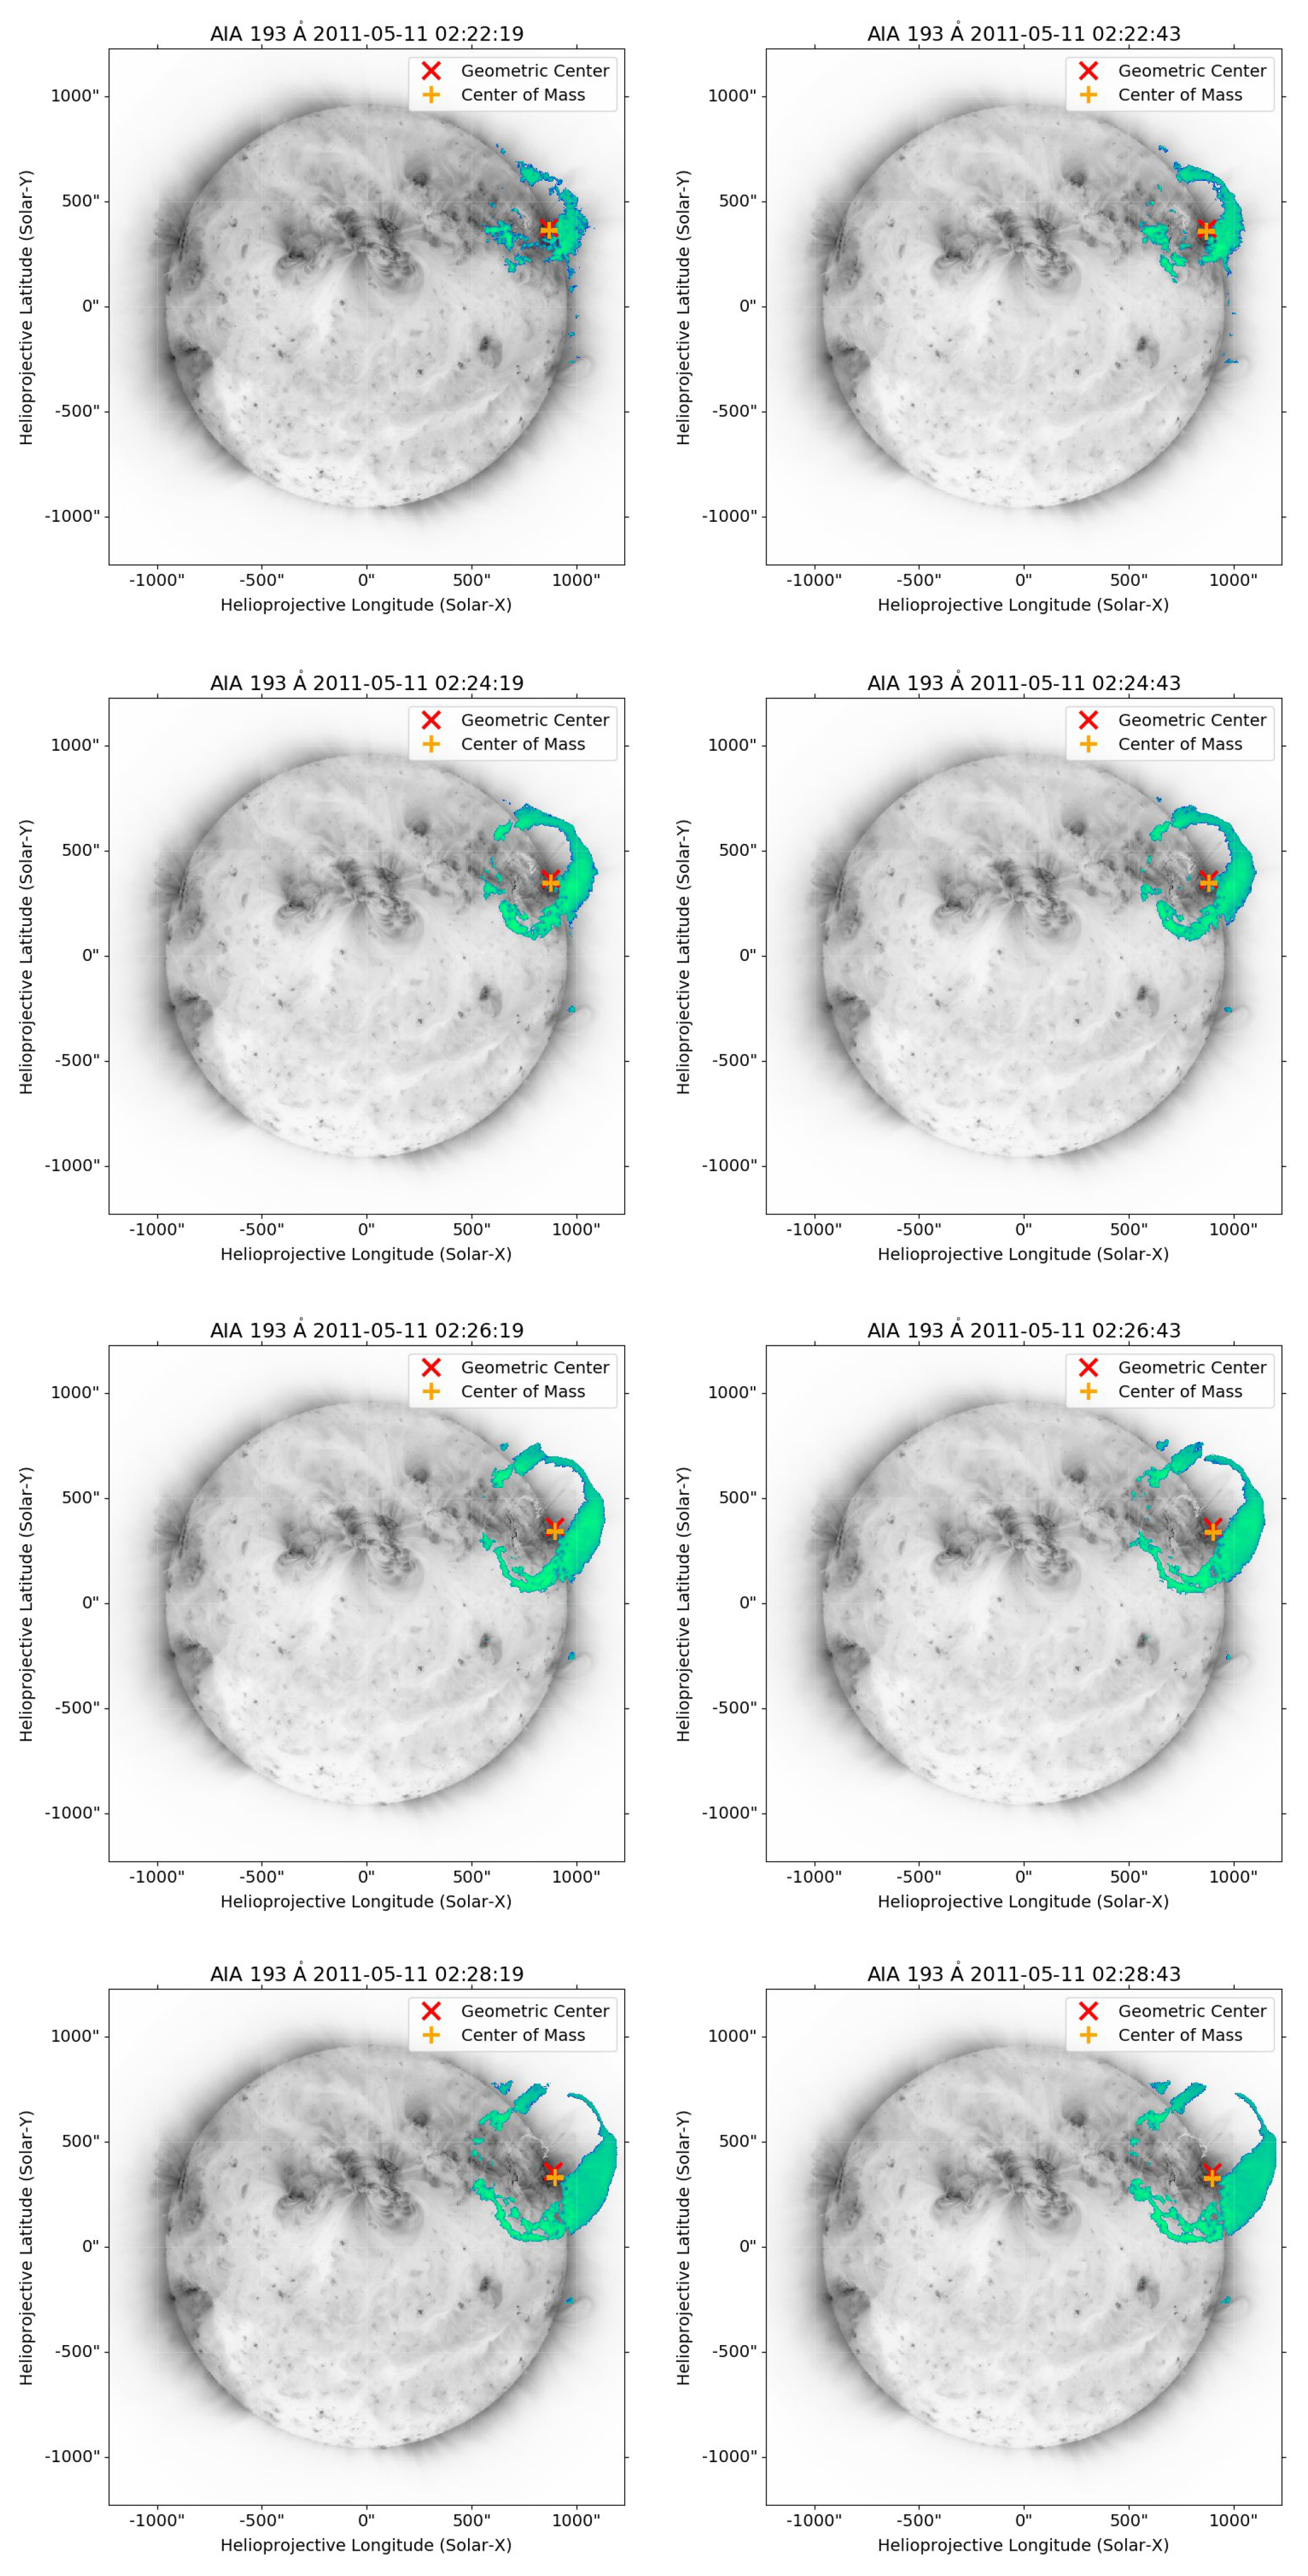
\includegraphics[width=0.7\hsize]{chapter2/figs/wavetrack_figure_110511.png}
	\caption{Wavetrack images of a May 11, 2011 eruption, with CBF mask applied. Four image pairs shown, separated by 2 minutes, to track CBF over time. Credit goes to \citet{stepanyuk_2022}.}
	\label{fig_wavetrack_cbf_center}
\end{figure}

Focusing on the May 11, 2011 event accompanied by a CBF, the methodology was applied to three events observed by AIA \citep{kozarev_2015, kozarev_2017}. Wavetrack adeptly tracked CBF evolution both on the solar disk and off the limb, maintaining performance despite pixel distribution and intensity differences.
The application facilitated detailed study of CBF shapes and intensity distributions, separate from the broader corona. Wavetrack effectively segmented CBF objects under different activity states, highlighting its capability to track multiple separate parts of the same feature.

Wavetrack was used to isolate and study CBF and filament kinematics using the FLCT method. Figure~\ref{fig_wavetrack_cbf_center} shows FLCT results of the May 11, 2011 event, revealing uneven expansion of the CBF from the central source. The combined approach elucidated dynamic behavior not discernible from intensity observations alone.
Figure~\ref{fig_flct_110511} displays the direction and speed of each CBF region. It reveals uneven expansion, with the thinnest part, strongly driven by the erupting filament, moving fastest. This nuanced insight, inaccessible through intensity observations alone, highlights the value of our combined Wavetrack and FLCT approach in understanding coronal feature dynamics.
Figure~\ref{fig_wavetrack_center_of_mass} depicts thorough analysis of CBF centers of mass (CM) and geometric centers (GC), illustrating their positional and speed variations over time. These findings provide valuable insights into CBF dynamics during the specified event.

\begin{figure}[!htp]
	\centering
	\includegraphics[width=0.7\hsize]{chapter2/figs/flct_wave_filament_doubleplot_figure_110511.png}
	\caption{FLCT model output for four image pairs from Fig. 3. Left: the plane-of-sky velocity vectors. Right: plane-of-sky speed. Credit goes to \citet{stepanyuk_2022}.}
	\label{fig_flct_110511}
\end{figure}

\begin{figure}[!htp]
	\centering
	\includegraphics[width=0.7\hsize]{chapter2/figs/event_110511_01_centers_of_mass.png}
	\caption{Analysis of the center of mass and geometric centers' motion during the May 11, 2011 event. The different rows present the X-, Y-, and R- positions for both GC and CM, the distance between GC and CM in \textit{km}, and the angle between these two points over time. Credit goes to \citet{stepanyuk_2022}.}
	\label{fig_wavetrack_center_of_mass}
\end{figure}

%%%%%%%%%%%%%%%%%%%%%%%%%%%%%%%%%%%%%%%%%%%%%%%%%%%%%%%%%%%%%%%%%%%%%%%%%%%%%%%%

\section{Geomagnetic Storms: CME Speed De-Projection vs. In Situ Analysis}
This study, led by \citet{miteva_2023}, examines the relationship between geomagnetic storm (GS) intensity and solar/interplanetary phenomena. Using the \textit{PyThea} framework, we reconstruct 3D geometry of geo-effective CMEs and compare on-sky and de-projected speed values, employing spheroid, ellipsoid, and graduated cylindrical shell (GCS) models. We investigate parameters of GS-associated phenomena, finding that fast CME speeds combined with specific magnetic structure orientations are indicative of GS strength. Accurate estimations of geometry, direction, and de-projected speeds are crucial for GS forecasting in space weather prediction schemes.

\subsection{Overview}
Solar eruptive events such as CMEs and solar flares (SFs) influence space weather, with electromagnetic radiation preceding energetic particles and CME plasma clouds \citep{fletcher_2011, webb_2012, klein_2017, temmer_2021, malandraki_2018, gopalswamy_sun_sw_2022}. Geomagnetic storms (GSs) occur due to interactions between solar wind plasma and Earth's magnetosphere, facilitated by magnetic reconnection during events like CME impacts \citep{dungey_1961, akasofu_1981, echer_2022, gonzalez_1994, saiz_2013, lakhina_2016}. Fast CMEs cause intense GSs, affecting technology and inducing disruptions in near-Earth space \citep{tsurutani_1997, zhang_2007, wu_2016, borovsky_2006, pulkkinen_2007}.

However, single spacecraft observations limit accurate CME speed estimations due to projection effects \citep{paouris_2021, kouloumvakos_2022}. Previous studies found no clear correlation between GS intensity and solar flare/CME parameters \citep{samwel_2023}, highlighting the need for reliable early warnings based on solar or near-Sun measurements. Accurate prediction of CME impact on Earth requires understanding their directionality and geometry, crucial for maximizing forecast lead time \citep{kay_2018, vourlidas_2003, jackson_2010}.

Improving reconstruction techniques to correct projection effects enhances CME propagation understanding and forecasting \citep{thernisien_2009, mierla_2010, wood_2010, thernisien_2011}. Existing CME propagation models exhibit discrepancies between 2D and 3D speeds and widths \citep{odstrcil_2004, xie_2004, vrvsnak_2013, pomoell_2018, jang_2016, verbeke_2022}. This study focuses on deducing CME directionality and near-Sun speeds using the PyThea framework \citep{kouloumvakos_2022}, analyzing geo-effective cycle 24 CMEs and their correlations with GS intensity and interplanetary parameters.

The event selection process identified 25 significant GSs within Solar Cycle 24 (SC24) and associated them with potential IP and/or solar phenomena. This involved temporal associations with IP and ICME events, CMEs, and solar flares. Various databases and catalogs were utilized for this analysis \citep{gonzalez_1994, gopalswamy_gs_2022, qiu_2022, besliu_2022, abe_2023, zhang_2007, gonzalez_2007, gopalswamy_2008, echer_2013, manu_2022}.

Utilized databases and catalogs include the GS database Kyoto\footnote{\url{https://wdc.kugi.kyoto-u.ac.jp/dstdir/index.html}}, SF database (GOES)\footnote{\url{http://ftp.swpc.noaa.gov/pub/warehouse/}}, CME catalog (SOHO-LASCO)\footnote{LASCO CME Catalog: \url{https://cdaw.gsfc.nasa.gov/CME_list/}}, ICME Wind and ACE databases\footnote{\url{https://wind.nasa.gov/ICME_catalog/ICME_catalog_viewer.php}},\footnote{\url{https://izw1.caltech.edu/ACE/ASC/DATA/level3/icmetable2.htm}}, and IP shock database (Wind)\footnote{\url{http://www.ipshocks.fi/database}},\footnote{\url{https://lweb.cfa.harvard.edu/shocks/wi_data/}}. These resources were accessed for relevant data retrieval and analysis \citep{selvakumaran_2016}.

\subsection{PyThea 3D De-Projection Tool}
This investigation employs the PyThea online tool for 3D reconstruction of CMEs and shock waves \citep{kouloumvakos_2022}, utilizing spheroid, ellipsoid, and GCS models. Two independent observers conduct fitting procedures. Figure~\ref{fig_3D_fit} illustrates fits for event E03, revealing observer bias in structure alignment with the model, potentially leading to CME width overestimation. However, despite this bias, overall results for event E03, including directivity and speed, remain minimally impacted, though discrepancies may arise among different observers.

\begin{figure}[!htp]
	\centering
	\begin{subfigure}[b]{0.3\textwidth}
		\includegraphics[width=\textwidth]{chapter2/figs/Fig_s1.png}
	\end{subfigure}
	\hfill
	\begin{subfigure}[b]{0.3\textwidth}
		\includegraphics[width=\textwidth]{chapter2/figs/Fig_e1.png}
	\end{subfigure}
	\hfill
	\begin{subfigure}[b]{0.3\textwidth}
		\includegraphics[width=\textwidth]{chapter2/figs/Fig_g1.png}
	\end{subfigure}
	\medskip % Add some vertical space between rows
	\begin{subfigure}[b]{0.3\textwidth}
		\includegraphics[width=\textwidth]{chapter2/figs/Fig_s2.png}
	\end{subfigure}
	\hfill
	\begin{subfigure}[b]{0.3\textwidth}
		\includegraphics[width=\textwidth]{chapter2/figs/Fig_e2.png}
	\end{subfigure}
	\hfill
	\begin{subfigure}[b]{0.3\textwidth}
		\includegraphics[width=\textwidth]{chapter2/figs/Fig_g2.png}
	\end{subfigure}
	\caption{3D reconstructions of a CME (E03) using the spheroid, ellipsoid, and GCS model from the PyThea tool performed by observers 1 and 2 (top and bottom row, respectively). Credit goes to \citet{miteva_2023}.}
	\label{fig_3D_fit}
\end{figure}

In five cases (E05, E11, E17, E18, E22), attempts to identify SFs or CMEs were unsuccessful, while in six additional cases, SF specifications were unattainable. Events with uncertain CME origins were excluded from subsequent 3D analyses. For example, the unique orientation of a double CME in case E07 rendered its de-projection unfeasible, leading to its exclusion. Similarly, in seven cases (E12, E14–E16, E19, E23, E25), data retrieval issues from both spacecraft led to their omission from 3D analyses.

The study focuses on deriving de-projected CME speeds based on fits at two distinct time steps. Initial CME longitude and latitude are manually specified for each model, utilizing provided SF locations. Final CME directivity is considered relatively crude, derived from qualitative information extracted from available animations\footnote{\helioweatherurl}. This approach ensures a rigorous basis for evaluating de-projected CME speeds.

\subsection{Results}
\subsubsection{Projection Effects}
Approximately 10 CMEs were analyzed by two designated observers in our research team, including myself, utilizing all three models in the PyThea framework. The fitting process involved two time steps to derive velocity parameters based on height–time estimations. Both observers conducted the 3D de-projection procedure iteratively for each event, resulting in averaged CME speeds presented in Table~\ref{tab_fits}, rounded to the nearest tenth. Discrepancies between fitting instances were treated as errors, ranging from 10 \kms to twice the estimated speed. Figure~\ref{fig_vcme_err} illustrates the correlation between 3D speeds and estimated errors, showing significant variability, particularly with the GCS model, but a discernible positive trend between error magnitude and CME speed.

Subjectivity and varied experience levels among observers influenced the visual fitting process, leading to differences in evaluated speeds, both within individual observers using the same model and across different models for a single observer. Variations in operating system software also contributed to result discrepancies. Events E04, E08, and E21 were incomplete due to PyThea computing issues or substantial uncertainty in CME structure assessment.

Our findings highlight the inherent subjectivity in procedures relying on personal judgment for fit quality, detailed further in \citep{verbeke_2022}. Averaged CME speeds, meticulously outlined in Table~\ref{tab_fits}, will serve as the basis for subsequent correlation studies.

\begin{table}[!htp]
	\caption{CME Speeds (\kms) for Observers 1 and 2. Credit goes to \citet{miteva_2023}.}
	\label{tab_fits}
	\centering
	\begin{tabular}{ccccccc}
		\toprule
		\textbf{\#} & \multicolumn{2}{c}{\textbf{Spheroid}} & \multicolumn{2}{c}{\textbf{Ellipsoid}} & \multicolumn{2}{c}{\textbf{GCS}} \\
		& \textbf{obs1} & \textbf{obs2} & \textbf{obs1} & \textbf{obs2} & \textbf{obs1} & \textbf{obs2} \\
		\midrule
		E01 & $2170\pm870$ & $1800\pm270$ & $2130\pm200$ & $1710\pm450$ & $1590\pm100$ & $1760\pm10$ \\
		E02 & $1780\pm140$ & $1350\pm50$  & $1880\pm580$ & $1310\pm90$ & $1780\pm260$ & $1630\pm130$ \\
		E03 & $770\pm40$ & $740\pm10$ & $640\pm180$ & $740\pm180$ & $1020\pm170$ & $700\pm270$ \\
		E04 & - & $2150\pm140$ & - & $2460\pm70$ & - & $2530\pm630$ \\
		E06 & $1410\pm420$ & $710\pm70$ & $1870\pm50$ & $1700\pm300$ & $1680\pm870$ & $1560\pm470$ \\
		E08 & $350\pm90$ & - & $360\pm150$  & - & $350\pm70$ & - \\
		E09 & $690\pm280$ & $630\pm150$ & $550\pm170$  & $590\pm60$ & $670\pm610$ & $710\pm220$ \\
		E10 & $840\pm380$ & $610\pm1040$ & $1120\pm360$ & $960\pm90$ & $1160\pm650$ & $1310\pm80$ \\
		E13 & $320\pm90$ & $350\pm50$ & $620\pm140$ & $750\pm160$ & $780\pm80$ & $1310\pm700$ \\
		E20 & $830\pm190$ & $800\pm600$ & $790\pm90$ & $570\pm20$ & $1240\pm280$ & $1130\pm230$ \\
		E21 & $620\pm230$ & - & $440\pm40$ & - & $280\pm180$ & - \\
		E24 & $750\pm270$ & $1310\pm220$ & $880\pm350$ & $2020\pm960$ & $950\pm120$ & $1560\pm540$ \\
		\bottomrule
	\end{tabular}
\end{table}

\begin{figure}[!htp]
	\centering
	\includegraphics[width=0.48\hsize]{chapter2/figs/Fig_er_speed1.pdf}
	\includegraphics[width=0.48\hsize]{chapter2/figs/Fig_er_speed2.pdf}
	\caption{Scatter plot illustrates the comparison of 3D de-projected CME speeds derived from the spheroid model (depicted as diamonds), the ellipsoid model (represented by stars), and the GCS model (indicated as dots) versus the measurement errors for observers 1 (left) and 2 (right). Credit goes to \citet{miteva_2023}.}
	\label{fig_vcme_err}
\end{figure}

\subsubsection{Correlation between GSs, Coronal, and Near-Sun Parameters}
Figure~\ref{fig_speeds_dst} shows a scatter plot illustrating the relationship between the modulus of the GS Dst index and CME speed. Averaged results of three model fits (\textit{3D-mean}) are compared with 2D SOHO-LASCO CME speeds in Table~\ref{tab_cc_CME}, alongside error estimates from 3D de-projections. Despite some overlap, the largest error value among observers (as outlined in Table~\ref{tab_fits}) is highlighted for clarity.

Analysis reveals no discernible trend between the Dst index and CME speed, regardless of considering 3D de-projections or 2D CME speeds. Data constraints prevented 3D speed de-projections for the most robust GSs, skewing speed distribution and impacting findings. Despite the modest sample size (10 to 20 event pairs), Pearson correlations assess fit quality. Coefficients in Table~\ref{tab_cc_CME} range from negligible (e.g., 0.04 for 2D LASCO speeds) to moderate (highest: 0.55 with GCS model). Notably, no significant correlations are found between Dst index and other coronal parameters (e.g., SF class, location, CME AW), as comprehensively presented in the same table.

\begin{table}[!htp] 
	\small
	\centering
	\caption{Table displaying Pearson correlation coefficients among the GS Dst index, CME speed, and various solar parameters, with the respective sample sizes indicated in parentheses. Credit goes to \citet{miteva_2023}.}
	\label{tab_cc_CME}
	\begin{tabular}{llll}
		\toprule
		\textbf{CME source}	& \textbf{Dst$-$speed} & \textbf{solar parameter} & \textbf{Dst$-$solar parameter}	\\
		\midrule
		LASCO              & 0.04 (20) & SF class      & $-$0.04 (14) \\
		{\bf 3D - mean}    & {\bf 0.49 (12)} & SF latitude   & $-$0.16 (14)   \\
		3D spheroid - mean & 0.34 (12) & SF longitude  & 0.13 (14)	\\
		3D spheroid - obs1 & 0.14 (11) & CME AW        & 0.03 (20) \\
		3D spheroid - obs2 & 0.15 (10) & \\ 
		3D ellipsoid - mean & 0.53 (12) & &	\\
		3D ellipsoid - obs1 & 0.28 (11) & & \\
		3D ellipsoid - obs2 & 0.40 (10) & &\\
		3D GCS - mean & 0.55 (12) & &\\
		3D GCS - obs1 & 0.49 (11) & &\\
		3D GCS - obs2 & 0.27 (10) & & \\
		\bottomrule
	\end{tabular}
\end{table}

\begin{figure}[!htp]
	\centering
	\includegraphics[width=0.7\hsize]{chapter2/figs/Fig_GS_speed_er_mean.pdf}
	\caption{Scatter plot illustrating the relationship between the Dst index and CME speed, incorporating data from the SOHO/LASCO instrument (represented by filled circles) and 3D de-projections (depicted by empty circles). Credit goes to \citet{miteva_2023}.}
	\label{fig_speeds_dst}
\end{figure}

\begin{figure}[!htp]
	\centering
	\begin{subfigure}[b]{0.45\textwidth}
		\includegraphics[width=\textwidth]{chapter2/figs/Fig_GS_ICMEspeed.pdf}
	\end{subfigure}
	\hfill
	\begin{subfigure}[b]{0.45\textwidth}
		\includegraphics[width=\textwidth]{chapter2/figs/Fig_GS_IPspeed.pdf}
	\end{subfigure}
	\begin{subfigure}[b]{0.45\textwidth}
		\includegraphics[width=\textwidth]{chapter2/figs/Fig_GS_Ms.pdf}
	\end{subfigure}
	\hfill
	\begin{subfigure}[b]{0.45\textwidth}
		\includegraphics[width=\textwidth]{chapter2/figs/Fig_GS_sheath.pdf}
	\end{subfigure}
	\begin{subfigure}[b]{0.45\textwidth}
		\includegraphics[width=\textwidth]{chapter2/figs/Fig_GS_Bz.pdf}
	\end{subfigure}
	\hfill
	\begin{subfigure}[b]{0.45\textwidth}
		\includegraphics[width=\textwidth]{chapter2/figs/Fig_GS_Bjump.pdf}
	\end{subfigure}
	\begin{subfigure}[b]{0.45\textwidth}
	\includegraphics[width=\textwidth]{chapter2/figs/Fig_GS_Tjump.pdf}
\end{subfigure}
	\hfill
\begin{subfigure}[b]{0.45\textwidth}
	\includegraphics[width=\textwidth]{chapter2/figs/Fig_GS_Njump.pdf}
\end{subfigure}
	\caption{Comprehensive scatter plots illustrating the relationships between Dst index and various solar wind parameters, including Wind/ACE ICME speed, IP shock speed, Mach number, duration of sheath region, Bz, magnetic field jump, temperature jump, and density jump. Credit goes to \citet{miteva_2023}.}
	\label{fig_dst_scatterplots}
\end{figure}

\begin{table}[!htp] 
	\small
	\centering
	\caption{Tabular representation of Pearson correlation coefficients between the GS Dst index and various parameters of IP phenomena. The data is derived from Wind satellite measurements, unless otherwise stated, with the corresponding sample sizes indicated in parentheses. Credit goes to \citet{miteva_2023}.}
	\label{tab_cc_IP}
	\begin{tabular}{lc}
		\toprule
		\textbf{IP parameter} & \textbf{Dst$-$IP parameter} \\
		\midrule
		ICME speed  & 0.37 (24)	\\
		ICME speed (ACE)   & 0.44 (22)	\\
		IP shock speed  & 0.35 (22)	\\
		Mach number  & 0.36 (21)	\\ 
		sheath duration & 0.22 (20) \\
		$|B_z|$      & 0.37 (25) \\
		$B_d/B_u$  & 0.48 (21)	\\
		$T_d/T_u$  & 0.40 (21)	\\
		$N_d/N_u$  & 0.46 (21)	\\
		{\bf $B$}  & {\bf $-$0.14 (20)}  \\
		{\bf $V$}       & {\bf 0.19 (20)}	\\
		{\bf $\beta_u$} & {\bf $-$0.14 (21)}	\\
		\bottomrule
	\end{tabular}
\end{table}

\subsubsection{Correlation between GSs and IP Parameters}
We explore correlations between GSs and various parameters linked to pre-selected IP phenomena. Scatter plots illustrate relationships such as Dst index versus ICME speed and IP shock speed, Dst versus Mach number and sheath duration, and Dst versus $|Bz|$ and $B_d/B_u$. Figure~\ref{fig_dst_scatterplots} and Table~\ref{tab_cc_IP} detail these correlations.
For the limited sample used, we observe moderately positive trends between Dst index and plasma compression parameters at the shock interface, comparable to or slightly larger than correlations with ICME speeds. However, the trend with $|Bz|$ is weaker (0.37), contrasting with robust trends from prior studies. Correlations involving Dst and IP shock speed, Mach number, or sheath duration are relatively smaller.

Recent reports suggest strong correlations with electric and magnetic field components \citep{echer_2022}, although this exceeds our current analysis scope. Caution is warranted in interpreting results due to lack of uncertainty estimates for correlation coefficients. Additional parameters from ICME and IP shock catalogs show no robust correlations with Dst index, all correlation coefficients being smaller than 0.2.

\subsubsection{Forecasting GS Strength Based on Solar and IP Parameters}
We examine how magnetic obstacle type, orientation upon Earth arrival, and 3D reconstructed CME speeds collectively impact GS intensity, approximated by the Dst index.

The most potent GSs in our compilation exhibit distinctive magnetic structure parameters, including complexity, orientation, and speed at Earth. Exceptions include instances of fast speed flank hits or uncertain configurations, possibly influenced by fast solar wind streams or CIRs. Notably, IP structure associated with certain GSs has notably low speeds.
Interpretation considers information from both speed reconstructions and in situ measurements to enhance analysis robustness.

\section{Discussion}
The May 11, 2011 eruption showcased a variety of solar phenomena, including a fast partial-halo CME, a weak solar flare, an eruptive filament, and a type II radio burst. Analyzing the interplay of these events offers insights into solar and interplanetary dynamics.

\subsection{CME Kinematics and Coronal Shock Wave Characteristics}
The CME exhibited characteristics such as a linear speed of 745 \kms, an acceleration of 3.3 m s$^{-2}$, and an angular width of 225\degree. The associated shock wave displayed complex kinematics, observed in both the low and middle/outer corona.

In the low corona, the shock wave's asymmetry and evolving geometry revealed dynamic behavior. Differences in thickness, speed, and acceleration between flanks suggested complex interactions with the coronal environment. Segmenting the shock surface highlighted variations in shock characteristics.

In the middle/outer corona, SOHO/LASCO measurements depicted the dynamic evolution of the EUV wave. Gallagher model fitting emphasized the importance of combining AIA and LASCO measurements. Fluctuations in acceleration and speed underscored the shock wave's complexity.

Statistical analysis revealed patterns in coronal wave events, with radial waves exhibiting distinct characteristics compared to lateral waves. Cumulative dynamic spectra illustrated trends in shock speed and intensity with distance.
Correlations between plasma parameters and shock characteristics were identified, laying the groundwork for further parameterizations in subsequent phases of the project.

\subsection{Dynamic Coronal Features Analysis with Wavetrack}
\citet{stepanyuk_2022} utilized Wavetrack to study eruptive solar events, focusing on the May 11, 2011 event associated with a significant CBF. Two additional events, on June 7, 2011, and December 12, 2013, were also examined, demonstrating Wavetrack's versatility in tracking various solar features.

Wavetrack efficiently delineated evolving CBFs across consecutive time steps, even with variations in pixel distributions and intensities. This enabled detailed exploration of time-dependent shapes and intensity distributions, distinct from the broader corona. Segmentation during the December 12, 2013 event highlighted Wavetrack's effectiveness in tracking multiple parts of the same feature.

To analyze CBF and filament kinematics, the FLCT method was employed. Results revealed the plane-of-sky direction and speed of different CBF regions during the May 11, 2011 event. The study showcased the complementary nature of Wavetrack and FLCT in elucidating dynamic behavior.

The study calculated plane-of-sky speeds of the erupting filament driver (Fig.~\ref{fig_flct_110511}), showing higher speeds directly below the region of highest speeds in the CBF. Geometric centers and centers of mass were determined, providing insights into the dynamics of the solar eruption event.
These findings offer insights into the dynamics and characteristics of the May 11, 2011 solar eruption event, particularly regarding the movement and speeds of key features like the CBF and erupting filament driver.

\subsection{Subjectivity in CME Speed Determination}
Our study on CMEs reveals significant variability due to subjectivity in fitting and de-projection procedures. Analysis of approximately 10 CMEs using PyThea framework models highlights observer disparities and technical limitations. Averaged CME speeds, documented in Table~\ref{tab_fits}, show associated errors emphasizing the challenges and uncertainties in this process.

Despite subjectivity challenges, these averaged values form the basis for correlation studies. Correlating GSs with parameters like the Dst index and CME speeds reveals no discernible trend, with Pearson correlation coefficients indicating diverse relationships.

Scatter plots in Figure~\ref{fig_dst_scatterplots} and Table~\ref{tab_cc_IP} show moderately positive correlations between the Dst index and plasma compression parameters at the shock interface. However, caution is warranted due to the absence of uncertainty estimates for correlation coefficients.

Further analysis of magnetic obstacle characteristics and 3D CME speeds sheds light on patterns influencing GS intensity. Nose-like orientation and complex or flux-rope structures characterize the most potent GSs. Limitations in single-point IP shock speed measurements underscore the need for comprehensive interpretation considering both speed reconstructions and in situ measurements.

\section{Conclusions}
I conducted a study characterizing 26 historical CME-driven CBFs in the low solar corona, observed with the AIA instrument onboard the SDO spacecraft. Utilizing the SPREAdFAST framework, we integrated physics-based and data-driven models to estimate coronal magnetic fields, shock wave dynamics, energetic particle acceleration, and SEP propagation. The analysis relied on AIA base-difference images to generate annulus plots and J-maps for kinematic measurements in radial and lateral directions.

Various time-dependent and distance-dependent kinematic parameters were computed, including shock speed, acceleration, intensity, and thickness. LASCO measurements up to 17$R_{\odot}$ were incorporated to improve SEP spectra characterization. Kinematic measurements facilitated time-dependent 3D geometric models of wavefronts and informed plasma diagnostics through MHD and DEM models.

Shock kinematic measurements were used to fit geometric spheroid surface models for each time step, capturing shock characteristics accurately. Parametrized relationships between plasma parameters were explored to identify connections and interdependencies.

In \citet{stepanyuk_2022}, we present Wavetrack, an innovative method for automated identification and monitoring of dynamic coronal phenomena. By employing wavelet decomposition, feature enhancement, and filtering, Wavetrack generates time-dependent masks for feature pixels, particularly adept at tracing faint, large-scale features like coronal bright fronts (CBFs) and EUV waves. Operable for on-disk and off-limb features, Wavetrack is implemented as a versatile Python framework.

Application to four events, focusing on CBFs in May 11 and June 07, 2011, and December 12, 2013, demonstrates Wavetrack's proficiency in tracking complete CBF pixel maps. Integrating with the FLCT method reveals the dynamic evolution of CBF regions and their correlation with eruptive filament drivers, highlighting compression effects and speed variations.

Wavetrack also tracks temporal changes in feature regions by computing time-dependent vectors between pixel geometric centers and centers of mass, providing valuable metrics for feature evolution. However, manual segmentation and parameter fine-tuning are currently required, with plans for future improvements to enhance versatility.

The methodology shows promise for broader application across solar dynamic features and datasets, with future research extending its use to filament evolution and coronagraph data analysis, refining our understanding of eruptive front variations across different observational contexts.

Our findings in \citet{kozarev_2022} and \citet{stepanyuk_2022} contribute to understanding shock kinematics and plasma parameters. Future investigations will focus on SEP acceleration near the Sun and transport of coronal and interplanetary particles, refining shock and coronal parameter characterization methods for enhanced accuracy and reliability.

In \citet{miteva_2023}, we analyze geo-effective storms during solar cycle 24 to identify predictors for storm intensity. Our approach integrates solar, near-Sun, and interplanetary parameters, incorporating results from PyThea, a tool for CME speed de-projection. We find improvements in correlation coefficients for projected CME speed, although fast CMEs pose challenges due to reconstruction errors and structural complexity.

Fast halo CMEs exhibit significant deviations, affecting reconstruction quality and limiting forecasting potential for storm strength. In contrast, certain interplanetary parameters, particularly ICME and IP shock speeds, show moderate positive correlations with storm intensity. However, discrepancies in measurements and single-point observations raise concerns about predictive capability.

Among various parameters, the combination of speed and orientation of the magnetic obstacle appears influential, as seen qualitatively in the \textit{helioweather} animations. While de-projected CME speeds enhance modeling accuracy, they do not directly impact storm intensity. Permanent stereoscopic observations, like the ESA Vigil mission, are crucial for improved 3D reconstructions of CME geometries and accurate speed estimations.

In conclusion, our study lays the groundwork for ongoing projects aimed at refining parameterizations and integrating synoptic MHD parameters into the \textit{S3M} synoptic model, enhancing our understanding of solar dynamics and space weather forecasting.

Our findings highlight the importance of integrating advanced tracking methodologies like Wavetrack with kinematic analyses such as FLCT, providing deeper insights into the complexities of eruptive solar events. As we refine these methodologies, our understanding of solar phenomena will advance, contributing to Heliophysics.
Furthermore, our study emphasizes the complexity of studying CMEs and their impact on geomagnetic storms. Integrating observational data and model outputs offers a comprehensive perspective for further investigations into the dynamic interplay between solar and interplanetary phenomena in shaping space weather events.

\chapter{Modeling and Foreasting Solar Energetic Protons (SEP)}
\label{chapter3}

\section{Introduction}

\section{Data preparation}

\section{Method}

\subsection{The Bi-LSTM Model}

\subsection{Model selection}


\section{Results and discussion}

\section{Conclusions}



\chapter{Modeling and Forecasting of Solar Energetic Protons (SEP)}
\label{chapter4}
This chapter has two parts. In the first part, I describe a modeling study that we conducted on energetic proton acceleration and propagation from the solar corona to 1 AU. For this modeling, we employ the physics-based approach utilized in the first chapter, including the 3D coronal models and a 3D MAS-MHD model run. With these models, we use the EPREM model to find the fluxes and spectra of energetic protons at 1 AU. We then compare the modeling results with in-situ measurements. In the second part, I describe a deep learning approach that I developed to forecast the integral flux of energetic protons in three energy channels across three different forecasting horizons.

\section{Introduction}
\label{sec_ch4_intro}
Coronal Mass Ejections (CMEs) represent significant phenomena in solar physics, captivating attention due to their prominent role in solar activity. Traditionally, CMEs have been identified through white light observations, providing valuable insights into their characteristics \citep{vourlidas_2003, zhang_2006, bein_2011}. However, a comprehensive understanding of these eruptions requires examination across multiple wavelengths, including ultraviolet and radio bands, where observations reveal additional facets of their dynamics \citep{bastian_2001, veronig_2010}. Notably, extreme ultraviolet (EUV) observations, facilitated by instruments like the Atmospheric Imaging Assembly (AIA) on the Solar Dynamics Observatory, have become instrumental in capturing the early stages of CMEs \citep{lemen_2012, pesnell_2012}.

CMEs, in their trajectory through the solar corona, can give rise to shock waves when their propagation speeds surpass the local fast magnetosonic speed, observable as EUV waves or coronal bright fronts (CBFs) \citep{thompson_1998, long_2011}. These shock waves are crucial in the context of Solar Energetic Particle (SEP) acceleration. While solar flares also contribute to SEP production, recent advancements in observations and numerical modeling have reshaped the prevailing understanding. It is now recognized that, especially in their early stages (below 5–10\rsun), CMEs often drive shocks capable of accelerating SEPs to energies exceeding 100 MeV/n \citep{ontiveross_2009, gopalswamy_2011, battarbee_2013, kozarev_2013, schwadron_2014, kong_2017}.

Previous research has primarily focused on characterizing the dynamics of CMEs and their associated shocks within the solar corona, utilizing advanced observations spanning white light, EUV, and radio wavelengths \citep{vourlidas_2003, zhang_2006, bein_2011}. The relationship between CMEs and shock waves, particularly coronal bright fronts (CBFs), has been a subject of in-depth investigation. Notably, \citet{kozarev_2019} conducted a comprehensive study of nine distinct western CBF events, employing the Diffusive Shock Acceleration (DSA) model proposed by \citet{kozarev_2016}. Their findings revealed variations in SEP production among events, coupled with evolving patterns over the course of each event. Moreover, the acceleration efficiency demonstrated a strong dependence on the diverse coronal environments traversed by the propagating shock waves.

Building upon the groundwork laid by \citet{kozarev_2019}, this present study extends its scope by modeling the dynamics of CBF-related shock/compression waves and particle acceleration up to 10\rsun. This advancement involves integrating outcomes with a comprehensive numerical particle transport model, allowing for comparisons with in situ observations. This marks a significant enhancement in our methodology, representing the first validated extension of Sun-to-Earth physics-based modeling for SEP acceleration and transport within our current understanding of solar physics \citep{kozarev_2022}.

In the quest to understand the mechanisms through which Solar Energetic Particles (SEPs) are produced by coronal shocks throughout the inner heliosphere, considerable progress has been made. Traditionally, the prevailing assumption was that SEP acceleration primarily occurred in interplanetary space, driven by in situ measurements of Energetic Storm Particle (ESP) fluxes during encounters with interplanetary shocks by spacecraft. However, recent advancements in observations and numerical modeling have reshaped this understanding.

CMEs emerge as the principal contributors to the generation of SEPs, encompassing ions and electrons with energies several orders of magnitude beyond the thermal coronal plasma \citep{reames_1999}. While solar flares also contribute to SEP production during solar eruptions, CMEs predominantly facilitate SEP generation within the magnetized shock waves they instigate and in plasma compressions resulting from their expansive forces. The prevailing assumption that the majority of SEP acceleration transpired in interplanetary space has been challenged by the revelation that, particularly in their initial stages (below 5–10\rsun), CMEs frequently induce shocks capable of accelerating SEPs to energies surpassing 100 MeV/n \citep{ontiveross_2009, gopalswamy_2011, battarbee_2013, kozarev_2013, schwadron_2014, kong_2017}.

Efforts have been directed towards characterizing the dynamics of CMEs and the accompanying shocks within the solar corona, employing increasingly sophisticated observations spanning white light, EUV, and radio wavelengths. This exploration aims to deduce early-stage SEP production in the solar corona \citep{kozarev_2013, schwadron_2015}. In a notable contribution, \citet{kozarev_2019} conducted an in-depth study of nine distinct western CBF events, utilizing the Diffusive Shock Acceleration (DSA) model proposed by \citet{kozarev_2016}. Their findings highlighted variations in SEP production among events, along with evolving patterns over the duration of each event. Importantly, the acceleration efficiency exhibited a strong dependence on the diverse coronal environments traversed by the propagating shock waves.

This study, led by \citet{kozarev_2022}, advances the work of \citet{kozarev_2019} by extending the modeling of CBF-related shock/compression wave dynamics and particle acceleration to 10\rsun. Our approach involves coupling these results with a global numerical particle transport model and comparing the outcomes to in situ observations. This represents a significant enhancement in our methodology, marking the first validated extension of Sun-to-Earth physics-based modeling for SEP acceleration and transport within our current understanding of solar physics.








Several models are available, or under development, for forecasting SEP, which use diverse approaches and serve different objectives. These models comprise computationally complex physics-based models, quick and simple empirical models, Machine Learning (ML)-based models, and hybrid models that combine different approaches and produce different types of outputs, including deterministic, probabilistic, categorical, and binary. Deterministic models always generate the same output without any randomness or stochastic components, such as predicting the SEP flux at a specific moment or the arrival time of SEP. On the other hand, probabilistic models provide a probability value that reflects the likelihood of an SEP event occurring. However, replicating SEP fluxes at a specific time is still a significant challenge for current models.

An excellent review on SEP models and predictive efforts was recently published by \citet{whitman_2022}, which summarizes the majority of the existing models.
For instance, \citet{papaioannou_2022} introduced the Probabilistic Solar Particle Event Forecasting (PROSPER) model, which is incorporated into the Advanced Solar Particle Event Casting System (ASPECS)\footnote{ASPECS: \url{http://phobos-srv.space.noa.gr/}}. The PROSPER model utilizes a Bayesian approach and data-driven methodology to probabilistically predict SEP events for 3 integral energy channels $>$10, $>$30, and $>$100 MeV. The model's validation results indicate that the solar flare and CME modules have hit rates of 90\% and 100\%, respectively, while the combined flare and CME module has a hit rate of 100\%.
\citet{bruno_2021} developed an empirical model to predict the peak intensity and spectra of SEP at 1 AU between 10 and 130 MeV, using data from multiple spacecraft. The model is tested on 20 SEP events and shows good agreement with observed values. The spatial distribution of SEP intensities was reconstructed successfully, and they found a correlation between SEP intensities and CME speed.

\citet{hu_2017} extended the Particle Acceleration and Transport in the Heliosphere (PATH) model to study particle acceleration and transport at CME-driven shocks. They showed that the model can be used to obtain simultaneous calculations of SEP characteristics such as time-intensity profiles, instantaneous particle spectra, and particle pitch angle distributions at multiple heliospheric locations. Overall, results resemble closely those observed in situ near the Earth but also yield results at other places of interest, such as Mars, making it of particular interest to Mars missions.
SPREAdFAST \citep{kozarev_2017, kozarev_2022} is a physics-based, data-driven framework that utilizes EUV observations and models to simulate SEP fluxes at 1 AU and to estimate energetic particle acceleration and transport to various locations in the inner heliosphere. It generates time-dependent histograms and movies distributing them through an online catalog. The accuracy and efficiency of the model were encouraging, but the highest energy fluxes showed disagreement with in situ observations by the SOHO/ERNE instrument. However, the framework has great potential for space weather science and forecasting.

In \citet{aminalragia_2021}, they used neural networks to provide probabilities for the occurrence of SEP based on soft X-rays data from 1988 to 2013. They obtained $>$85\% for correct SEP occurrence predictions and $>$92\% for correct no-SEP predictions.
\citet{lavasa_2021} described a consistent approach to making a binary prediction of SEP events using ML and conventional statistical techniques. The study evaluated various ML models and concluded that random forests could be the best approach for an optimal sample comprising both flares and CMEs. The most important features for identifying SEP were found to be the CME speed, width, and flare soft X-ray fluence.
\citet{kasapis_2022} employed ML techniques to anticipate the occurrence of a SEP event in an active region that generates flares. They utilized the Space-Weather MDI Active Region Patches (SMARP) dataset, which comprises observations of solar magnetograms between June 1996 and August 2010. The SMARP dataset had a success rate of 72\% in accurately predicting whether an active region that produces a flare would result in a SEP event. Moreover, it provided a competitive lead time of 55.3 min in forecasting SEP events.

\citet{engell_2017} introduced the Space Radiation Intelligence System (SPRINTS), a technology that uses pre- and post-event data to forecast solar-driven events such as SEP. It integrates automatic detections and ML to produce forecasts. Results show that SPRINTS can predict SEP with an 56\% probability of detection and 34\% false alarm rate.
Nevertheless, the HESPERIA REleASE tools provide real-time predictions of the proton flux at L1 by using near-relativistic electrons as a warning for the later arrival of protons and have been set to operation \citep{malandraki_2018}. Historical data analysis indicates high prediction accuracy, with a low false alarm rate of approximately 30\% and a high probability of detection of 63\% \citep{malandraki_2018}.

Forecasting SEP is a critical task that serves operational needs and provides insight into the broader field of space weather science and heliophysics. As emphasized in previous works, a high precision forecasting model is urgently required to predict SEP flux within a period of time, given the risks associated with these events. This highlights the critical requirement for a dependable forecasting system that can mitigate the risks associated with SEP.

Scientists have been using physics-based and empirical models for decades to forecast SEP. However, these models have certain limitations. Physics-based models require accurate input data and underlying physical assumptions. In addition, the complexity of the physics involved and incorrect parameters may introduce uncertainties that can lead to inaccurate predictions.
On the other hand, empirical models rely on historical data to make predictions.
While they can be accurate sometimes, they may be unable to account for changes in physical conditions related to the acceleration and propagation of SEP, which can influence prediction accuracy.
ML models, however, provide a different approach to SEP forecasting. These models can analyze vast amounts of data, learning patterns from the data that are used, and connections that may not be obvious to experts. Additionally, ML models can adapt to changes in underlying physical conditions, resulting in more accurate predictions as more data is collected; they also provide relatively rapid forecasts, which allows for incorporation into a real-time forecasting workflow.

In the upcoming sections, I will explore the limitations in accuracy that arise from dealing with an imbalanced dataset and low-resolution data. Specifically, the presence of intrinsic outliers in the time series data pertaining to SEP flux poses a significant challenge in modeling. These outliers correspond to occurrences of SEP events and, consequently, have an impact on the accuracy of predictions. Notably, they often lead to an underestimation of the SEP fluxes, primarily due to the predominance of relatively low values throughout the majority of the time interval.

In the first part, we extend the work in Chapter 2 on the kinematics of CBFs and expand on previous relevant investigations by modeling CBF-related shocks and particle acceleration up to 10 solar radii. Our modeling approach incorporates coupling to a numerical model of particle transport throughout the heliosphere, with validation against in-situ spacecraft measurements. Our study implements, for the first time, an extensive physics-based model linking CME-driven shock acceleration with the propagation of SEPs from the Sun to Earth. In the second part, I present advanced deep learning models to forecast the daily integral flux of SEP over a 3-day forecasting window by using bi-directional long short-term memory (BiLSTM) neural networks, for 3 energy channels ($>$10, $>$30, and $>$60 MeV). Our models can forecast the time-dependent development of SEP events in different energy domains, which can be used to model the space radiation profiles using frameworks such as BRYNTRN \cite{wilson_1988} and GEANT4 \citep{truscott_2000}.
%I describe the data selection and pre-processing in Section~\ref{sec_ch4_data_prep}. I present an overview on the analysis methods and the models implemented in Section~\ref{sec_ch4_methods}. Then I show the forecasting results in Section~\ref{sec_ch4_results}. Finally the summary and implications are presented in Section~\ref{sec_ch4_conclusion}.

\section{Early-Stage SEP Acceleration by CME-Driven Shocks}
\subsection{Overview}
Coronal Mass Ejections (CMEs) stand out as one of the most prevalent expressions of solar activity, attracting considerable attention in solar physics. Traditionally defined through white light observations \citep{vourlidas_2003, zhang_2006, bein_2011}, these eruptions reveal diverse facets when examined across ultraviolet and radio bands \citep{bastian_2001, veronig_2010}. Particularly noteworthy is their observation in extreme ultraviolet (EUV) light, a realm where telescopes like the Atmospheric Imaging Assembly (AIA) on the Solar Dynamics Observatory \citep{lemen_2012, pesnell_2012} excel in capturing the early stages of CMEs.

CMEs, in their dynamic journey through the solar corona, can generate shock waves if their propagation speeds surpass the local speed of information, typically the fast magnetosonic speed. These shock waves manifest prominently in EUV observations as EUV waves or, more specifically, as coronal bright fronts (CBFs) \citep{thompson_1998, long_2011}. The intricate relationship between CMEs and these shock waves forms a crucial aspect of solar physics.

As the primary contributors to solar energetic particles (SEPs), CMEs play a pivotal role in the energization of ions and electrons to levels significantly exceeding the thermal coronal plasma \citep{reames_1999}. Flares also contribute to SEP production during solar eruptions. The acceleration of SEPs in CMEs predominantly occurs within the magnetized shock waves they propel, as well as in plasma compressions induced by the CMEs. While historical perspectives inferred the bulk of SEP acceleration in interplanetary space from in situ observations of energetic storm particle (ESP) fluxes during the traversal of interplanetary shocks by spacecraft, recent advancements in observations and numerical models have reshaped this understanding.

Over the past fifteen years, sophisticated observations and modeling techniques have revealed that, in their early stages (below 5–10\rsun), CMEs often drive shocks \citep{ontiveross_2009, gopalswamy_2011}. These shocks, in turn, exhibit the capability to accelerate SEPs to energies exceeding 100 MeV/n \citep{battarbee_2013, kozarev_2013, schwadron_2014, kong_2017}. Consequently, recent research has focused on characterizing the dynamics of CMEs and the associated shocks in the solar corona, employing advanced observations spanning white light, EUV, and radio wavelengths.

Building upon this foundation, efforts have been made to estimate the early-stage SEP production in the corona \citep{kozarev_2013, schwadron_2015}. In a notable contribution, \citet{kozarev_2019} conducted an in-depth study of nine distinct western CBF events. Utilizing the diffusive shock acceleration (DSA) model proposed by \citet{kozarev_2016}, they simulated particle acceleration in the very early stages, while the CMEs were still below 1.5\rsun. Their findings highlighted variations in SEP production among events, along with evolving patterns over the event's duration. Importantly, the acceleration efficiency exhibited a strong dependence on the diverse coronal environments traversed by the shock waves.

This study, led by \citet{kozarev_2022}, advances the work of \citet{kozarev_2019} by extending the modeling of CBF-related shock/compression wave dynamics and particle acceleration to 10\rsun. Our approach involves coupling these results with a global numerical particle transport model and comparing the outcomes to in situ observations. This represents a significant enhancement in our methodology, marking the first validated extension of Sun-to-Earth physics-based modeling for SEP acceleration and transport within our current understanding of solar physics.





In order to analyze particle fluxes at 1 AU and compare them with observational data, we employ the SPREAdFAST framework that is explained in Chapter 2.

The purpose of the SPREAdFAST (Solar Particle Radiation Environment Analysis and Forecasting-Acceleration and Scattering Transport) project is to model and analyze the particle fluxes from the Sun to Earth, specifically focusing on solar energetic particle (SEP) events. The project combines detailed observations of coronal bright fronts (CBFs) with modeling of the coronal plasma and the resulting SEP production and interplanetary transport. The SPREAdFAST framework utilizes physics-based modeling to simulate the evolution of the plasma upstream of the coronal shock associated with CBFs and the subsequent acceleration and transport of protons from the Sun to 1 AU. It incorporates various components such as EUV observations, shock dynamics, particle acceleration, and interplanetary transport. The project aims to provide a better understanding of the processes involved in SEP events and improve forecasting capabilities for these events. By modeling a large number of events and comparing the model results with in situ observations, the SPREAdFAST project contributes to the advancement of Sun-to-Earth physics-based modeling of SEP acceleration and transport. Overall, the SPREAdFAST project is a comprehensive effort to study and simulate the complex phenomena associated with SEP events, with the goal of enhancing our knowledge and predictive capabilities in this field.

The SPREAdFAST framework includes the following components:
\begin{enumerate}
    \item CBF Kinematics and Geometric Modeling: This component characterizes the kinematics of Coronal Bright Fronts (CBFs) using observations from the Atmospheric Imaging Assembly (AIA) instrument. It estimates the CBF kinematics, including the front, peak, and back edge positions over time, as well as the mean intensity and thickness of the CBFs.
    \item Coronal Shock and Particle Acceleration Modeling: This component models the evolution of the plasma immediately upstream of the coronal shock associated with CBFs. It incorporates the physics of coronal shock waves and the process of particle acceleration through diffusive shock acceleration.
    \item Interplanetary Particle Transport Modeling: This component simulates the transport of accelerated particles from the corona to 1 astronomical unit (1 au), which is the distance between the Sun and Earth. It takes into account the interplanetary magnetic field and other factors that influence particle propagation.
    \item Comparison with Observations: The framework compares the modeled particle fluxes and fluences at 1 au with observations from instruments like the Solar and Heliospheric Observatory (SOHO) and the Energetic and Relativistic Nuclei and Electron (ERNE) instrument. It evaluates the accuracy of the model predictions by calculating metrics such as the Mean Squared Logarithmic Error (MSLE).
\end{enumerate}
Overall, the SPREAdFAST framework combines detailed observations, physics-based modeling of coronal shocks and particle acceleration, and interplanetary transport modeling to analyze and forecast Solar Energetic Particle (SEP) events from the Sun to Earth.

\subsection{Event Selection}
Our study focuses on a carefully selected set of solar events to ensure the robustness of our analysis. We initiated the event selection process by identifying proton events within the energy range of 17–22 MeV, as observed by the Solar and Heliospheric Observatory/Energetic and Relativistic Nuclei and Electron (SOHO/ERNE) instrument during the period spanning 2010-2017. This initial screening yielded a total of 216 events.

To refine our dataset and concentrate on events with clear solar signatures, we excluded proton events lacking associated flares,CMEs, and those devoid of Extreme Ultraviolet (EUV) waves before the onset of Solar Energetic Particle (SEP) events. This step resulted in the exclusion of 39 events, leaving us with 177 events for further consideration.

Further narrowing our focus, we excluded cases where EUV waves were absent or where EUV data was not available, even if flares or CMEs had been identified. This decision aligns with the requirements of the Solar Particle Radiation Environment Analysis and Forecasting-Acceleration and Scattering Transport (SPREAdFAST) model, which necessitates the presence of an EUV wave for accurate analysis. Consequently, this step reduced the dataset to 105 events.

In the interest of precision and relevance, we removed several events with uncertain EUV waves, deeming them more appropriate for investigations related to different solar eruptions. This additional refinement brought the total down to 99 events.

A meticulous examination of the remaining dataset revealed 62 events with measurable near-limb or off-limb CBFs, aligning with the capabilities of our analytical framework. These 62 events constitute our final selection for in-depth analysis and interpretation, as outlined in Table~\ref{sdsdsd}.

For comprehensive reference, Table 1 provides detailed information for each event, including the date, start and end times, and class of the associated flare. Additionally, it includes the source location on the solar disk specified in helioprojective Cartesian coordinates. These key details were sourced from the Heliophysics Events Knowledge Base, ensuring accurate and standardized information for each event in our study.

\subsection{Coronal SEP Acceleration}
%\subsection{Coronal Diffusive Shock Acceleration Model}
Having established plasma parameters along individual shock-crossing field lines, our study employs the coronal Diffusive Shock Acceleration (DSA) model \citep{kozarev_2016, kozarev_2019} to calculate proton acceleration dynamics from the low corona to 10\rsun. Specifically designed to utilize remote solar observations and data-driven model output from the Coronal Analysis of SHocks and Waves (CASHeW) framework, this model solves for the large-scale acceleration of charged particles induced by CME-driven shocks.

The model incorporates time-dependent estimates of shock speed (Vshock), density jump ratio (r), magnetic field strength ($|B|$), and shock angle ($\theta_{BN}$) for multiple shock-crossing field lines. Using these parameters, the model computes the minimum shock injection momenta for particles. It takes as input a particle distribution function and produces time-dependent distribution function spectra or fluxes as output. The obtained solution (Equations 8–11 in c\citet{kozarev_2016}) provides both the first distribution function (f1) and momentum (p1) values for an initial momentum (p0). The model iteratively solves for subsequent values (fi and pi) at time steps separated by the observational cadence $\delta$t of the instrument (in this case, SDO/AIA). The model is executed for each individual shock-crossing field line, based on observed and calculated parameters at a single shock-crossing point along it. Flux spectra at each time step are then computed, and the model's validity has been confirmed through its application in the analysis of several SEP events.

\subsection{Input Data and Spectral Fitting}
The model relies on input data derived from observations-based suprathermal proton spectra obtained from 1 AU fluxes recorded by the SOHO/ERNE instrument \citep{torsti_1995}. These spectra are acquired during the 24-hour period of quiet time preceding each SEP event. Power laws are fitted to each suprathermal spectrum within the energy range of 0.056–3.0 MeV and scaled to a distance of 1.05\rsun, assuming a simple inverse square dependence on radial distance to conserve flux. While the current implementation does not consider adiabatic cooling or other particle transport effects, acknowledging their significance, a comprehensive exploration of these effects will be conducted in future studies to determine general trends for forecasting.

The time-independent power law input spectra generated for the DSA model represent the suprathermal spectrum calculated for 1.05\rsun. These spectra are injected at all shock positions and distances without modification to account for changing shock locations in the current model implementation. This approach allows for a detailed examination of proton acceleration dynamics and flux evolution under the influence of CME-driven shocks in the solar corona.

\subsection{Transport of Accelerated SEPs and Comparison with ERNE Observations}
The culmination of our modeling chain involves the transport of accelerated SEPs to 1 AU, followed by a comprehensive comparison with particle observations obtained through the ERNE instrument. This final phase is executed by utilizing the averaged fluxes derived from the entire event, exemplified here with the illustrative case of the May 11, 2011 event.

To achieve this, we employ a modified version of the Energetic Particle Radiation Environment Module (EPREM) model \citep{schwadron_2010}. The modified EPREM model facilitates the transport of fluxes through a Parker-type static interplanetary medium. The particle injection from the DSA model into EPREM is sustained throughout the duration of the coronal shock event. This model incorporates essential effects such as pitch-angle scattering, adiabatic focusing and cooling, convection, streaming, and stochastic acceleration.

The solver demands inner boundary conditions, with no initial conditions imposed. It features a dynamic simulation grid where computational nodes are carried away from the Sun with the solar wind, naturally adopting the shape of a three-dimensional interplanetary magnetic field. EPREM employs an interplanetary magnetic field model, incorporating radial and azimuthal field components that fall off with radial distance and a constant latitudinal component—the Parker spiral model.

The spatial grid structure is organized in nested cubes, subdivided into square arrays of square cells, representing the propagation pathway of energetic particles. The inner boundary surface rotates with the solar rotation rate and is expelled outward at the solar wind speed. At each time step, a new shell of cells is created at the inner boundary, initiating its outward propagation. The inner boundary for the EPREM simulation is fixed at 1.05\rsun, while the outer boundary varies for individual field lines due to dynamic conditions, consistently exceeding 1 AU. The model's credibility has been extensively validated through its application in Solar Energetic Particle studies \citep{kozarev_2010, schwadron_2014}.

For the EPREM model runs conducted on the 62 events in this study, standardized input parameters were employed. These parameters include a mean free path ($\lambda_0$) of 0.1 AU at 1 AU and 1 GV magnetic rigidity, a constant solar wind speed (Vsw) of 500\kms, proton number density (n) at 1 AU set at 5.0 cm$^{-3}$, and a magnetic field magnitude ($|B|$) at 1 AU of 5.0 $\times$ 10$^{-5}$ G. The mean free path is additionally scaled with proton rigidity and radial distance from the Sun to incorporate the magnetic turbulence spectrum and its radial dependence \citep{zank_1998, li_2003, sokolov_2004, verkhoglyadova_2009}, providing the parallel mean free path for the simulation.

An energy grid with 20 points, logarithmically spaced between 1.0 and 200.0 MeV, and a 4-point pitch-angle grid were utilized. A simulation time-step of 0.5 AU/c (approximately 4 minutes) with 30 sub-steps allowed for accurate calculation of SEP propagation among nodes. These baseline simulations encompassed all effects of diffusive transport, including adiabatic cooling/heating, adiabatic focusing, pitch-angle scattering, convection with the solar wind, and streaming. Subsequent work will incorporate the effects of perpendicular diffusion and particle drifts. The simulations were concluded at 9.6 hours from the onset of the event at the Sun for all events, focusing on modeling their initial stages.







We used a combination of telescopic observations and dynamic physical models to simulate the acceleration of solar energetic particles (SEPs) in global coronal shock events. We first observed off-limb coronal bright fronts (CBF) and studied their interaction with the coronal plasma using synoptic magnetohydrodynamic (MHD) simulations. Based on these observations and simulations, we then employed an analytical diffusive shock acceleration (DSA) model to simulate the SEP acceleration. The simulated fluxes obtained from the DSA model were used as time-dependent inner boundary conditions for modeling the particle transport to 1 AU. This approach allowed us to study the early-stage acceleration and transport of SEPs from the Sun to 1 AU.

The criteria used to select the events for analysis in the study of the SPREAdFAST framework were as follows:
\begin{enumerate}
    \item Proton events in the energy range of 17-22 MeV observed by the SOHO/ERNE instrument from 2010 to 2017 were initially identified.
    \item Events without identified flares and coronal mass ejections (CMEs) and without EUV waves preceding the SEP event were excluded.
    \item Events without EUV waves or no EUV data, even if they had identified flares/CMEs, were also excluded.
    \item Uncertain EUV waves that were not relevant to the specific solar eruption were dropped.
    \item Events with measurable near-limb or off-limb Coronal Bright Fronts (CBFs) that could be analyzed with the SPREAdFAST framework were selected.
\end{enumerate}
In total, 62 events met the selection criteria and were included in the analysis.

The kinematics of Coronal Bright Fronts (CBFs) are characterized using the methodology of the Coronal Analysis of SHocks and Waves (CASHeW) framework. This framework estimates the CBF kinematics by following the leading edge of the front on consecutive images. It calculates the kinematics of the front, peak, and back edge of the CBFs over time, allowing for the estimation of their time-dependent mean intensity and thickness. The kinematics are determined using time-height maps (J-maps) generated with the CASHeW code for each event. The radial and lateral wave front positions are measured in these J-maps, providing information on the radial and lateral positions, speeds, accelerations, mean wave intensities, and wave thickness of the CBFs.

The methodology used to characterize the kinematics of Coronal Bright Fronts (CBFs) is based on the Coronal Analysis of SHocks and Waves (CASHeW) framework. This framework involves analyzing observations from the Atmospheric Imaging Assembly (AIA) instrument on board the Solar Dynamics Observatory (SDO). The kinematics of CBFs are determined by tracking the leading edge of the front on consecutive images. Time-height maps, also known as J-maps, are created by stacking columns of pixels in a desired direction from a solar image. The shape of the track on these J-maps depends on the direction and speed of the CBF. The CASHeW code identifies the radial and lateral wave front positions over time in the J-maps, allowing for the estimation of the CBF kinematics, including speeds, accelerations, mean wave intensities, and wave thickness. A three-dimensional geometric model, known as the Synthetic Shock Model (S2M), is then created based on the measured front positions, which describes the shock surface at regular intervals. This model is propagated through the solar corona using a synoptic coronal magnetohydrodynamic (MHD) model, providing information on the relevant parameters for coronal shock acceleration of solar energetic particles (SEPs).

In the SPREAdFAST DSA model, the shock-crossing field lines are modeled by dividing the shock surface into three regions: the "nose" of the shock model, which consists of model points on the spheroidal cap; and two flanks or zones, divided by a plane parallel to the Sun-Earth line. The plasma parameters at the points on these three surfaces are examined separately. The model calculates the proton acceleration along these shock-crossing field lines based on time-dependent estimates of shock speed, density jump ratio, magnetic field strength, and shock angle. The model solves for the coronal charged particle acceleration by large-scale CME-driven shocks and provides time-dependent distribution function spectra or fluxes as output.

The method used to compare the modeled and observed proton fluences is by analyzing scatter plots of the fitted power indices of the proton fluences from the EPREM model and the ERNE observations. The power law indices are compared between the two sets, and the onset hours for the proton events are also compared. The comparison helps evaluate the performance of the modeling framework in predicting the proton fluxes. Additionally, histograms and Mean Squared Logarithmic Error (MSLE) are used to assess the agreement between the modeled and observed fluence spectra and onset times.

\subsection{Results and Discussions}












The study's findings have important implications for understanding and predicting solar particle radiation. By modeling the dynamics of shock waves and particle acceleration in the solar corona, the study provides valuable insights into the factors that influence the efficiency of particle acceleration. The results highlight the significant role of the coronal environment in shaping the acceleration and transport of solar energetic particles (SEPs) from the Sun to Earth. One key implication is that the overlying coronal structure and the particle energy play a crucial role in determining where SEPs are produced during CME-driven shock and compressive waves. The study shows that the large gradients in plasma parameters between neighboring streamers, quiet-Sun areas, and coronal holes lead to continuous changes in the acceleration process. This knowledge can help improve our understanding of the spatial distribution of SEPs and their energy dependence. Furthermore, the study's findings contribute to the development of physics-based models for forecasting SEP events. The SPREAdFAST framework used in the study demonstrates the potential for accurately simulating the evolution of SEPs from the Sun to 1 AU. This framework can be further refined and utilized for early-stage forecasting of SEP events, providing valuable information for space weather prediction and mitigation efforts. Overall, the study enhances our understanding of the complex processes involved in solar particle radiation and provides a foundation for improving our ability to predict and mitigate the impacts of these events on space weather.

The main discrepancies between the modeled and observed fluxes in the study are primarily seen at higher energies. Above 15 MeV, there is a discrepancy in the time profile, with the observed proton fluxes rising approximately 1 hour before the simulation. Additionally, the fluxes at the highest energies show the most disagreement, mainly due to the slope of the increase and the onset times. These discrepancies indicate the need for further improvements and refinements in the modeling framework to better match the observations.

\subsection{Conclusions}
This study represents a pioneering multi-event exploration, presenting a comprehensive examination of Sun-to-1 AU Solar Energetic Particle (SEP) simulations grounded in detailed coronal diffusive shock acceleration and interplanetary propagation—a unique endeavor within the current body of knowledge. Investigating 62 distinct eruptive events, each characterized by an EUV Coronal Bright Front (CBF) and notable enhancements in 1 AU proton fluxes, our approach utilized the SPREAdFAST framework. This framework, originally designed for forecasting early-stage SEP events, demonstrated its efficacy in the analysis of this extensive event set.

The input spectra for coronal proton acceleration were derived from quiet-time suprathermal spectra averaged over one to three days preceding each event. These averages were then scaled back to the Sun, assuming a simple inverse square proportionality to heliospheric distance. Utilizing an energy-independent mean free path for coronal proton acceleration in the diffusive shock acceleration model, we observed significant influences of solar corona conditions on proton acceleration. The gradients in plasma parameters among neighboring streamers, quiet-Sun regions, and coronal holes induced continuous changes in the $\theta_{BN}$ angle along the shock wave surface, as well as in density and density enhancements.

The results from the DSA model, serving as time-dependent input to the interplanetary transport EPREM model, were compared with in situ observations by the SOHO/ERNE instrument at 1 AU. The overall alignment between model predictions and observations is promising, affirming the efficiency and accuracy of the SPREAdFAST model chain. Nevertheless, discrepancies, particularly at the highest energies, were observed, mainly attributed to variations in the slope of increase and onset times.

To address these discrepancies and enhance model precision, future work will delve into more realistic modeling of events. This includes exploring time-dependent injection of source spectra at the inner boundary of the EPREM simulation to better match observed decay rates. Acknowledging the importance of three-dimensional transport effects in realistic interplanetary magnetic fields, perpendicular transport will be incorporated in subsequent investigations. Furthermore, introducing location-dependent output to accommodate varying connectivity between the source and observer will be explored.

The integration of geometric shock models with existing and novel observations of CME evolution in the middle corona is anticipated to reduce uncertainties in the results. Ongoing efforts involve comparing near-Sun in situ observations of quiet-time suprathermal populations from the Parker Solar Probe and Solar Orbiter with 1 au fluxes, aiming to refine the estimation of input spectra. This holistic approach contributes to advancing our understanding of SEP dynamics, paving the way for more accurate modeling and forecasting capabilities in the realm of solar-terrestrial physics.

%%%%%%%%%%%%%%%%%%%%%%%%%%%%%%%%%%%%%%%%%%%%%%%%%%%%%%%%%%%%%%%%%%%%%%%%%%%%%%%%%

\section{Solar Proton Flux Forecasting with Deep Learning Models}
% ... with Data-driven Models
\subsection{Data preparation}
%\label{sec_ch4_data_prep}
In this section, I describe the physical quantities, the types of inputs and their sources, as well as the outputs I are forecasting.
Some of the technical terms used in this study are explained further in the appendices.

In order to capture the variability of solar activity, which modulates the SEP flux, I selected input physical quantities that describe both the interplanetary medium and solar activity. These input features can be categorized into two groups: remote signatures and in-situ measurements.
The remote signatures consist of the F10.7 index, as well as the long-wavelength ($X_L$) and short-wavelength ($X_S$) x-ray fluxes. The F10.7 index represents the flux of solar radio emission at a wavelength of 10.7 cm, measured in solar flux units (sfu). To obtain the x-ray fluxes, I utilized 1- and 5-minute averaged data from the Geostationary Operational Environmental Satellite (GOES) database\footnote{GOES SXR Database: \url{https://satdat.ngdc.noaa.gov/sem/goes/data/avg/}}, specifically at long wavelengths (1 - 8 \AA) and short wavelengths (0.5 - 4.0 \AA).

The in-situ measurements encompass the near-Earth solar wind magnetic field and plasma parameters. These include the solar wind speed (in km s$^{-1}$), average interplanetary magnetic field (IMF) strength (in nT), and the integral SEP fluxes at three energy channels: $>$10, $>$30, and $>$60 MeV, which correspond to the GOES channels (in 1/cm$^2$ sec ster). These SEP fluxes were obtained from multiple spacecraft stationed at the first Lagrange point (L1) throughout the study period.
In particular, the IMF and plasma data in the OMNI database are obtained from the IMP, Wind, and ACE missions, while the energetic particle fluxes are obtained from the IMP and GOES spacecraft\footnote{OMNIWeb Data Documentation: \url{https://omniweb.gsfc.nasa.gov/html/ow_data.html}}.

To ensure a comprehensive dataset, I acquired hourly-averaged data covering a timeframe from December 1976 to July 2019, which spans the past four solar cycles. These data were sourced from the Space Physics Data Facility (SPDF) OMNIWeb database\footnote{OMNI Database: \url{https://omniweb.gsfc.nasa.gov}}, hosted by the Goddard Space Flight Center. This database provides a wealth of information, including integral proton fluxes, as well as an extensive range of solar wind plasma and magnetic field parameters.
Lastly, the daily data on sunspot numbers were obtained from the Sunspot Index and Long-term Solar Observations (SILSO) archive\footnote{Sunspot Number Dataset: \url{https://www.sidc.be/silso/home}}, maintained by the World Data Center.

Figure~\ref{fig_allFeatures} shows a plot for the timeseries data of all features.
The top 3 panels are the logarithms of the SEP integral flux at the 3 energy channels (log\_PF10, log\_PF30, and log\_PF60), then the sunspot number, the F10.7 index (F10\_idx), the logarithms of the x-ray fluxes (log\_Xs and log\_Xl), the solar wind speed (Vsw), and the average magnitude of the IMF (avg\_IMF).
Throughout this paper, I adopt the convention that "log" refers to the common logarithm with a base of 10.
The gray shades refer to the timespan of solar cycles.
The blue, orange, and gold colors refer to the training, validation, and test sets, respectively. The data split method will be explained shortly.

Since the input SEP data have been compiled from various spacecraft, it may have artifacts even after processing. In particular, there are occasional jumps in the background level. There are also several day-long gaps in the OMNI solar wind parameters from the early 1980s to mid-1990s where only IMP 8 data are available and this spacecraft spent part of each orbit in the magnetosphere. I are reasonably confident that these issues do not influence the overall analysis significantly.

In deep learning applications, the dataset is split into 3 sets; namely the training set, the validation set, and the test set. The training set is usually the largest chunk of data that is used to fit the model. The validation set is a smaller chunk of data used to fine-tune the model and evaluate its accuracy to ensure it is unbiased. The test set is the out-of-sample data exclusively used to assess the final model when performing on unseen data \citep{ripley_2007}.

After inspecting the correlation between the solar wind indices and the SEP integral fluxes in the OMNIWeb database, I chose the top-correlated features with the SEP flux. The correlations were made between the SEP fluxes and the individual parameters. Hence I took only timeseries of logarithms of the protons' integral flux at 3 energy channels ($>$10, $>$30, and $>$60 MeV), the timeseries of logarithm of the X-ray fluxes, the F10.7 index, the sunspot number, the solar wind speed, and the average strength of the IMF as input parameters to our model.
The log of the SEP flux was used across the whole study.
The correlation matrices for the training, validation, and test sets are shown in Figure~\ref{fig_dataCorr}.
The X-ray and proton fluxes were converted into the logarithmic form because it was more convenient than the original form of data since the time series data were mostly quiet and had numerous sharp spikes, which correspond to solar events.
Based on a previous experience with NNs \citep{mnedal_2019}, I found that training separate models for each target (output) feature can lead to better results. This is because a dedicated model for each  output feature can more easily learn the interrelationships between input features and make more accurate predictions. Therefore, in our current study, I trained 3 separate models, each one targeting the logarithm of the protons integral flux at a specific energy channel.

In order to ensure consistency across all features, all durations of the time series data of the physical quantities were matched to be within the same time range. Subsequently, the dataset was resampled to obtain daily averaged data, resulting in a significant reduction of the dataset size by a factor of 24. This reduction facilitated expeditious training and yielded prompt results.

There were missing data values in the original dataset; for the $B_{avg}$ (\almost10.7\%), $V_{sw}$ (\almost10.5\%), F10.7-index (\almost0.08\%), short-band x-ray flux (\almost8\%), long-band x-ray flux (\almost9.8\%), and proton fluxes (\almost4.3\%). The data gaps were linearly interpolated.

\begin{figure}[h!]
	\centering
    \includegraphics[width=0.9\textwidth]{chapter4/figs/subplots_dataSplit_allFeatures.pdf}
    \caption{Data splitting for all input features, showing the training, validation, and testing sets. Daily data from 1976-12-25 00:00 to 2019-07-30 00:00. The gray shading labels the solar cycles from SC21 to SC24.}
\label{fig_allFeatures}
\end{figure}

In timeseries forecasting, it is a common practice to take a continuous set of data points from the main dataset to be the validation set and another smaller chunk of data to be the test set, for instance in \citet{pala_2019, benson_2020, zhang_2022, zhu_2022}. 
From our experiments, I got descent results when I applied the same data split method, but the results were a bit biased toward the end of the solar cycle 24 and the testing set was biased towards a quiet period. So, I adopted the 9-2-1 strategy, that is taking from each year 9 months to be added in the training set, 2 months to be added in the validation set, and 1 month to be added in the test set. This is applied over the $\sim$43 years of data (Fig.~\ref{fig_allFeatures}), which yields 74.29\% of the data for the training set, 16.2\% for the validation set, and 9.51\% for the testing set. By doing so, I eliminated the need to do cross-validation and hence, made the training more efficient.
It is worth to mention that the timeseries data must not be shuffled as that will break temporal and logical order of measurements, which must be maintained.

\begin{figure}[htp]
	\centering
    \includegraphics[width=\textwidth]{chapter4/figs/dataset_split_corr.pdf}
    \caption{Correlation matrices show the correlation between the features in the training, validation, and test sets.}
\label{fig_dataCorr}
\end{figure}

\subsection{Method}
%\label{sec_ch4_methods}
In this section, I introduce the data analysis methods used in this work. I start with explaining the model selection phase, followed by a discussion of the bidirectional long-short-term memory (BiLSTM) neural network architecture. The technical terminologies are described in the appendices.

\subsubsection{The Bi-LSTM Model}
Recurrent neural networks (RNNs) that support processing input sequences both forward and backward are known as Bidirectional Long Short-Term Memory (BiLSTM) neural networks \citep{schuster_1997}. Regular RNNs \citep{hochreiter_1997, kolen_2001} depend on the prior hidden state and the current input to determine the output at a given time. The output of a BiLSTM network, on the other hand, is dependent on the input at a given moment as well as the previous and future hidden states. As a result, the network is able to make predictions using contexts from the past as well as the future. Hence, accuracy is improving.
Each BiLSTM layer consists of two LSTM layers; a forward layer that processes the input sequences from the past to future, and a backward layer that processes the input sequences from the future to the past, as illustrated in Figure~\ref{fig_model}, to capture information from both past and future contexts. The output from each layer is concatenated and fed to the next layer, which can be another BiLSTM layer or a fully connected layer for final prediction.

BiLSTM networks are advantageous than traditional LSTM networks in a variety of aspects \citep{graves_2005, ihianle_2020, alharbi_2021}. First, as I demonstrate in this study, they are excellent for tasks like timeseries forecasting, as well as speech recognition and language translation \citep{wollmer_2013, graves_2014, sundermeyer_2014, huang_2018, nammous_2022} because they can capture long-term dependencies in the input sequence in both forward and backward directions. Second, unlike feedforward networks, BiLSTM networks do not demand fixed-length input sequences, thus being able to handle variable-length sequences better. Furthermore, by taking into account both past and future contexts, BiLSTM networks can handle noisy data.
However, BiLSTM networks are computationally more expensive than regular LSTM networks due to the need for processing the input sequence in both directions. They also have a higher number of parameters and require more training data to achieve good performance.

\begin{figure}[htp]
	\centering
    \includegraphics[width=0.6\textwidth]{chapter4/figs/diagram.drawio.pdf}
    \caption{Architecture of a single BiLSTM layer. The blue circles at the bottom labeled by \textit{($x_0$, $x_1$, $x_2$, ..., $x_i$)} are the input data values at multiple time steps. The purple circles, on the other hand, are the output data values at multiple time steps labeled by \textit{($y_0$, $y_1$, $y_2$, ..., $y_i$)}. The dark green and light green boxes are the activation units of the forward layer and the backward layer, respectively. The orange and yellow circles are the hidden states at the forward layer and the backward layer, respectively. Both the forward and backward layers composes a single hidden BiLSTM layer. The figure is adopted from \citet{olah_2015}}
\label{fig_model}
\end{figure}

The final dataset has 7 features, including the target feature, from December 25$^{th}$ 1976 to July 30$^{th}$ 2019, with a total of 15,558 samples (number of days). The training set has 11,558 samples, the validation set has 2,520 samples, and the test set has 1,480 samples.

The input horizon of 270 steps (30 days × 9 months) was used.
A data batch size of 30 was used, which is the number of samples processed that result in one update to the model's weights (Appendix~\ref{bilstm_appendix}).
The model consists of 4 BiLSTM layers with 64 neurons each, and an output dense layer with 3 neurons, representing the output forecasting horizon.
The total number of trainable parameters is 333,699.
The number of training epochs was set to 50 because from experiments, the model stopped improving remarkably after almost 50 epochs. Thus, there was no need to waste time and computational resources to train the model for more than 50 epochs.

The \textit{ModelCheckpoint} callback function was used to register the model version with the minimal validation loss. 
The \textit{EarlyStopping} callback function was used to halt the model run when detecting overfitting, with a \textit{patience} parameter of 7. 
\textit{ReduceLROnPlateau} callback function was used to reduce the learning rate when the validation loss stops improving, with a \textit{patience} parameter of 5, a reduction factor of 0.1 and minimal learning rate of 1e$^{-6}$.
% ---------------------------------------------------------------
\subsubsection{Model Selection}
To determine the most suitable model for our objective and provide justifiable reasons, I conducted the following analysis.
First I examined the naive (persistence) model, which is very simplistic and assumes that the timeseries values will remain constant in the future. In other words, it assumes that the future value will be the same as the most recent historical value. That was the baseline. Next I examined the moving-average model, which calculates the future values based on the average value of historical data within a specific time widow. This gives a little bit lower error.

\begin{figure}[htp]
	\centering
    \includegraphics[width=0.5\textwidth]{chapter4/figs/sliding_window_lstm.pdf}
    \caption{Illustration of the sliding window technique for a sample of 10 timesteps, where each number denotes a distinct time step. As an example here, the input horizon (blue color) length is 4 timesteps and the output horizon length is 3 timesteps. The input window slides 1 time step at a time across the entire data sequence to generate 4 distinct input and forecast horizon pairs. The purple, orange, and green colors of the output horizon represent 1-day, 2-day, and 3-day ahead forecasting, respectively. The timesteps of 1-day ahead forecasting across the data sequences are then concatenated into a single timeseries list that is called 1-day ahead prediction. The same for 2-day and 3-day ahead.}
\label{fig_slide_window}
\end{figure}

After that, I went towards the machine learning (ML)-based models. For all the ML models, I chose the Adaptive moment estimation (Adam) optimizer \citep{kingma_2015} as the optimization algorithm due to its minimal memory requirements and high computational efficiency as it is well-suited for applications that involve large number of parameters or large datasets. As a rule of thumb, I set the optimizer’s learning rate to be 0.001 as it is usually recommended \citep{zhang_2022}.

In order to prepare the data in a readable format to the ML models, I created a windowed dataset with an input horizon of 365 steps representing 1 year of data and an output horizon of 3 steps representing the forecast window of three days. I call this windowing method as Multi-Input Multiple Output (MIMO) strategy, in which the entire output sequence is predicted in one shot. The MIMO strategy adopts the sliding window method that was mentioned in \citet{benson_2020} in which each sequence is shifted by one step with respect to the previous sequence until reaching the end of the available data (Fig.~\ref{fig_slide_window}).
This approach minimized the imbalance of active days, with high SEP fluxes, and quiet days.

\begin{figure}[htp]
	\centering
    \includegraphics[width=\textwidth]{chapter4/figs/models_benchmark.pdf}
    \caption{Benchmarking of 10 models, shows the Huber loss for the validation and test sets.}
\label{fig_benchmark}
\end{figure}

After experiments with different loss functions and evaluate their performance on our dataset, I chose the Huber function~\ref{eq_huber} as the loss function and the Mean Absolute Error (MAE) is used as the metric function to monitor the model performance.
I used the Huber function because it is robust and combines the advantages of both Mean Squared Error (MSE) and MAE loss functions. It is less sensitive to outliers than MSE, while still being differentiable and providing gradients, unlike MAE. Since our data is noisy and contains outliers that may negatively impact the model's performance, the Huber loss function is a good choice.

I examined various neural network models to determine the optimal architecture for our task.
Initially, I started with a simple linear model comprising of a single layer with a single neuron. However, this model did not yield satisfactory results.
I then explored a dense ML model consisting of two hidden layers, each with 32 neurons and a \textit{RelU} activation function. Next, I experimented with a simple RNN model with the same number of hidden layers and neurons.
To find the optimal learning rate, I utilized the \textit{LearningRateScheduler} callback function and discovered that a rate of 1.58e$^{-4}$ under the basic settings minimized the loss.
I proceeded to examine stateful versions of RNN, LSTM, and BiLSTM models with three hidden layers, each with 32 neurons and a learning rate of 1.58e$^{-4}$.
In addition, I explored a hybrid model that consisted of a 1-dimensional convolutional layer with 32 filters, a kernel size of 5, and a \textit{RelU} activation function. I combined this with a two-hidden layer LSTM network with 32 neurons each and a learning rate of 1.58e$^{-4}$. I experimented with \textit{Dropout} layers but did not observe any significant improvement in the results.
Finally, I evaluated a BiLSTM model with five hidden layers, 64 neurons each, and a learning rate of 0.001.
Based on the evaluation of all the models on both the validation and test sets (Fig.~\ref{fig_benchmark} and Table~\ref{table_models_config}), I selected the BiLSTM model for further refinement. More details on the final model architecture and hyperparameters are explained in the Appendix~\ref{config_appendix}.
Figure~\ref{fig_benchmark} presents a comparative analysis of the Huber loss within the validation and testing sets across the ten aforementioned models.
I used several evaluation measures to assess our models since each metric provides valuable insights into the accuracy and performance of the forecasts (Appendix~\ref{eval_appendix}), helping to identify areas for improvement and adjust the forecasting models accordingly.

\subsection{Results and discussion}
%\label{sec_ch4_results}
The benchmarking in Figure~\ref{fig_benchmark} showed that, in general, the ML-based methods were not much different. On the other hand, the persistence model and moving average model resulted in the highest errors compared with the ML-based models, and their results were close to some extent. 
As I see, the BiLSTM model performed the best over both the validation and test sets compared with the other models.

I developed and trained 3 BiLSTM models to forecast the integral flux of SEP, one model per energy channels. After the training was completed, I evaluated the performance of the models from the loss curve (Fig.~\ref{fig_lossCurve}) using the Huber loss (the left panel) and the metric MAE (the middle panel). During the training, the learning rate was reduced multiple times via the \textit{LearningRateScheduler} callback function (the right panel).
The left panel quantifies the discrepancy between the model's predictions and the true values over time. It shows how the Huber loss function changes during the training iterations (Epochs) for the training and validation sets for the three energy channels so that each channel has one color.
The middle panel shows how the model's metric MAE changes with training epochs. It is used to evaluate the performance of the trained model by measuring the average absolute difference between the model's predictions and the true values, providing a single numerical value that indicates the model's error at a given epoch.
The right panel shows how the learning rate of the model's optimizer changes with epochs via the \textit{LearningRateScheduler} callback function, which changes the learning rate based on a predefined schedule to improve training efficiency and convergence.
The learning rate refers to the rate at which the model's parameters are updated during the training process.
I noticed that at the epochs where the learning rate has changed, there were bumps in the loss curves across all the energy channels, which is expected. This highlights the boundaries within which the learning rate yields better performance.

\begin{figure}[htp]
	\centering
    \includegraphics[width=\textwidth]{chapter4/figs/loss_curve_allenergies.pdf}
    \caption{\textit{Left Panel} - The Huber loss vs. the number of training epochs for the BiLSTM model for the validation and test sets, for the 3 energy channels. \textit{Middle Panel} - The mean absolute error (MAE); the model's metric vs. the number of training epochs. \textit{Right Panel} - Shows how the learning rate of the Adam optimizer changes over the number of epochs.}
\label{fig_lossCurve}
\end{figure}

From experimentation, I found that the batch size and the optimizer learning rate are the most important hyperparameters that have a strong influence on the overall model's performance \citep{greff_2016}.
In addition, adding \textit{dropout} layers as well as varying the number of hidden layers and hidden neurons resulted in only marginal improvements to the final model performance, while substantially increasing training time and requiring greater computational resources.

The term \textit{batch size} refers to the number of data sequences processed in one iteration during the training of a ML model \citep{goodfellow_2016}. Initially, a batch size of 64 was selected, however, I observed that the model produced better results when a batch size of 30 was used instead. This could be related to the Carrington rotation, which lasts for $\sim$27 days. There were $\sim$570 Carrington rotations between December 25$^{th}$ 1976 and July 30$^{th}$ 2019. Therefore, updating the model's weights after every Carrington rotation could be a reasonable choice for improving its performance.
Figure~\ref{fig_model_vs_obs_valset} shows how good the model predictions are (on the y-axis) compared with the observations of the validation set (on the x-axis). The blue, orange, and gold colors refer to 1-day, 2-day, and 3-day ahead predictions, respectively. The top panel is for the $>$10 MeV channel, the middle panel is for the $>$30 MeV channel, and the bottom panel is for the $>$60 MeV channel. The left column is for the entire validation set, while the right column is for the observations points $\geq$10 proton flux units (pfu). That is the threshold value of proton flux as measured by the National Oceanic and Atmospheric Administration (NOAA) GOES spacecraft to indicate severity of space weather events caused by SEP.

\begin{figure}[htp]
    \centering
    \begin{subfigure}{0.4\textwidth}
         \centering
         \includegraphics[width=\textwidth]{chapter4/figs/scatterplot_obs_vs_model_valset_3in1_log_PF10.pdf}
    \end{subfigure}
    %\hfill
    \begin{subfigure}{0.4\textwidth}
         \centering
         \includegraphics[width=\textwidth]{chapter4/figs/scatterplot_obs_vs_model_valset_3in1_LOG_PF_LT1_log_PF10.pdf}
    \end{subfigure}
    \begin{subfigure}{0.4\textwidth}
         \centering
         \includegraphics[width=\textwidth]{chapter4/figs/scatterplot_obs_vs_model_valset_3in1_log_PF30.pdf}
    \end{subfigure}
    %\hfill
    \begin{subfigure}{0.4\textwidth}
         \centering
         \includegraphics[width=\textwidth]{chapter4/figs/scatterplot_obs_vs_model_valset_3in1_LOG_PF_LT1_log_PF30.pdf}
    \end{subfigure}
    \begin{subfigure}{0.4\textwidth}
         \centering
         \includegraphics[width=\textwidth]{chapter4/figs/scatterplot_obs_vs_model_valset_3in1_log_PF60.pdf}
    \end{subfigure}
    %\hfill
    \begin{subfigure}{0.4\textwidth}
         \centering
         \includegraphics[width=\textwidth]{chapter4/figs/scatterplot_obs_vs_model_valset_3in1_LOG_PF_LT1_log_PF60.pdf}
    \end{subfigure}
\caption{Correlation between the model predictions and observations for 1-day, 2-day, and 3-day ahead for $>$10 MeV (top panel), $>$30 MeV (middle panel), and $>$60 MeV (bottom panel). The panels in the left column represent all the points of the validation set, those in the right column represent all the observations points with daily mean flux $\geq$10 pfu.}
\label{fig_model_vs_obs_valset}
\end{figure}

I found that, overall, the models performed very well. The $R$ correlation was $>$0.9 for all points of the validation set across the forecasting windows for the 3 energy channels. The $R$ correlation was $>$0.7 for the observations points $\geq$10 pfu as well. However, the correlation between the modeled data and the observations exhibited a decline as the forecast horizon increased, in accordance with the anticipated result.
To confirm the validity of the models, I performed the same correlation analysis between the modeled data and the observations of the out-of-sample test set (Fig.~\ref{fig_model_vs_obs_tstset}), which was not given to the model. Again, I found a high correlation across the forecasting windows for the 3 energy channels. 
The points were more dispersed between 1 and 1.5 on the x-axis, which reflected in a bit lower correlation. This might be a limitation in the current version of the model between that range of SEP fluxes since the models underestimated the flux values within that range across all energy channels, possibly due to the relatively smaller training samples with fluxes above 10 pfu compared with the majority of the data.

\begin{figure}[htp]
    \centering
    \begin{subfigure}{0.4\textwidth}
         \centering
         \includegraphics[width=\textwidth]{chapter4/figs/scatterplot_obs_vs_model_tstset_3in1_log_PF10.pdf}
    \end{subfigure}
    %\hfill
    \begin{subfigure}{0.4\textwidth}
         \centering
         \includegraphics[width=\textwidth]{chapter4/figs/scatterplot_obs_vs_model_tstset_3in1_LOG_PF_LT1_log_PF10.pdf}
    \end{subfigure}
    \begin{subfigure}{0.4\textwidth}
         \centering
         \includegraphics[width=\textwidth]{chapter4/figs/scatterplot_obs_vs_model_tstset_3in1_log_PF30.pdf}
    \end{subfigure}
    %\hfill
    \begin{subfigure}{0.4\textwidth}
         \centering
         \includegraphics[width=\textwidth]{chapter4/figs/scatterplot_obs_vs_model_tstset_3in1_LOG_PF_LT1_log_PF30.pdf}
    \end{subfigure}
    \begin{subfigure}{0.4\textwidth}
         \centering
         \includegraphics[width=\textwidth]{chapter4/figs/scatterplot_obs_vs_model_tstset_3in1_log_PF60.pdf}
    \end{subfigure}
    %\hfill
    \begin{subfigure}{0.4\textwidth}
         \centering
         \includegraphics[width=\textwidth]{chapter4/figs/scatterplot_obs_vs_model_tstset_3in1_LOG_PF_LT1_log_PF60.pdf}
    \end{subfigure}
\caption{Same as Figure~\ref{fig_model_vs_obs_valset} but for the test set.}
\label{fig_model_vs_obs_tstset}
\end{figure}

In order to see the temporal variation of the correlation between the modeled data and the observations, I applied a rolling window of 90 steps (3 months × 30 days/month = 1 season) that shows the seasonal variation of the correlation, as shown in Figure~\ref{fig_crosscorr_tstset}.  
Here, I show only the 1-day ahead predictions for the test set, for the 3 energy channels. 
I observe drops in the correlation factor synchronized with the transition between solar cycles (e.g., particularly between $\sim$1995 - 2000, which represents the declining phase of the solar cycle 22 and the rising phase of the solar cycle 23). This could be related to the fact that the low SEP fluxes during quiet times are more random and thus more difficult to forecast \citep{feynman_1990, gabriel_1990, rodriguez_2010, xapsos_2012}.

During periods of low solar activity, the forecasting of low SEP fluxes becomes more challenging due to their increased randomness. This difficulty arises from the reduced occurrence of conventional SEP drivers, such as solar flares and CMEs. Studies have suggested that the most significant solar eruptions tend to happen shortly before or after the solar cycle reaches its maximum \citep{vsvestka_1995}. Additionally, sporadic increases in solar activity have been observed \citep{kane_2011}, which might contribute to the diminished correlations observed in our research.
There is clearly some factor that is influencing the correlation during certain periods where there are no or only weak SEP events. However, it is not obvious which physical phenomena are the cause rather than, for instance, some artifact of the data. Understanding the interplay between these factors and their influence on SEP fluxes during periods of reduced solar activity remains a critical area of research. It would be interesting to find what is reducing the correlations, thus more investigation is needed.

Overall, the modeled data was correlated the most with observations at $>$60 MeV, then the second rank was for the $>$10 MeV channel, and the third rank was for the $>$30 MeV channel. That could be related to the relatively larger extent of drops in correlation at the $>$30 MeV channel.
The decline in correlation at the $>$30 MeV channel is consistent with the findings of \citet{le_2017}.
A summary of the performance results of the models for both the validation set and test set is presented in Table~\ref{table_performance}.

\begin{figure}[h!]
	\centering
    \includegraphics[width=\textwidth]{chapter4/figs/comparison_crosscorr_tstset_1day_3channels.pdf}
    \caption{Comparison between the model outputs and observations of the test set for the 3 energy channels. In addition to the rolling-mean window correlation for 1-day ahead predictions.}
\label{fig_crosscorr_tstset}
\end{figure}

\begin{figure}[htp]
	\centering
    \includegraphics[width=\textwidth]{chapter4/figs/log_pf10/examples_10_tstset.pdf}
    \caption{The model's forecasts for the out-of-sample testing set for the $>$10 MeV channel are shown at forecast horizons of 1 day, 2 days, and 3 days ahead, using samples of data from December in selected years mentioned in the top-left side of the plots.}
\label{fig_examples_pf10_tstset}
\end{figure}

\begin{figure}[htp]
	\centering
    \includegraphics[width=\textwidth]{chapter4/figs/log_pf30/examples_30_tstset.pdf}
    \caption{The model's forecasts for the out-of-sample testing set for the $>$30 MeV channel are shown at forecast horizons of 1 day, 2 days, and 3 days ahead, using samples of data from December in selected years mentioned in the top-left side of the plots.}
\label{fig_examples_pf30_tstset}
\end{figure}

\begin{figure}[htp]
	\centering
    \includegraphics[width=\textwidth]{chapter4/figs/log_pf60/examples_60_tstset.pdf}
    \caption{The model's forecasts for the out-of-sample testing set for the $>$60 MeV channel are shown at forecast horizons of 1 day, 2 days, and 3 days ahead, using samples of data from December in selected years mentioned in the top-left side of the plots.}
\label{fig_examples_pf60_tstset}
\end{figure}

From the visual inspection of the test set examples (Fig.~\ref{fig_examples_pf10_tstset}, ~\ref{fig_examples_pf30_tstset}, and~\ref{fig_examples_pf60_tstset}), I found that the predicted onset time, the peak time, and end times of SEP events were highly correlated with those of the observations, which implies that the model captured the temporal variations, as well as the trends in SEP flux.

\begin{table}[htp]
\centering
\caption{Summary of the performance results of the models for the validation and test sets.}
\begin{tabular}{lccccccccl}
\hline
\multicolumn{10}{c}{\textbf{Validation Set}}                                                                                                                 \\ \hline
       & \multicolumn{3}{c}{log PF \textgreater{}10 MeV} & \multicolumn{3}{c}{log PF \textgreater{}30 MeV} & \multicolumn{3}{c}{log PF \textgreater{}60 MeV} \\ \hline
Model Loss   & \multicolumn{3}{c}{0.0016}                      & \multicolumn{3}{c}{0.0010}                      & \multicolumn{3}{c}{0.0009}                      \\
Model Metric & \multicolumn{3}{c}{0.0329}                      & \multicolumn{3}{c}{0.0232}                      & \multicolumn{3}{c}{0.0218}                      \\ \hline
       & 1-Day          & 2-Day          & 3-Day         & 1-Day          & 2-Day          & 3-Day         & 1-Day    & 2-Day   & \multicolumn{1}{c}{3-Day}  \\ \hline
MAE    & 0.061          & 0.091          & 0.125         & 0.053          & 0.079          & 0.098         & 0.052    & 0.069   & 0.086                      \\
MSE    & 0.013          & 0.028          & 0.054         & 0.010          & 0.031          & 0.055         & 0.009    & 0.027   & 0.047                      \\
RMSE   & 0.114          & 0.168          & 0.233         & 0.098          & 0.176          & 0.234         & 0.097    & 0.164   & 0.217                      \\
MAPE   & 22.156         & 28.104         & 34.721        & 13.039         & 18.590         & 22.735        & 10.036   & 13.994  & 16.731                     \\ \hline
\multicolumn{10}{c}{\textbf{Test Set}}                                                                                                                       \\ \hline
       & \multicolumn{3}{c}{log PF \textgreater{}10 MeV} & \multicolumn{3}{c}{log PF \textgreater{}30 MeV} & \multicolumn{3}{c}{log PF \textgreater{}60 MeV} \\ \hline
Model Loss   & \multicolumn{3}{c}{0.0014}                      & \multicolumn{3}{c}{0.0011}                      & \multicolumn{3}{c}{0.0010}                      \\
Model Metric & \multicolumn{3}{c}{0.0333}                      & \multicolumn{3}{c}{0.0283}                      & \multicolumn{3}{c}{0.0250}                      \\ \hline
       & 1-Day          & 2-Day          & 3-Day         & 1-Day          & 2-Day          & 3-Day         & 1-Day    & 2-Day   & \multicolumn{1}{c}{3-Day}  \\ \hline
MAE    & 0.072          & 0.099          & 0.125         & 0.053          & 0.088          & 0.107         & 0.045    & 0.066   & 0.081                      \\
MSE    & 0.015          & 0.030          & 0.050         & 0.009          & 0.029          & 0.048         & 0.007    & 0.020   & 0.034                      \\
RMSE   & 0.121          & 0.172          & 0.224         & 0.094          & 0.170          & 0.218         & 0.082    & 0.141   & 0.184                      \\
MAPE   & 30.135         & 37.498         & 48.139        & 20.599         & 34.300         & 40.803        & 12.358   & 20.504  & 25.305                     \\ \hline
\end{tabular}
\label{table_performance}
\end{table}

To get further insight into the model's performance, I conducted an assessment of various skill scores, including True Positive (TP), True Negative (TN), False Positive (FP), and False Negative (FN). Additionally, skill score ratios such as Probability of Detection (POD), Probability of False Detection (POFD), False Alarm Rate (FAR), Critical Success Index (CSI), True Skill Statistic (TSS), and Heidke Skill Score (HSS). Detailed descriptions of these skill scores can be found in Appendix~\ref{skillscores_appendix}.
To extract individual SEP events from the test dataset, I implemented a threshold-based clustering algorithm. This algorithm uses the NOAA/SWPC warning threshold value of 10 pfu for the E $\geq$10 MeV channel. Upon analysis, I identified the number of detected SEP events for each output forecasting window and calculated the skill scores (Table~\ref{table_skillscores}). In the true test set, I identified 12 SEP events.

The evaluation of the model revealed notable trends as the length of the output forecasting window increased. The POD and CSI exhibited a declining pattern, indicating a reduced ability of the model to accurately detect and capture positive events (SEP occurrences) as the forecasting horizon extended further into the future. This suggests that the model's performance in identifying and capturing true positive instances diminishes with longer forecasting windows. Moreover, the POFD demonstrated an increasing trend, indicating an elevated rate of false positive predictions as the forecasting horizon lengthened. The model's propensity to generate false alarms rose with the lengthening forecasting window, leading to incorrect identification of non-events as positive events. Consequently, the TSS and HSS exhibited decreasing values, signifying a deterioration in the model's overall skill in accurately capturing and distinguishing between positive and negative instances. Overall, our skill scores are comparable with those reported by previous studies (Table~\ref{table_skillscores_comparison}). Although the UMASEP model does better than ours (i.e., has a higher POD), our FAR is much lower, thus, making fewer false alarms than the UMASEP model.

\begin{table}[htp]
\centering
\caption{Confusion matrix for the energy channel $\geq$10 MeV predictions in the test set.}
\label{table_skillscores}
%\begin{tabular}{lccccccccccc}
\begin{tabular}{lccccc}
	\hline
	\bf{E \textgreater{}10 MeV} & \bf{No. events} & \bf{TP} & \bf{TN} & \bf{FP} & \bf{FN} \\ \hline
	1-day ahead            & 15         & 21 & 1441 & 2  & 13 \\ \hline
	2-day ahead            & 13         & 14 & 1441 & 2  & 20 \\ \hline
	3-day ahead            & 5          & 5  & 1443 & 0  & 29 \\ \hline
	\end{tabular}
\end{table}

\begin{table}[htp]
\centering
\caption{Comparing the skill scores with previous models. The dashed entries mean the data is unavailable (\citet{whitman_2022} for more details).}
\label{table_skillscores_comparison}
\resizebox{\textwidth}{!}{%
\begin{tabular}{lccccccccc}
\hline
\multicolumn{1}{c}{\textbf{Model}}       &            & \textbf{POD} & \textbf{FAR} & \textbf{TSS} & \textbf{HSS} & \textbf{POFD} & \textbf{CSI} & \multicolumn{1}{l}{\textbf{Accuracy}} & \multicolumn{1}{l}{\textbf{Precision}} \\ \hline
\multirow{3}{*}{Our BiLSTM model}        & 1-Day      & 0.618        & 0.087        & 0.531        & 0.732        & 0.001         & 0.583        & 0.99                                  & 0.913                                  \\ \cline{2-10} 
                                         & 2-Day      & 0.412        & 0.125        & 0.287        & 0.553        & 0.001         & 0.389        & 0.985                                 & 0.875                                  \\ \cline{2-10} 
                                         & 3-Day      & 0.147        & 0            & 0.147        & 0.252        & 0             & 0.147        & 0.980                                 & 1                                      \\ \hline
\multicolumn{2}{l}{UMASEP-10 \citep{nunez_2011}}           & 0.822        & 0.219        & ---          & ---          & ---           & ---          & ---                                   & ---                                    \\ \hline
\multicolumn{2}{l}{PCA \citep{papaioannou_2018}}     & 0.587        & 0.245        & ---          & 0.65         & ---           & ---          & ---                                   & ---                                    \\ \hline
\multicolumn{2}{l}{SPARX \citep{dalla_2017}}         & 0.5          & 0.57         & ---          & ---          & 0.32          & 0.3          & ---                                   & ---                                    \\ \hline
\multicolumn{2}{l}{SPRINTS \citep{engell_2017}}      & 0.56         & 0.34         & ---          & 0.58         & ---           & ---          & ---                                   & ---                                    \\ \hline
\multicolumn{2}{l}{REleASE \citep{malandraki_2018}} & 0.63         & 0.3          & ---          & ---          & ---           & ---          & ---                                   & ---                                    \\ \hline
\end{tabular}
}
\end{table}

%%% Talk about the preliminary results of the hourly-averaged model.




\begin{figure}[!htp]
	\centering
	\includegraphics[width=\textwidth]{chapter4/figs/hourly_PF10/scatterplot_obs_vs_model_valset.pdf}
	\caption{comparison val set}
	\label{fig_1}
\end{figure}

\begin{figure}[!htp]
	\centering
	\includegraphics[width=\textwidth]{chapter4/figs/hourly_PF10/scatterplot_obs_vs_model_tstset.pdf}
	\caption{comparison test set}
	\label{fig_2}
\end{figure}

\begin{figure}[!htp]
	\centering
	\includegraphics[width=0.8\textwidth]{chapter4/figs/hourly_PF10/scatter_error_metrics.pdf}
	\caption{error metrics over different output windows}
	\label{fig_3}
\end{figure}

\begin{table}[!htp]
	\centering
	\caption{MSE/MAE for the validation and test sets.}
	\label{tab:my-table}
	\resizebox{\columnwidth}{!}{%
		\begin{tabular}{lcccccc}
			\hline
			& 1-hr        & 2-hr        & 3-hr        & 4-hr        & 5-hr        & 6-hr        \\ \hline
			Valid. Set & 0.078/0.238 & 0.086/0.254 & 0.091/0.263 & 0.098/0.273 & 0.102/0.280 & 0.115/0.299 \\ \hline
			Test Set   & 0.012/0.080 & 0.012/0.079 & 0.012/0.080 & 0.011/0.079 & 0.011/0.080 & 0.011/0.079 \\ \hline
		\end{tabular}%
	}
\end{table}

\begin{figure}[!htp]
	\centering
	\includegraphics[width=\textwidth]{chapter4/figs/hourly_PF10/temporal_heatmap_val.pdf}
	\caption{temporal heatmap val set}
	\label{fig_4}
\end{figure}

\begin{figure}[!htp]
	\centering
	\includegraphics[width=\textwidth]{chapter4/figs/hourly_PF10/temporal_heatmap_test.pdf}
	\caption{temporal heatmap test set}
	\label{fig_5}
\end{figure}

\begin{figure}[!htp]
	\centering
	\includegraphics[width=0.8\textwidth]{chapter4/figs/hourly_PF10/sample_valandtestsets_2003.pdf}
	\caption{val and test sets samples in 2003}
	\label{fig_6}
\end{figure}





\subsection{Conclusions}
%\label{sec_ch4_conclusion}
Forecasting the SEP flux is a crucial task in heliophysics since it affects satellite operations, astronaut safety, and ground-based communication systems. It is a challenging task due to its non-linear, non-stationary, and complex nature. Machine learning techniques, particularly neural networks, have shown promising results in predicting SEP flux.
In this study, I developed and trained BiLSTM neural network models to predict the daily-averaged integral flux of SEP at 1-day, 2-day, and 3-day ahead, for the energy channels $>$10 MeV, $>$30 MeV, and $>$60 MeV.
I used a combination of solar and interplanetary magnetic field indices from the OMNIWeb database for the past 4 solar cycles as input to the model.
I compared the models with baseline models and evaluated them using the Huber loss and the error metrics in Appendix~\ref{eval_appendix}.

The data windowing method I used, based on the MIMO strategy, eliminates the need to feed the output forecast as input back into the model and that allows to do forecasting relatively far into the future while maintaining decent results (e.g., the MSE is ranging between 0.007 and 0.015 for 1-day forecasting in the test set, compared to an MSE of 0.236 for a persistence model. See Table~\ref{table_performance}).
The results show that the model can make reasonably accurate predictions given the difficulty and complexity of the problem.
The MSE was ranged between 0.009 and 0.055 for the validation set, and between 0.007 and 0.05 for the test set.
The correlations between the observations and predictions were $>$0.9 for the validation and test sets (Fig.~\ref{fig_model_vs_obs_valset} and Fig.~\ref{fig_model_vs_obs_tstset}).
Nevertheless, the mean temporal correlation was $\sim$0.8 for the test set (Fig.~\ref{fig_crosscorr_tstset}).
Although our models performed well, I observed a relatively large discrepancy between the predictions and the observations in the $>$30 MeV energy band.

The findings of this study underscore the challenges encountered by the forecasting model in accurately predicting SEP data over longer time periods. As the length of the output forecasting window increased, the model's ability to detect true positives and its overall skill in differentiating positive and negative instances diminished. Additionally, the model displayed an elevated rate of false negative predictions, indicating an increased tendency to generate misses as the forecasting horizon extended. These results highlight the importance of carefully considering the appropriate forecasting window length for SEP data to ensure the model's optimal performance. Our skill scores generally align with those from previous works (Table~\ref{table_skillscores_comparison}). There are variations in the metrics' values across different studies, highlighting the complexities and nuances associated with each study. Nevertheless, it is important to acknowledge that the statistical significance of the results in this study is limited due to data averaging. Future studies should consider incorporating hourly data, as this is likely to result in a greater number of identified events.
The model can provide short-term predictions, which can be used to anticipate the behavior of the near-Earth space environment. These predictions have important implications for space weather forecasting, which is essential for protecting satellites, spacecraft, and astronauts from the adverse effects of solar storms.

Multiple techniques exist for identifying the optimal combination of hidden layers and neurons for a given task such as empirical methods, parametric methods, and the grid search cross-validation method, which I will explore in future work.
The observed reduction in correlation necessitates further investigation to determine its origin, whether stemming from tangible causal factors or potential aberrations within the model or data.
I plan to expand upon this work by performing short-term forecasting using hourly-averaged data. This extension will involve integrating additional relevant features such as the location and area of active regions and coronal holes on the Sun.

BiLSTM networks are particularly useful for tasks involving sequential data such as timeseries forecasting. Given their capacity to handle input sequences in both directions in time and capture long-term dependencies, they are valuable in a broad range of applications. Nonetheless, one should carefully consider their data requirements and computational complexity before adopting them.
Our results emphasize that the use of deep learning models in forecasting tasks in heliophysics are promising and encouraging, as pointed out by \citet{zhang_lstm_2022}.

This work is a stepping stone towards real-time forecasting of SEP flux based on the public-available datasets. As an extension, I are currently working on developing a set of models that deliver near-real time prediction of SEP fluxes at multiple energy bands, multiple forecasting windows, with hourly-averaged data resolution, with a more sophisticated model architecture, as well as more features that address the state of solar activity more comprehensively. 
I plan to extend the analysis to include more recent data from solar cycle 25, in order to improve the accuracy of the models.
In conclusion, our study highlights the potential of using BiLSTM neural networks for forecasting SEP integral fluxes. Our models provide a promising approach for predicting the near-Earth space environment too, which is crucial for space weather forecasting and ensuring the safety of our space assets. Our findings contribute to the growing body of literature on the applications of deep learning techniques in heliophysics and space weather forecasting.

\appendix
\chapter{Appendix}
\label{appendix}

\section{Appendix for Radio Observation-related Work}
\label{ch3_appendix_lofar_psp}
\subsection{Persistent imaging technique}
\label{ch3_append_a}
Persistent imaging is a technique used in medical imaging, particularly ultrasound imaging, to create a continuous, real-time display of the anatomy being imaged (see \citeauthor{pysz_2011} \citeyear{pysz_2011}, and references within). The core idea of persistent imaging is to use persistence, or the ability of the human eye to retain an image for a brief moment after it has disappeared to create a more informative and visually clear image \citep{fredkin_1995, thompson_2016}.

At every image in a time-ordered series, the technique keeps the old pixel value if it is brighter than the current pixel value, else it takes the current pixel's value. The result is saved as the current persistence image. Then, the next image in the series is evaluated by comparing it pixel by pixel with respect to the previous persistence image. The resulting image emphasizes the changes between the current image and the previous persistent image, making them more visible to the human eye.

The persistent imaging technique can be described mathematically by a set of equations. If we let $I(t,x,y)$ be the intensity at time $t$ and pixel coordinates $(x,y)$, and let $P(t,x,y)$ be the persistence image at time $t$ and pixel coordinates $(x,y)$, then the persistence image at time $t$ is computed as:
\begin{equation}
	P(t,x,y) = max\{I(t,x,y), P(t-1,x,y)\}
	,\end{equation}
where \textbf{max} represents the maximum of its two arguments. The current image at time $t$ is then evaluated with respect to the previous persistence image as follows:
\begin{equation}
	I^`(t,x,y) = max\{I(t,x,y) - P(t-1,x,y), 0\}
	,\end{equation}
The resulting image $I'(t,x,y)$ is a modified version of the current image that emphasizes the differences from the previous persistence image.

The persistent imaging technique has been shown to improve the visual quality of ultrasound images and other medical imaging modalities, and is commonly used in clinical practice. In this paper, we utilize the persistent imaging technique to improve the visualization of the solar radio sources of type III emissions (Fig.~\ref{fig_persistence}).

\subsection{Resolving the radio emission location ambiguity}
\label{ch3_append_b}
In this part, we show that the -Z solution of Equation~\ref{zpos} is highly unlikely in our case. Figure~\ref{fig_negZ_posZ} shows the positive and negative solutions of Equation~\ref{zpos}. We take the innermost and outermost coronal radio sources at $R_1$ and $R_2$, respectively, as an example. $r_1$ and $r_2$ are the projections of $R_1$ and $R_2$ on the POS, respectively. Harmonic radio emission from $R_1$ will theoretically be absorbed by a region along the LOS with plasma frequency (and corresponding density) equal to or higher than the harmonic emission frequency at $R_1$. In the case of the spherically symmetric Newkirk model, the highest density location the emission from $R_1$ could pass through is $r_1$ on the POS. Thus, for harmonic radio emission from behind the POS (-Z, where Z = 0 is defined at the center of the Sun and positive Z is towards the observer) to be observed at the Earth, it must satisfy the following condition:
\begin{equation}
	2f_{R_1} > f_{r_1}
	\label{eq_assumption}
	,\end{equation}
where $f_{R_1}$ is the plasma frequency of radio emission that occurred behind the POS, and $f_{r_1}$ is the plasma frequency at the projected location of $r_1$ on the POS.
The relation between the local plasma frequency and the electron density is defined by the equation:
\begin{equation}
	f[MHz] = 8.93 \times 10^{-3} \sqrt{n[cm^{-3}]}
	\label{eq_plasmafreq}
	.\end{equation}
The Newkirk electron-density model \citep{newkirk_1961, newkirk_1967} describes the typical densities in the outer part of the corona according to the following equation:
\begin{equation}
	n[cm^{-3}] = \alpha \; 4.2 \times 10^4 \; 10^{4.32 \frac{R_\odot}{r}}
	\label{eq_newkirk}
	,\end{equation}
where $\alpha$ is the fold number (i.e., a multiplicative factor that accounts for the density variations based on the degree of solar activity), and $r$ is the radial distance from the Sun in solar radii.
By substituting Equations~\ref{eq_plasmafreq} and~\ref{eq_newkirk} into Equation~\ref{eq_assumption}, we obtain
\begin{equation}
	\frac{n_{r_1}}{n_{R_1}} = \frac{10^{4.32 \frac{R_\odot}{r_1}}}{10^{4.32 \frac{R_\odot}{R_1}}} < 4.
	\label{eq_condition}
\end{equation}
After reduction we obtain the final formula that must be satisfied under these assumptions in order for radio emission behind the POS to pass through the corona and reach the Earth:
\begin{equation}
	\frac{r_1}{R_\odot} < \left( \frac{log 2}{2.16} + \frac{R_\odot}{R_1} \right)^{-1}.
\end{equation}

\begin{figure}[h!]
	\centering
	\includegraphics[width=0.8\hsize]{chapter3/figs/negZ_posZ_solutions.pdf}
	\caption{Schematic shows the locations of the radio sources for the +Z and -Z solutions of Equation~\ref{zpos}. The Sun is located in the middle as an orange circle, with a horizontal dashed black line representing the POS. The vertical dashed green line represents the Sun-Earth LOS. The dashed blue and red circles represent the plasma spheres of density equivalent to the observation frequencies of the innermost and outermost radio sources at $R_1$ and $R_2$, respectively, under the Newkirk model assumption of spherically-symmetric density distribution. The impact parameters $r_1$ and $r_2$ are the projection of $R_1$ and $R_2$ on the POS. The dot-dashed blue and red circles are the circles passing through the impact parameters $r_1$ and $r_2$, respectively.}
	\label{fig_negZ_posZ}
\end{figure}
From Figure~\ref{fig_negZ_posZ}, $r_1$ and $r_2$ will always be smaller than $R_1$ and $R_2$, respectively. The Newkirk model requires that the density at $r_1$ and $r_2$ be significantly higher than the density at $R_1$ and $R_2$, respectively (Table~\ref{table_negZ}). Additionally, from the geometric representation in Figure~\ref{fig_negZ_posZ}, we find that the electron density at $r_1$ is higher than at ${R_1}$, hence the radio emission cannot reach the Earth from that point behind the POS \citep{mann_2018}.

From Table~\ref{table_negZ}, the assumption of Equation~\ref{eq_condition} is not satisfied. Thus, the -Z solution is invalid in our case. This implies that the harmonic emission from behind the POS will not reach the Earth. Thus, the +Z assumption is the valid solution.
\begin{table}[h!]
	\centering
	\caption{Radial distances and densities at the first ($R_1$) and last ($R_2$) radio sources were obtained from the 2.5$\times$Newkirk model, as well as their impact parameters $r_1$ and $r_2$, respectively.}
	\label{table_negZ}
	\begin{tabular}{cccc}
		\hline
		Point & Radial distance ($R_\odot$) & Density (cm$^{-3}$) & Ratio ($n_r/n_R$)\\ \hline
		$r_1$ & 1.58 & 5.69$\times10^7$ & \multirow{2}{*}{11.81}\\
		$R_1$ & 1.81 & 4.82$\times10^6$ & \\ \hline
		$r_2$ & 2.6 & 2.59$\times10^7$ & \multirow{2}{*}{14.23}\\
		$R_2$ & 3.49 & 1.82$\times10^6$ & \\ \hline
	\end{tabular}
\end{table}
\begin{figure}
	\centering
	\includegraphics[width=0.9\hsize]{chapter3/figs/wind_vs_sta_fluxdens.pdf}
	\caption{Cut of the flux density at 700 kHz observed by Wind (left panel) and STEREO-A (right panel). Note:\ for STEREO-A, there is no exact frequency channel at 700 kHz; therefore we selected the nearest one (675 kHz).}
	\label{fig_cutpower}
\end{figure}

Furthermore, we analyzed the time difference of arrival of the radio emission at interplanetary wavelengths in Figure~\ref{fig_cutpower}. Specifically, we compared the timing of peak signals at a low frequency between two spacecraft, Wind and STEREO. This analysis was conducted under the assumption of two possible scenarios:
\begin{itemize}
	\item one in which the radio emission source follows a trajectory that is roughly equidistant between Wind and STEREO -- if the $+Z$ assumption is true.
	\item the trajectory implies significantly longer travel times from the source to Wind compared to STEREO -- if the $-Z$ assumption is true.
\end{itemize}
Examining the data, we selected the frequency channel 700 kHz observed by Wind and its nearest counterpart 675 kHz for STEREO. Interestingly, the difference in the arrival times of these signals was merely one minute, which is within the bounds of the time resolution of the instrument. This negligible difference in arrival times supports the $+Z$ assumption for the beam trajectory, meaning it travels approximately at an equal distance between the two spacecraft.

\section{Appendix for SEP-related Work}
\label{ch4_appendix_eval}

\subsection{Terminologies}
\label{terminologies_appendix}
In this section, we introduce the main concepts related to machine learning which are presented in this paper.

\begin{itemize}
    \item \textbf{Cross-validation}: A technique used to evaluate the performance of a machine learning model by dividing the data into subsets and assessing the model on different combinations of these subsets.

    \item \textbf{Input Horizon}: The number of previous time steps considered as input to a model for time series forecasting. It represents the length of the historical sequence used for predictions.
    
    \item \textbf{Batch Size}: The number of samples processed together in a single iteration of the training algorithm. It affects training speed and memory requirements.
    
    \item \textbf{Updating the Model's Weights}: The process of adjusting the parameters of a neural network based on training data to minimize the difference between predicted and true outputs. The model's weights represent the parameters that are learned during the training process.
    
    \item \textbf{Loss}: A function that quantifies the difference between predicted and actual outputs. It guides the optimization process during training.
    
    \item \textbf{Minimum Validation Loss}: The lowest value achieved by the loss function on a validation dataset during training. It indicates the most accurate predictions on unseen data.
    
    \item \textbf{Overfitting}: When a model performs well on training data but fails to generalize to unseen data due to memorizing training examples instead of learning underlying patterns.
    
    \item \textbf{Learning Rate}: A hyperparameter that determines the step size at each iteration of the optimization algorithm during training. It affects learning speed and convergence. A high learning rate can cause the training process to converge quickly, but it may also result in overshooting the optimal solution or getting stuck in a suboptimal solution. On the other hand, a very low learning rate can make the training process slow, and may struggle to find the optimal solution.
    
    \item \textbf{Reducing the learning rate when the validation loss stops improving}: This concept involves adjusting the learning rate dynamically during the training process. When the validation loss reaches a plateau or stops improving, it indicates a suboptimal point. By reducing the learning rate, the model can take smaller steps in weight space, potentially finding a better solution. This technique, known as learning rate scheduling or learning rate decay, is commonly used to fine-tune the model's performance.
    
    \item \textbf{Patience}: A parameter used in training to determine the number of epochs to wait for an improvement in validation loss before stopping the training process.
    
    \item \textbf{Patience Parameter of 7}: In the context of early stopping, training will be stopped if the validation loss does not improve for 7 consecutive epochs.
    
    \item \textbf{Adam Optimizer}: A popular optimization algorithm in deep learning that combines Adaptive Gradient Algorithm (AdaGrad) and Root Mean Square Propagation (RMSprop) to achieve efficient optimization.
    
    \item \textbf{Optimal Architecture}: The best configuration of a neural network, including the number of layers, neurons, and other choices, for optimal performance on a specific task.
    
    \item \textbf{Hyperparameters}: Parameters set before training a model that control the learning algorithm's behavior, such as learning rate, batch size, and activation functions.
    
    \item \textbf{Layer}: A building block of a neural network that performs specific operations on input data. Includes input, hidden, output, fully connected, convolutional, recurrent, activation, and dropout layers. Here is a description for each layer:
    
    \begin{itemize}
        \item \textbf{Input Layer}: The first layer of a neural network that receives raw input data. It passes the input to subsequent layers for further processing. The number of nodes in the input layer is determined by the dimensionality of the input data.
    
        \item \textbf{Hidden Layers}: Intermediate layers between the input and output layers. They perform computations on the input data and capture higher-level representations or abstractions. Hidden layers are not directly exposed to the input or output.
        
        \item \textbf{Output Layer}: The final layer of a neural network that produces model predictions or outputs based on computations from preceding layers. The number of neurons in the output layer depends on the problem being solved, such as regression or classification.
        
        \item \textbf{Fully Connected Layer (Dense Layer)}: Each neuron in this layer is connected to every neuron in the previous layer. It allows information flow between all neurons, enabling complex relationships to be learned.
        
        \item \textbf{Convolutional Layer}: Commonly used in Convolutional Neural Networks (CNNs) for analyzing grid-like data, such as images. It applies convolution operations using filters or kernels to learn spatial patterns or features.
        
        \item \textbf{Recurrent Layer}: Used in Recurrent Neural Networks (RNNs) to process sequential data. These layers have feedback connections that allow information to be passed from one step to the next, capturing temporal dependencies and maintaining memory of past inputs.
        
        \item \textbf{Activation Layer}: Applies a non-linear function to the output of a layer, introducing non-linearity into the neural network. Activation functions like Sigmoid, Hyperbolic Tangent (tanh), or Rectified Linear Unit (ReLU) determine neuron outputs based on weighted inputs.
        
        \item \textbf{Dropout Layer}: A regularization technique commonly used in deep learning models. It randomly sets a fraction of outputs from the previous layer to zero during training, preventing overfitting and improving generalization.
    \end{itemize}
    
    Layers play a crucial role in the information processing and learning capabilities of neural networks. The arrangement and combination of different layers determine the network's architecture and ultimately its ability to solve specific tasks.
    
    \item \textbf{Stateful}: A property of Recurrent Neural Networks (RNNs) where the hidden state is preserved between consecutive inputs, allowing the network to have memory.
    
    \item \textbf{Neuron}: A computational unit in a neural network that receives input, applies weights, and passes the result through an activation function to produce an output.
    
    \item \textbf{Hidden Neuron}: A neuron in a hidden layer of a neural network that performs intermediate computations.
    
    \item \textbf{Callback Function}: A function used during model training to perform specific actions at certain points or conditions, such as saving the best model, adjusting learning rates, or early stopping.
    
    \item \textbf{\textit{LearningRateScheduler} Callback Function}: A function used in training to dynamically adjust the learning rate at specific points based on a predefined schedule or function. It improves training efficiency and convergence by allowing the model to make finer adjustments as it approaches the optimal solution.
\end{itemize}

\subsection{Mathematical Representation of the LSTM NN Model}
\label{bilstm_appendix}
The computations inside one LSTM cell can be described by the following formulas \citep{ihianle_2020}:
\begin{subequations}
    \begin{gather}
        f_t = \sigma(W_f x_t + U_f h_{t-1} + b_f)\\ 
        i_t = \sigma(W_i x_t + U_i h_{t-1} + b_i)\\ 
        \tilde{C_t} = \tanh(W_c x_t + U_c h_{t-1} + b_c)\\
        C_t = f_t \odot C_{t-1} + i_t \odot \tilde{C_t}\\
        o_t = \sigma(W_o x_t + U_o h_{t-1} + b_o)\\
        h_t = o_t \odot \tanh(C_t)
    \end{gather}
    \label{eq_lstm}
\end{subequations}
where $x_t$ is input data at time $t$. The input gate $i_t$ determines which values from the updated cell states (candidate values) $\tilde{C_t}$ should be added to the cell state. It also takes into account the current input $x_t$ and the previous output $h_{t-1}$, and is passed through a sigmoid activation function. 
$\tilde{C_t}$ represent the candidate values that are added to the cell state at time $t$. 
The forget gate activation vector $f_t$ at time step $t$, which determines how much of the previous cell state should be retained. 
The cell state $C_t$ at time $t$ is updated based on the forget gate, input gate, and candidate values. 
The output gate $o_t$ at time $t$ determines how much of the cell state should be output. 
The output vector $h_t$ at time $t$ is calculated based on the cell state and the output gate values.
$h_{t-1}$ is the output vector at the previous time step $t-1$. 
$W_f, W_i, W_c, W_o$ are the weight matrices for the input vector $x_t$. 
$U_f, U_i, U_c, U_o$ are the weight matrices for the output vector $h_{t-1}$.
$b_f, b_i, b_c, b_o$ are the bias vectors. 
The symbol $\odot$ denotes a pointwise multiplication. 
The sigmoid function $\sigma$ is used as the activation function for the gate vectors, and the hyperbolic tangent function $\tanh$ is used for the candidate values and the output vector.

\subsection{Evaluation Metrics}
\label{eval_appendix}
To evaluate the model performance, we used the following equations:
\begin{subequations}
\begin{gather}
    L_\delta (y, \hat{y}) = 
    \begin{cases}
    \frac{1}{2} (y - \hat{y})^2, & \text{if } |y - \hat{y}| \leq \delta,\\
    \delta (|y - \hat{y}| - \frac{1}{2} \delta), & \text{otherwise}
    \label{eq_huber}
    \end{cases}
    \\
    MSE = \frac{1}{N} \sum_{i=1}^{N} (y_i - \hat{y_i})^2\\ 
    MAE = \frac{1}{N} \sum_{i=1}^{N} |y_i - \hat{y_i}|\\ 
    RMSE = \sqrt{\frac{\sum_{i=1}^{N}(y_i - \hat{y_i})^2}{N}}\\ 
    MAPE = \frac{1}{N} \sum_{i=1}^{N} |\frac{y_i - \hat{y_i}}{\hat{y_i}}|\\ 
    R = \frac{\sum_{i=1}^n (y_i - \bar{y}) (y_i - \bar{y})}{\sqrt{\sum_{i=1}^n (y_i - \bar{y})^2} \sqrt{\sum_{i=1}^n (y_i - \bar{y})^2}}
\end{gather}
\label{eq_metrics}
\end{subequations}
where $y$ is the true value, $\hat{y}$ is the predicted value, and $\delta$ is a threshold in the Huber loss function that controls the trade-off between the mean squared error (MSE) and the mean absolute error (MAE). In this paper, it was set to 0.1, which was selected based on several experiments.

MSE is the mean squared error, which measures the difference between predicted and actual values by calculating the average of squared differences. It provides a measure of the average squared magnitude of the errors in your forecasts, which can be useful in penalizing larger errors more heavily than smaller errors. 

MAPE is the mean absolute percentage error, which measures the difference between predicted and actual values by calculating the average of absolute differences. It provides a measure of the average magnitude of the errors, allowing to evaluate the overall accuracy of your forecasts. 

RMSE is the root mean squared error, which measures the difference between predicted and actual values by taking the square root of the average of squared differences. It provides a measure of the accuracy of the forecasts in the same units as the original data, allowing to evaluate the magnitude of errors in the same scale as the data. 

MAPE is the mean absolute percentage error, which measures the accuracy of a forecast by calculating the average of absolute percentage errors. It provides a measure of the accuracy of the forecasts in percentage terms, allowing to evaluate the magnitude of errors relative to the actual values.
MSE, MAE, RMSE, and MAPE are often used in regression analysis to assess the accuracy of the model's predictions.

Finally, $R$ is the Pearson correlation coefficient, which measures the strength and direction of the relationship between two continuous variables, and can provide an indication of the extent to which changes in one variable may be related to changes in the other.

\subsection{Model Configuration}
\label{config_appendix}
The configurations for the ML models shown in Figure~\ref{fig_benchmark} and their performance on the validation set and the test set for the SEP integral flux $\geq$10 MeV are presented in Table~\ref{table_models_config}.
The batch size was set to be 64 and the number of training epochs was set to be 100. 
The \textit{EarlyStopping} callback function, with a \textit{patience} of 10, is used to help prevent overfitting during the training process by stopping training when the monitored metric has stopped improving for a certain number of epochs.
The \textit{patience} parameter controls how many epochs the training will continue without improvement before it is stopped. This is useful because if the validation loss stops getting better, the model has probably overfitted the training data and is not generalizing effectively to new data. By stopping the training early, we can avoid wasting time and resources on further training that is unlikely to improve the model's performance.

We used the \textit{ModelCheckpoint} callback function to save the best weights of the model during training so that they can be reused later.
The \textit{LearningRateScheduler} callback function allows to dynamically adjust the learning rate of the model during training using a function passed to it that will be called at the beginning of each epoch, and it should return the desired learning rate for that epoch. It can be useful when training deep neural networks, as it allows for a higher learning rate in the early stages of training when the model is still far from convergence, and a lower learning rate as the model approaches convergence, which can help it to converge more accurately. The downside might be the longer training time.

\begin{table}[h!]
\caption{Configuration of the ML model. (1) refers to the error value for 1-day forecasting. Same for (2) refers to 2-day forecasting, and (3) for 3-day forecasting. $^*$In the 1D-CNN layer, 32 filters, a kernel size of 5, and strides of 1 were used.}
\label{table_models_config}
\resizebox{\textwidth}{!}{%
\begin{tabular}{cccccccccccccccc}
\hline
\multirow{2}{*}{\begin{tabular}[c]{@{}c@{}}Model\\ Architecture\end{tabular}} & \multirow{2}{*}{\begin{tabular}[c]{@{}c@{}}No. of\\ Hidden Layers\end{tabular}} & \multirow{2}{*}{\begin{tabular}[c]{@{}c@{}}No. of\\ Hidden Neurons\end{tabular}} & \multirow{2}{*}{\begin{tabular}[c]{@{}c@{}}Activation\\ Function\end{tabular}} & \multirow{2}{*}{\begin{tabular}[c]{@{}c@{}}Batch\\ Size\end{tabular}} & \multirow{2}{*}{\begin{tabular}[c]{@{}c@{}}Learning\\ Rate\end{tabular}} & \multirow{2}{*}{Epochs} & \multirow{2}{*}{\begin{tabular}[c]{@{}c@{}}Callbacks\\ Functions\end{tabular}} & \multicolumn{4}{c}{Validation Set}                                                                                                                                                                                                                                                                                  & \multicolumn{4}{c}{Testing Set}                                                                                                                                                                                                                                                                                     \\ \cline{9-16} 
                                                                              &                                                                                 &                                                                                  &                                                                                &                                                                       &                                                                          &                         &                                                                                & MAE                                                                       & MSE                                                                       & RMSE                                                                      & MAPE                                                                            & MAE                                                                       & MSE                                                                       & RMSE                                                                      & MAPE                                                                            \\ \hline
Linear                                                                        & --                                                                             & --                                                                              & --                                                                            & 64                                                                    & 0.001                                                                    & 100                     & EarlyStopping                                                                  & 0.312                                                                     & 0.141                                                                     & 0.376                                                                     & 87.883                                                                          & 0.143                                                                     & 0.045                                                                     & 0.211                                                                     & 60.689                                                                          \\ \hline
\begin{tabular}[c]{@{}c@{}}Dense\\ ML\end{tabular}                            & 2                                                                               & 32                                                                               & ReLU                                                                           & 64                                                                    & 0.001                                                                    & 100                     & EarlyStopping                                                                  & \begin{tabular}[c]{@{}c@{}}0.262 (1)\\ 0.275 (2)\\ 0.290 (3)\end{tabular} & \begin{tabular}[c]{@{}c@{}}0.118 (1)\\ 0.138 (2)\\ 0.166 (3)\end{tabular} & \begin{tabular}[c]{@{}c@{}}0.344 (1)\\ 0.372 (2)\\ 0.407 (3)\end{tabular} & \begin{tabular}[c]{@{}c@{}}132.580 (1)\\ 132.004 (2)\\ 129.288 (3)\end{tabular} & \begin{tabular}[c]{@{}c@{}}0.400 (1)\\ 0.395 (2)\\ 0.392 (3)\end{tabular} & \begin{tabular}[c]{@{}c@{}}0.281 (1)\\ 0.286 (2)\\ 0.294 (3)\end{tabular} & \begin{tabular}[c]{@{}c@{}}0.530 (1)\\ 0.535 (2)\\ 0.542 (3)\end{tabular} & \begin{tabular}[c]{@{}c@{}}238.898 (1)\\ 234.704 (2)\\ 230.896 (3)\end{tabular} \\ \hline
\begin{tabular}[c]{@{}c@{}}Simple\\ RNN\end{tabular}                          & 2                                                                               & 32                                                                               & Tanh                                                                           & 64                                                                    & 0.001                                                                    & 100                     & \begin{tabular}[c]{@{}c@{}}EarlyStopping\\ ModelCheckpoint\end{tabular}        & \begin{tabular}[c]{@{}c@{}}0.143 (1)\\ 0.171 (2)\\ 0.264 (3)\end{tabular} & \begin{tabular}[c]{@{}c@{}}0.035 (1)\\ 0.063 (2)\\ 0.118 (3)\end{tabular} & \begin{tabular}[c]{@{}c@{}}0.187 (1)\\ 0.251 (2)\\ 0.343 (3)\end{tabular} & \begin{tabular}[c]{@{}c@{}}70.990 (1)\\ 68.694 (2)\\ 72.505 (3)\end{tabular}    & \begin{tabular}[c]{@{}c@{}}0.178 (1)\\ 0.171 (2)\\ 0.200 (3)\end{tabular} & \begin{tabular}[c]{@{}c@{}}0.052 (1)\\ 0.071 (2)\\ 0.084 (3)\end{tabular} & \begin{tabular}[c]{@{}c@{}}0.228 (1)\\ 0.266 (2)\\ 0.289 (3)\end{tabular} & \begin{tabular}[c]{@{}c@{}}69.624 (1)\\ 78.075 (2)\\ 67.416 (3)\end{tabular}    \\ \hline
\begin{tabular}[c]{@{}c@{}}Stateful\\ RNN\end{tabular}                        & 3                                                                               & 32                                                                               & Tanh                                                                           & 64                                                                    & 1.58e$^{-4}$                                                             & 100                     & \begin{tabular}[c]{@{}c@{}}LearningRateScheduler\\ EarlyStopping\end{tabular}  & \begin{tabular}[c]{@{}c@{}}0.203 (1)\\ 0.305 (2)\\ 0.349 (3)\end{tabular} & \begin{tabular}[c]{@{}c@{}}0.060 (1)\\ 0.131 (2)\\ 0.173 (3)\end{tabular} & \begin{tabular}[c]{@{}c@{}}0.244 (1)\\ 0.362 (2)\\ 0.416 (3)\end{tabular} & \begin{tabular}[c]{@{}c@{}}56.390 (1)\\ 81.028 (2)\\ 82.819 (3)\end{tabular}    & \begin{tabular}[c]{@{}c@{}}0.155 (1)\\ 0.223 (2)\\ 0.223 (3)\end{tabular} & \begin{tabular}[c]{@{}c@{}}0.039 (1)\\ 0.079 (2)\\ 0.084 (3)\end{tabular} & \begin{tabular}[c]{@{}c@{}}0.197 (1)\\ 0.281 (2)\\ 0.289 (3)\end{tabular} & \begin{tabular}[c]{@{}c@{}}59.988 (1)\\ 71.679 (2)\\ 64.159 (3)\end{tabular}    \\ \hline
\begin{tabular}[c]{@{}c@{}}Stateful\\ LSTM\end{tabular}                       & 3                                                                               & 32                                                                               & Tanh                                                                           & 64                                                                    & 1.58e$^{-4}$                                                             & 100                     & EarlyStopping                                                                  & \begin{tabular}[c]{@{}c@{}}0.095 (1)\\ 0.151 (2)\\ 0.174 (3)\end{tabular} & \begin{tabular}[c]{@{}c@{}}0.021 (1)\\ 0.048 (2)\\ 0.076 (3)\end{tabular} & \begin{tabular}[c]{@{}c@{}}0.146 (1)\\ 0.220 (2)\\ 0.275 (3)\end{tabular} & \begin{tabular}[c]{@{}c@{}}40.335 (1)\\ 48.937 (2)\\ 55.662 (3)\end{tabular}    & \begin{tabular}[c]{@{}c@{}}0.098 (1)\\ 0.134 (2)\\ 0.166 (3)\end{tabular} & \begin{tabular}[c]{@{}c@{}}0.020 (1)\\ 0.042 (2)\\ 0.071 (3)\end{tabular} & \begin{tabular}[c]{@{}c@{}}0.141 (1)\\ 0.205 (2)\\ 0.267 (3)\end{tabular} & \begin{tabular}[c]{@{}c@{}}41.781 (1)\\ 57.860 (2)\\ 68.025 (3)\end{tabular}    \\ \hline
\begin{tabular}[c]{@{}c@{}}Stateful\\ Bi-LSTM\end{tabular}                    & 3                                                                               & 32                                                                               & Tanh                                                                           & 64                                                                    & 1.58e$^{-4}$                                                             & 100                     & EarlyStopping                                                                  & \begin{tabular}[c]{@{}c@{}}0.149 (1)\\ 0.190 (2)\\ 0.249 (3)\end{tabular} & \begin{tabular}[c]{@{}c@{}}0.043 (1)\\ 0.074 (2)\\ 0.120 (3)\end{tabular} & \begin{tabular}[c]{@{}c@{}}0.207 (1)\\ 0.272 (2)\\ 0.347 (3)\end{tabular} & \begin{tabular}[c]{@{}c@{}}58.151 (1)\\ 60.154 (2)\\ 67.988 (3)\end{tabular}    & \begin{tabular}[c]{@{}c@{}}0.170 (1)\\ 0.211 (2)\\ 0.229 (3)\end{tabular} & \begin{tabular}[c]{@{}c@{}}0.049 (1)\\ 0.090 (2)\\ 0.108 (3)\end{tabular} & \begin{tabular}[c]{@{}c@{}}0.221 (1)\\ 0.300 (2)\\ 0.329 (3)\end{tabular} & \begin{tabular}[c]{@{}c@{}}71.059 (1)\\ 92.727 (2)\\ 87.049 (3)\end{tabular}    \\ \hline
\begin{tabular}[c]{@{}c@{}}1D-CNN\\ LSTM\end{tabular}                         & 3                                                                               & 32 (5,1)$^*$                                                                     & \begin{tabular}[c]{@{}c@{}}ReLU\\ Tanh\end{tabular}                            & 64                                                                    & 1.58e$^{-4}$                                                             & 100                     & EarlyStopping                                                                  & \begin{tabular}[c]{@{}c@{}}0.108 (1)\\ 0.146 (2)\\ 0.177 (3)\end{tabular} & \begin{tabular}[c]{@{}c@{}}0.027 (1)\\ 0.051 (2)\\ 0.078 (3)\end{tabular} & \begin{tabular}[c]{@{}c@{}}0.165 (1)\\ 0.226 (2)\\ 0.279 (3)\end{tabular} & \begin{tabular}[c]{@{}c@{}}41.164 (1)\\ 47.512 (2)\\ 53.087 (3)\end{tabular}    & \begin{tabular}[c]{@{}c@{}}0.098 (1)\\ 0.138 (2)\\ 0.156 (3)\end{tabular} & \begin{tabular}[c]{@{}c@{}}0.023 (1)\\ 0.047 (2)\\ 0.067 (3)\end{tabular} & \begin{tabular}[c]{@{}c@{}}0.151 (1)\\ 0.217 (2)\\ 0.259 (3)\end{tabular} & \begin{tabular}[c]{@{}c@{}}51.732 (1)\\ 68.376 (2)\\ 69.338 (3)\end{tabular}    \\ \hline
\end{tabular}%
}
\end{table}

All the calculations and model runs were implemented under the framework of TensorFlow 2.3.0 \citep{singh_2020} in Python 3.6.13. 
The models were executed on Ubuntu 20.04.1 LTS OS with 4 × GPUs (NVIDIA GeForce RTX 2080 Ti, 11019 MiB, 300 MHz).
According to the Keras API guide \citep{keras_2017}, the requirements to use the cuDNN implementation are the activation function must be set to \textit{tanh} and the recurrent activation must be set to \textit{sigmoid}.
We also set the seed number to 7 across all the model runs to maintain reproducibility.

Stateful RNNs can be difficult to work with when using callbacks in Keras because their hidden state must be manually managed across mini-batch updates. When training a stateful RNN in Keras, the hidden state is carried over from the previous epoch and can cause problems with certain callbacks, such as \textit{EarlyStopping} or \textit{ModelCheckpoint}. To work around this issue, one can use stateless RNNs or manually reset the hidden state at the end of each epoch, but this can be complex and prone to errors.

\subsection{Skill Scores}
\label{skillscores_appendix}
Skill scores and ratios are commonly used in evaluating the performance of classification models, particularly in binary classification tasks. They provide insights into the model's ability to correctly predict positive and negative instances. Here is a brief description of each skill score and ratio, along with their formulas:

\begin{itemize}
    \item \textbf{True Positive (TP)}: The number of data points or intervals correctly identified as positive by the model. It represents instances where both the model and the ground truth indicate the presence of an event.
    
    \item \textbf{True Negative (TN)}: The number of intervals correctly identified as negative by the model. It represents instances where both the model and the ground truth indicate the absence of an event.

    \item \textbf{False Positive (FP)}: The number of intervals incorrectly identified as positive by the model. It occurs when the model predicts an event, but the ground truth indicates its absence.

    \item \textbf{False Negative (FN)}: The number of intervals incorrectly identified as negative by the model. It occurs when the model fails to detect an event that the ground truth indicates its presence.

    \item \textbf{Accuracy}: Represents the proportion of correct predictions out of total predictions.
    \begin{equation}
        Accuracy = \frac{TP + TN}{TP + TN + FP + FN}
    \end{equation}

    \item \textbf{Precision}: Represents the proportion of positive predictions that are actually positive.
    \begin{equation}
        Precision = \frac{TP}{TP + FP}
    \end{equation}
    
    \item \textbf{Probability of Detection (POD) or Recall}: Represents the model's ability to correctly identify positive instances.
    \begin{equation}
        POD = \frac{TP}{TP + FN}
    \end{equation}

    \item \textbf{Probability of False Detection (POFD)}: Measures the model's tendency to falsely predict positive instances when the ground truth indicates their absence.
    \begin{equation}
        POFD = \frac{FP}{FP + TN}
    \end{equation}

    \item \textbf{False Alarm Rate (FAR)}: Indicates the ratio of false positive predictions to the total number of positive instances.
    \begin{equation}
        FAR = \frac{FP}{FP + TP}
    \end{equation}

    \item \textbf{Critical Success Index (CSI)}: Measures the model's ability to correctly predict both positive and negative instances.
    \begin{equation}
        CSI = \frac{TP}{TP + FP + FN}
    \end{equation}

    \item \textbf{True Skill Statistic (TSS)}: Takes into account both the model's ability to detect positive instances and its ability to avoid false alarms.
    \begin{equation}
        TSS = POD - FAR
    \end{equation}

    \item \textbf{Heidke Skill Score (HSS)}: Evaluates the model's performance by comparing it with random chance. It takes into account the agreement between the model's predictions and the observed data, considering both true positive and true negative predictions.
    \begin{equation}
        HSS = \frac{TP + TN - C}{T - C}
    \end{equation}
    where
    \begin{subequations}
        \begin{gather*}
            T = TP + TN + FP + FN\\
            C = \frac{(TP+FP)(TP+FN) + (TN+FP)(TN+FN)}{T}
        \end{gather*}
    \end{subequations}
\end{itemize}


\bibliographystyle{style_files/aa} % aasjournal, agu08_bbl_link, plainnat
%\bibliographystyle{plain}
\bibliography{refs}

\end{document}
